\documentclass[11pt, twoside, openany]{book}
\usepackage[margin=0.5in]{geometry}
\usepackage{graphicx}
\usepackage{multicol}
\setlength{\parindent}{0pt}
\title{ \LARGE \textbf{Dunn Family Recipe Book}}
\begin{document}
\maketitle
\section*{Table of Contents}
{\\\Large \textbf{Pies}}\hfill\textbf{\pageref{pies}}

Tomato and Mozzarella Bites\hrulefill\pageref{tomato-and-mozzarella-bites}\\
Grilled Pizza With Strawberries and Chocolate\hrulefill\pageref{grilled-pizza-with-strawberries-and-chocolate}\\
Pizza Dough\hrulefill\pageref{pizza-dough}\\
Chicken Cordon Bleu\hrulefill\pageref{chicken-cordon-bleu}\\
Chocolate Brownies\hrulefill\pageref{chocolate-brownies}\\
Chocolate Mousse\hrulefill\pageref{chocolate-mousse}\\
Mint Meringues Recipe\hrulefill\pageref{mint-meringues-recipe}\\
The Best Steak Marinade\hrulefill\pageref{the-best-steak-marinade}\\
Crispy Crunchy Chocolate Chip Cookies\hrulefill\pageref{crispy-crunchy-chocolate-chip-cookies}\\
Grandma Dunn's Rib Sauce\hrulefill\pageref{grandma-dunn's-rib-sauce}\\
Blueberry Kuchen Recipe\hrulefill\pageref{blueberry-kuchen-recipe}\\
Apple Cobbler\hrulefill\pageref{apple-cobbler}\\
Bran Muffins\hrulefill\pageref{bran-muffins}\\
Zucchini Bread\hrulefill\pageref{zucchini-bread}\\
Russian Tea Cakes\hrulefill\pageref{russian-tea-cakes}\\
Christmas Crackle\hrulefill\pageref{christmas-crackle}\\
Chicken Devan\hrulefill\pageref{chicken-devan}\\
Vanilla Crepes\hrulefill\pageref{vanilla-crepes}\\
Chocolate Cherry Milkshake\hrulefill\pageref{chocolate-cherry-milkshake}\\
Broccoli Chicken Casserole\hrulefill\pageref{broccoli-chicken-casserole}\\
Almond Macaroons\hrulefill\pageref{almond-macaroons}\\
Extreme Chocolate Cake\hrulefill\pageref{extreme-chocolate-cake}\\
Cookies 'n Creme Brownies\hrulefill\pageref{cookies-'n-creme-brownies}\\
Slow Cooker Meaty Italian Spaghetti Sauce\hrulefill\pageref{slow-cooker-meaty-italian-spaghetti-sauce}\\
Dark Chocolate Brownies\hrulefill\pageref{dark-chocolate-brownies}\\
Basic Crepes\hrulefill\pageref{basic-crepes}\\
Macadamia Nut Cheesecake\hrulefill\pageref{macadamia-nut-cheesecake}\\
Peanut Butter Brownies\hrulefill\pageref{peanut-butter-brownies}\\
Shrimp Alfredo\hrulefill\pageref{shrimp-alfredo}\\
Double Layer Pumpkin Cheesecake\hrulefill\pageref{double-layer-pumpkin-cheesecake}\\
Island Gem Bars\hrulefill\pageref{island-gem-bars}\\
A Sweeter Variation with Butter\hrulefill\pageref{a-sweeter-variation-with-butter}\\
Quintessential Veggie Quesadilla\hrulefill\pageref{quintessential-veggie-quesadilla}\\
Torte\hrulefill\pageref{torte}\\
Dark Chocolate Truffles\hrulefill\pageref{dark-chocolate-truffles}\\
Magic Cookie Bars\hrulefill\pageref{magic-cookie-bars}\\
Gooey Butterscotch Bars Recipe\hrulefill\pageref{gooey-butterscotch-bars-recipe}\\
Broccoli, Cheddar and Ham Strata\hrulefill\pageref{broccoli,-cheddar-and-ham-strata}\\
Guiltless Alfredo sauce\hrulefill\pageref{guiltless-alfredo-sauce}\\
Banana Bread\hrulefill\pageref{banana-bread}\\
White Thin Mints\hrulefill\pageref{white-thin-mints}\\
Chocolate Malted Milkshake\hrulefill\pageref{chocolate-malted-milkshake}\\
Pumpkin Waffles\hrulefill\pageref{pumpkin-waffles}\\
Monster Cookies\hrulefill\pageref{monster-cookies}\\
Dark Chocolate Cupcakes\hrulefill\pageref{dark-chocolate-cupcakes}\\
Honey Balasamic Salmon\hrulefill\pageref{honey-balasamic-salmon}\\
Beef Chili\hrulefill\pageref{beef-chili}\\
Sesame Chicken with Lo Mein & Green Beans\hrulefill\pageref{sesame-chicken-with-lo-mein-&-green-beans}\\
Seven Layer Taco Dip\hrulefill\pageref{seven-layer-taco-dip}\\
Nutella-Stuffed Brown Butter + Sea Salt Chocolate Chip Cookies\hrulefill\pageref{nutella-stuffed-brown-butter-+-sea-salt-chocolate-chip-cookies}\\
Ham and Egg Casserole\hrulefill\pageref{ham-and-egg-casserole}\\
Butterscotch Brownies\hrulefill\pageref{butterscotch-brownies}\\
Sweet Potatoes Mashed\hrulefill\pageref{sweet-potatoes-mashed}\\
HERSHEY'S Chocolate Cheesecake\hrulefill\pageref{hershey's-chocolate-cheesecake}\\
Oreo Truffles\hrulefill\pageref{oreo-truffles}\\
Caramel Popcorn\hrulefill\pageref{caramel-popcorn}\\
Good Old Fashioned Pancakes\hrulefill\pageref{good-old-fashioned-pancakes}\\
Simply Sensational Truffles\hrulefill\pageref{simply-sensational-truffles}\\
Coconut Cream Angel Pie Recipe\hrulefill\pageref{coconut-cream-angel-pie-recipe}\\
Soda Slushie\hrulefill\pageref{soda-slushie}\\
Spaghetti Squash Gratin\hrulefill\pageref{spaghetti-squash-gratin}\\
Flour-less Chocolate Torte (Sachetorte)\hrulefill\pageref{flour-less-chocolate-torte-(sachetorte)}\\
P. F. Chang's Chicken Lettuce Wraps\hrulefill\pageref{p.-f.-chang's-chicken-lettuce-wraps}\\
Chili\hrulefill\pageref{chili}\\
Caramel Brownies Recipe\hrulefill\pageref{caramel-brownies-recipe}\\
Creme de Menthe Grasshopper Pie\hrulefill\pageref{creme-de-menthe-grasshopper-pie}\\
Thai Lettuce Wraps\hrulefill\pageref{thai-lettuce-wraps}\\
Pecan Tassies\hrulefill\pageref{pecan-tassies}\\
Quick Chicken Divan\hrulefill\pageref{quick-chicken-divan}\\
Country Vegetable Soup\hrulefill\pageref{country-vegetable-soup}\\
Fresh Strawberry Sauce Recipe\hrulefill\pageref{fresh-strawberry-sauce-recipe}\\
Coconut Shrimp\hrulefill\pageref{coconut-shrimp}\\
Fresh Fruit Smoothie\hrulefill\pageref{fresh-fruit-smoothie}\\
Bavarian Mint Fudge Recipe\hrulefill\pageref{bavarian-mint-fudge-recipe}\\
Crab Coquille\hrulefill\pageref{crab-coquille}\\
Sweet and Sour Shrimp\hrulefill\pageref{sweet-and-sour-shrimp}\\
Moms Chicken Enchiladas\hrulefill\pageref{moms-chicken-enchiladas}\\
Apple Crisp\hrulefill\pageref{apple-crisp}\\
Egg Drop Soup\hrulefill\pageref{egg-drop-soup}\\
Chicken Gumbo\hrulefill\pageref{chicken-gumbo}\\
Apple Crumble\hrulefill\pageref{apple-crumble}\\
Delicious Vegan Hot Chocolate\hrulefill\pageref{delicious-vegan-hot-chocolate}\\
Chicken Enchiladas\hrulefill\pageref{chicken-enchiladas}\\
Chocolate Peppermint Bark Sandwich Cookies\hrulefill\pageref{chocolate-peppermint-bark-sandwich-cookies}\\
Peanut Brittle\hrulefill\pageref{peanut-brittle}\\
Chili (vegetarian)\hrulefill\pageref{chili-(vegetarian)}\\
Chocolate Peanut Butter Crispy Balls\hrulefill\pageref{chocolate-peanut-butter-crispy-balls}\\
Panang Curry with Chicken\hrulefill\pageref{panang-curry-with-chicken}\\
Chocolate Coconut Candies Recipe\hrulefill\pageref{chocolate-coconut-candies-recipe}\\
Marinade for meats - Steak Teriyaki\hrulefill\pageref{marinade-for-meats---steak-teriyaki}\\
Blueberry Muffins\hrulefill\pageref{blueberry-muffins}\\
Green Chille, Chicken and cheese Casserole\hrulefill\pageref{green-chille,-chicken-and-cheese-casserole}\\
Peppermint Bark\hrulefill\pageref{peppermint-bark}\\
Potato & Leek Soup\hrulefill\pageref{potato-&-leek-soup}\\
Peanut Butter Cup Cheesecake Recipe\hrulefill\pageref{peanut-butter-cup-cheesecake-recipe}\\
Oriental Chicken Salad\hrulefill\pageref{oriental-chicken-salad}\\
Traditional Italian Cannoli Filling\hrulefill\pageref{traditional-italian-cannoli-filling}\\
Cream Cheese Pound Cake III\hrulefill\pageref{cream-cheese-pound-cake-iii}\\
Devil's Food Cake\hrulefill\pageref{devil's-food-cake}\\
Bailey's Chocolate Chip Cheesecake\hrulefill\pageref{bailey's-chocolate-chip-cheesecake}\\
Apple Cake\hrulefill\pageref{apple-cake}\\
Power Balls (no-bake oatmeal balls)\hrulefill\pageref{power-balls-(no-bake-oatmeal-balls)}\\
No Bake Brownies\hrulefill\pageref{no-bake-brownies}\\
Pan-Seared Scallops\hrulefill\pageref{pan-seared-scallops}\\
Grilled BBQ Chicken Pizza\hrulefill\pageref{grilled-bbq-chicken-pizza}\\
Cranberry Punch\hrulefill\pageref{cranberry-punch}\\
HERSHEY'S "Perfectly Chocolate" Cookies\hrulefill\pageref{hershey's-"perfectly-chocolate"-cookies}\\
Ham and cheese scones\hrulefill\pageref{ham-and-cheese-scones}\\
Best Coconut Chocolate Cake Recipe\hrulefill\pageref{best-coconut-chocolate-cake-recipe}\\
Braised Barbecue Pork Spareribs\hrulefill\pageref{braised-barbecue-pork-spareribs}\\
Mom's Peanut Butter Cookies\hrulefill\pageref{mom's-peanut-butter-cookies}\\
Gingerbread Cookies\hrulefill\pageref{gingerbread-cookies}\\
Mac and Cheese\hrulefill\pageref{mac-and-cheese}\\
Black Bean and Corn Salsa\hrulefill\pageref{black-bean-and-corn-salsa}\\
Amish Cinnamon Bread (Friendship Bread)\hrulefill\pageref{amish-cinnamon-bread-(friendship-bread)}\\
Spinach Balls\hrulefill\pageref{spinach-balls}\\
Microwave One Bowl Fudge\hrulefill\pageref{microwave-one-bowl-fudge}\\
Peanut Butter Blossoms Recipe\hrulefill\pageref{peanut-butter-blossoms-recipe}\\
Savory Spaghetti Sauce Recipe\hrulefill\pageref{savory-spaghetti-sauce-recipe}\\
Sugar Cookies\hrulefill\pageref{sugar-cookies}\\
Chocolate Peanut Butter Cake Recipe\hrulefill\pageref{chocolate-peanut-butter-cake-recipe}\\
Chicken Noodle Soup\hrulefill\pageref{chicken-noodle-soup}\\
Chicken Wing Dip\hrulefill\pageref{chicken-wing-dip}\\
Angel Food Cake\hrulefill\pageref{angel-food-cake}\\
Italian Christmas Soup\hrulefill\pageref{italian-christmas-soup}\\
Chicken Lo Mein\hrulefill\pageref{chicken-lo-mein}\\
Ice Cream Sandwiches\hrulefill\pageref{ice-cream-sandwiches}\\
Crab Casserole\hrulefill\pageref{crab-casserole}\\
Mini Cheesecakes - Grandma Dunn\hrulefill\pageref{mini-cheesecakes---grandma-dunn}\\
Cannoli Filling\hrulefill\pageref{cannoli-filling}\\
Leek and Potato Soup\hrulefill\pageref{leek-and-potato-soup}\\
Mulligatawny Soup\hrulefill\pageref{mulligatawny-soup}\\
Crepes\hrulefill\pageref{crepes}\\
Chicken Taco Stew-crock pot\hrulefill\pageref{chicken-taco-stew-crock-pot}\\
Fresh Cranberry Muffins\hrulefill\pageref{fresh-cranberry-muffins}\\
Mango Berry Fruit Salad\hrulefill\pageref{mango-berry-fruit-salad}\\
Pumpkin Dip\hrulefill\pageref{pumpkin-dip}\\
Nice 'n' Soft Sugar Cookies Recipe\hrulefill\pageref{nice-'n'-soft-sugar-cookies-recipe}\\
Creamy Hot Cocoa\hrulefill\pageref{creamy-hot-cocoa}\\
Peppermint Brownies\hrulefill\pageref{peppermint-brownies}\\
Sausage Balls\hrulefill\pageref{sausage-balls}\\
Bunco Bites\hrulefill\pageref{bunco-bites}\\
Frangipan (Luxury Almond Cake)\hrulefill\pageref{frangipan-(luxury-almond-cake)}\\
Sticky Buns\hrulefill\pageref{sticky-buns}\\
Crockpot Sour Cream Salsa Chicken\hrulefill\pageref{crockpot-sour-cream-salsa-chicken}\\
Vanilla Milkshake\hrulefill\pageref{vanilla-milkshake}\\
Cookies and Cream Oreo Bark\hrulefill\pageref{cookies-and-cream-oreo-bark}\\
Spicy White Turkey Chili Soup\hrulefill\pageref{spicy-white-turkey-chili-soup}\\
Swedish Meatballs\hrulefill\pageref{swedish-meatballs}\\
T.J. Cinnamon Buns\hrulefill\pageref{t.j.-cinnamon-buns}\\
Bourbon Bacon Scallops\hrulefill\pageref{bourbon-bacon-scallops}\\
Honey Crunch Cerael\hrulefill\pageref{honey-crunch-cerael}\\
Seared Chicken With Avocado\hrulefill\pageref{seared-chicken-with-avocado}\\
Simple White Cake\hrulefill\pageref{simple-white-cake}\\
Chocolate Chip Cookies\hrulefill\pageref{chocolate-chip-cookies}\\
Crockpot Chicken Chili\hrulefill\pageref{crockpot-chicken-chili}\\
Red Velvet Cake\hrulefill\pageref{red-velvet-cake}\\
Sour Cream Coffee Cake\hrulefill\pageref{sour-cream-coffee-cake}\\
{\\\Large \textbf{Cookies}}\hfill\textbf{\pageref{cookies}}


{\\\LARGE \textbf{Pies}} \label{pies}\\
\vspace{2mm}{\Large\textbf{Tomato and Mozzarella Bites}} \label{tomato-and-mozzarella-bites}\hfill\textit{allrecipes.com}\\
\begin{minipage}[t]{0.8\linewidth}
\textbf{Ingredients}:\vspace{-3mm}
\begin{multicols}{2}
\begin{itemize}\setlength\itemsep{-1mm}
\item 20 grape or cherry tomatoes, halved
\item 20 fresh basil leaves
\item 20 Small balls fresh mozzarella cheese (often labeled bocconcini)
\item salt and pepper to taste
\item 1/2 Cup balsamic vinegar
\item 1/4 Cup extra virgin olive oil
\item 20 toothpicks
\end{itemize}
\end{multicols}
\end{minipage}
\begin{minipage}[t]{0.2\linewidth}
\centering \strut\vspace*{-\baselineskip}\newline
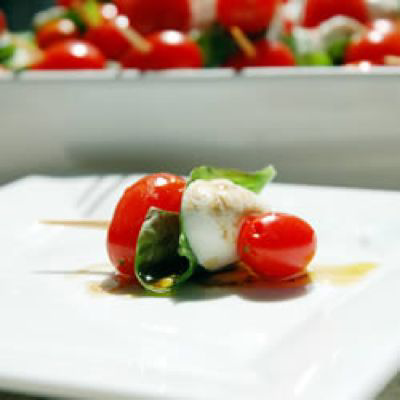
\includegraphics[width=0.9\linewidth]{/home/tim/Documents/projects/recipes/img/11D62489-861D-4C08-9951-A351CD643F10.jpg}\\
\end{minipage}\vspace{3mm}
\textbf{Directions}:
\vspace{-3mm}\begin{enumerate}\setlength\itemsep{-1mm}
\item Using a toothpick, spear a half of a tomato, a piece of basil, a mozzarella ball, and another half of a tomato. Repeat with remaining ingredients. Place on a serving dish and sprinkle with salt and pepper. Mix the vinegar and oil together in a small bowl to serve as a dipping sauce.
\end{enumerate}
\vspace{2mm}{\Large\textbf{Grilled Pizza With Strawberries and Chocolate}} \label{grilled-pizza-with-strawberries-and-chocolate}\hfill\textit{}\\
\begin{minipage}[t]{0.8\linewidth}
\textbf{Ingredients}:\vspace{-3mm}
\begin{multicols}{2}
\begin{itemize}\setlength\itemsep{-1mm}
\item 4 oz store - bought or homemade pizza dough, rolled thin
\item 1 Pint strawberry, sliced thinly
\item 1 1/2 tsp butter
\item 1/4 Cup chocolate chips
\item Canola oil spray
\item 1 cartoon of ice cream , for serving (optional)
\end{itemize}
\end{multicols}
\end{minipage}
\begin{minipage}[t]{0.2\linewidth}
\centering \strut\vspace*{-\baselineskip}\newline
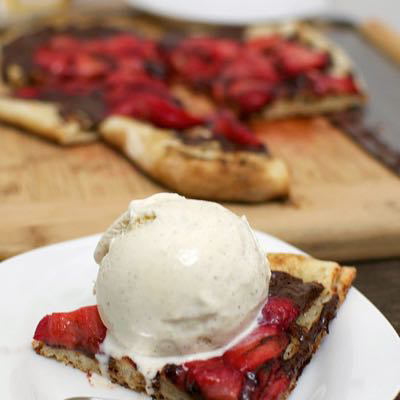
\includegraphics[width=0.9\linewidth]{/home/tim/Documents/projects/recipes/img/E8BDEA33-2F28-4313-A7AD-18CCDAD1F51B.jpg}\\
\end{minipage}\vspace{3mm}
\textbf{Directions}:
\vspace{-3mm}\begin{enumerate}\setlength\itemsep{-1mm}
\item Heat a charcoal or gas grill to high.
\item In a small saute pan, melt butter and gently saute the strawberries for 1 to 2 minutes.
\item Once the grill is hot, spray with canola oil spray to ensure the pizza doesn't stick. Add pizza dough, close the lid, and let the pizza cook for about 3-5 minutes depending on the thickness. Flip the pizza dough and cook for another 2-4 minutes.
\item Once the pizza begins to brown and grill marks appear, place the chocolate chips on top. Let melt for about 30 seconds, and spread the chocolate around with a small utensil. Top with strawberries and grill for another 30 seconds.
\item Remove the pizza from the grill, let cool slightly, and top with ice cream or whipping cream if desired.
\end{enumerate}
\vspace{2mm}{\Large\textbf{Pizza Dough}} \label{pizza-dough}\hfill\textit{}\\
\begin{minipage}[t]{0.8\linewidth}
\textbf{Ingredients}:\vspace{-3mm}
\begin{multicols}{2}
\begin{itemize}\setlength\itemsep{-1mm}
\item 1 Pack Active Dry Yeast
\item 1 Cup Warm Water
\item 1/2 tsp Salt
\item 1 tsp Sugar
\item 2 tsp Olive Oil
\item 3 Cups Flour
\end{itemize}
\end{multicols}
\end{minipage}
\begin{minipage}[t]{0.2\linewidth}
\centering \strut\vspace*{-\baselineskip}\newline
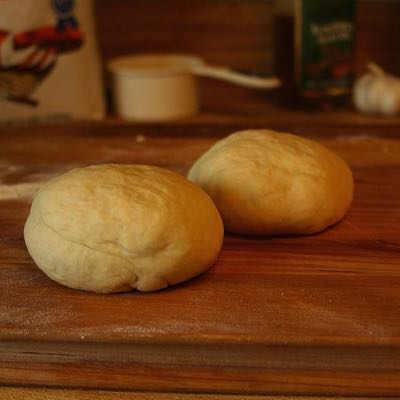
\includegraphics[width=0.9\linewidth]{/home/tim/Documents/projects/recipes/img/A8B5D904-A163-40ED-A6AF-9CA1CFB88DE0.jpg}\\
\end{minipage}\vspace{3mm}
\textbf{Directions}:
\vspace{-3mm}\begin{enumerate}\setlength\itemsep{-1mm}
\item Dissolve yeast in warm water(less than 100 degrees) in a large bowl.
\item Add salt, oil and 3 cups flour. Stir well.
\item Add flour until bowl is clean. 
\item Knead for 2 minutes or more.
\item Cover with a damp cloth or oiled plastic wrap and let rise for 1 hour.
\item Brush 14 inch pan with oil and bake at 450 degrees for 15 - 20 minutes. Tip: bake for five minutes, take out and put topping on, then bake for 15 minutes.
\end{enumerate}
\vspace{2mm}{\Large\textbf{Chicken Cordon Bleu}} \label{chicken-cordon-bleu}\hfill\textit{}\\
\begin{minipage}[t]{0.8\linewidth}
\textbf{Ingredients}:\vspace{-3mm}
\begin{multicols}{2}
\begin{itemize}\setlength\itemsep{-1mm}
\item 6 boneless skinless chicken breasts
\item 6 Slices (thin) lorraine swiss cheese
\item 6 (thin) slices maple ham
\item 3 Tbsp All-purpose flour
\item 1 tsp Paprika
\item 6 Tbsp Butter
\item 1/2 Cup Dry white wine
\item 1 tsp Chiken boullion (1 cube)
\item 1 Tbsp Cornstarch
\item 1 Cup Heavy whipping cream
\end{itemize}
\end{multicols}
\end{minipage}
\begin{minipage}[t]{0.2\linewidth}
\centering \strut\vspace*{-\baselineskip}\newline
\includegraphics[width=0.9\linewidth]{/home/tim/Documents/projects/recipes/img/}\\
\end{minipage}\vspace{3mm}
\textbf{Directions}:
\vspace{-3mm}\begin{enumerate}\setlength\itemsep{-1mm}
\item 1-Pound chicken breasts if too thick. Place cheese and ham on each breast. Fold chicken over filling and secure with toothpicks. Mix the flour and paprika in a small bowl and coat the chicken pieces.

2-heat the butter in a large skillet over medium high heat and cook the chicken until browned on all sides. Add the wine and bouillon. Reduce heat to low, cover and simmer for 30 minutes until chicken is no longer pink.

3-remove the toothpicks and transfer the breasts to a warm platter. Blend cornstarch with cream in a small bowl and whisk slowly into skillet. Cook, stirring until thickened, and pour over chicken. Serve warm. 
\end{enumerate}
\vspace{2mm}{\Large\textbf{Chocolate Brownies}} \label{chocolate-brownies}\hfill\textit{mom}\\
\begin{minipage}[t]{0.8\linewidth}
\textbf{Ingredients}:\vspace{-3mm}
\begin{multicols}{2}
\begin{itemize}\setlength\itemsep{-1mm}
\item 1/4 Cup Water
\item 2/3 Cup Vegetable oil
\item 2 Eggs
\item 1 Bag of Betty Crocker Fudge Brownie Mix
\end{itemize}
\end{multicols}
\end{minipage}
\begin{minipage}[t]{0.2\linewidth}
\centering \strut\vspace*{-\baselineskip}\newline
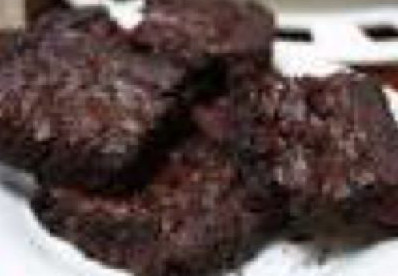
\includegraphics[width=0.9\linewidth]{/home/tim/Documents/projects/recipes/img/2C9BA575-680B-4B61-A6FE-35815E015DB6.jpg}\\
\end{minipage}\vspace{3mm}
\textbf{Directions}:
\vspace{-3mm}\begin{enumerate}\setlength\itemsep{-1mm}
\item 13"x9" - 350 - 24 to 26 minutes
9"x9" - 350 - 38 to 40 minutes
8"x8" - 325 - 52 to 54 minutes
\item Heat oven as directed above. Grease or use cooking spray.
\item Stir brownie mix, water, oil and eggs, in medium bowl until well blended. Spread in pan.
\item Bake as directed above, or until toothpick inserted 2 inches from side of pan comes out almost clean; cool. To cut warm brownies easily, cut with plastic knife using short sawing motions. Store tightly covered.
\end{enumerate}
\vspace{2mm}{\Large\textbf{Chocolate Mousse}} \label{chocolate-mousse}\hfill\textit{Cafe Elise}\\
\begin{minipage}[t]{0.8\linewidth}
\textbf{Ingredients}:\vspace{-3mm}
\begin{multicols}{2}
\begin{itemize}\setlength\itemsep{-1mm}
\item 1 1/2 lb Semisweet Chocolate
\item 3/4 lb Butter
\item 8 Yolks
\item 16 Whites
\item 3 Tbsp Sugar
\end{itemize}
\end{multicols}
\end{minipage}
\begin{minipage}[t]{0.2\linewidth}
\centering \strut\vspace*{-\baselineskip}\newline
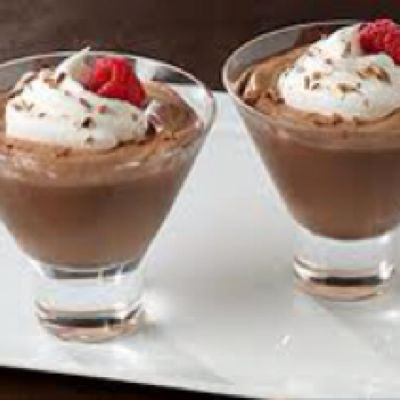
\includegraphics[width=0.9\linewidth]{/home/tim/Documents/projects/recipes/img/CC62DD46-9DF3-41E6-A455-99D21A28B627.jpg}\\
\end{minipage}\vspace{3mm}
\textbf{Directions}:
\vspace{-3mm}\begin{enumerate}\setlength\itemsep{-1mm}
\item Melt chocolate and butter over hot water. Whip in yolks.
\item Beat whites with sugar. (Firm, not stiff)
\item Fold together. Makes 30 portions. (4 ounces)
\end{enumerate}
\vspace{2mm}{\Large\textbf{Mint Meringues Recipe}} \label{mint-meringues-recipe}\hfill\textit{}\\
\begin{minipage}[t]{0.8\linewidth}
\textbf{Ingredients}:\vspace{-3mm}
\begin{multicols}{2}
\begin{itemize}\setlength\itemsep{-1mm}
\item 2 egg whites
\item 1/8 tsp salt
\item 1/8 tsp cream of tartar
\item 1/8 tsp peppermint extract
\item 6 drops green food coloring, optional
\item 1/2 Cup sugar
\item 1/3 Cup miniature semisweet chocolate chips
\end{itemize}
\end{multicols}
\end{minipage}
\begin{minipage}[t]{0.2\linewidth}
\centering \strut\vspace*{-\baselineskip}\newline
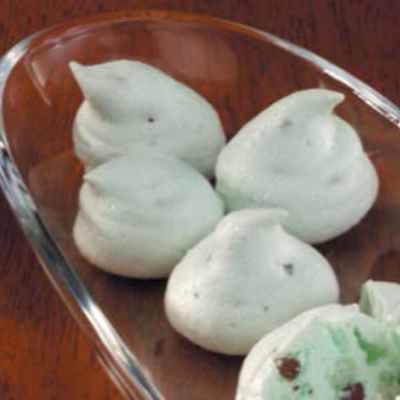
\includegraphics[width=0.9\linewidth]{/home/tim/Documents/projects/recipes/img/2F3BD676-F090-43F5-A86A-CA51F2F6D1A4.jpg}\\
\end{minipage}\vspace{3mm}
\textbf{Directions}:
\vspace{-3mm}\begin{enumerate}\setlength\itemsep{-1mm}
\item In a small bowl, beat the egg whites, salt, cream of tartar, extract and food coloring if desired on medium speed until soft peaks form. Gradually add sugar, 1 tablespoon at a time, beating on high until stiff glossy peaks form and sugar is dissolved, about 6 minutes. Gently fold in chocolate chips.
\item Drop by rounded teaspoonfuls 2 in. apart onto parchment paper-lined baking sheets. Bake at 250 for 40-45 minutes or until firm to the touch. Turn oven off; leave meringues in oven for 1-1/2 hours. Remove to wire racks. Store in an airtight container. Yield: 32 cookies.
\end{enumerate}
\vspace{2mm}{\Large\textbf{The Best Steak Marinade}} \label{the-best-steak-marinade}\hfill\textit{allrecipes.com}\\
\begin{minipage}[t]{0.8\linewidth}
\textbf{Ingredients}:\vspace{-3mm}
\begin{multicols}{2}
\begin{itemize}\setlength\itemsep{-1mm}
\item 1/4 Cup olive oil
\item 1/4 Cup balsamic vinegar
\item 1/4 Cup Worcestershire sauce
\item 1/4 Cup soy sauce
\item 2 tsp Dijon mustard
\item 2 tsp minced garlic
\item salt and pepper to taste
\end{itemize}
\end{multicols}
\end{minipage}
\begin{minipage}[t]{0.2\linewidth}
\centering \strut\vspace*{-\baselineskip}\newline
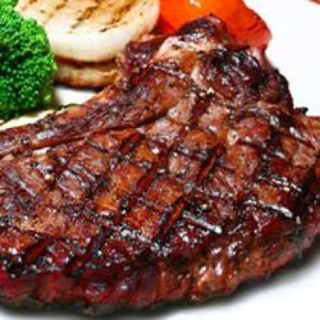
\includegraphics[width=0.9\linewidth]{/home/tim/Documents/projects/recipes/img/4F7D32C0-C8F8-4DBA-947B-5A67096B5D1D.jpg}\\
\end{minipage}\vspace{3mm}
\textbf{Directions}:
\vspace{-3mm}\begin{enumerate}\setlength\itemsep{-1mm}
\item Mix olive oil, balsamic vinegar, Worcestershire sauce, soy sauce, Dijon mustard, and garlic in a small bowl. Season with salt and pepper.
\end{enumerate}
\vspace{2mm}{\Large\textbf{Crispy Crunchy Chocolate Chip Cookies}} \label{crispy-crunchy-chocolate-chip-cookies}\hfill\textit{}\\
\begin{minipage}[t]{0.8\linewidth}
\textbf{Ingredients}:\vspace{-3mm}
\begin{multicols}{2}
\begin{itemize}\setlength\itemsep{-1mm}
\item 1 Cup Ghirardelli Semi - Sweet Chocolate Chips
\item 1 1/3 Cups all purpose flour
\item 1/2 tsp baking soda
\item 1/2 tsp salt
\item 10 Tbsp unsalted butter, melted and cooled (1 1/4 sticks)
\item 1/3 Cup lightly packed light brown sugar
\item 1/4 Cup granulated sugar
\item 2 Tbsp light corn syrup
\item 2 Tbsp milk
\item 1 tsp vanilla extract
\item 3/4 to 1 cup chopped pecans or walnuts
\end{itemize}
\end{multicols}
\end{minipage}
\begin{minipage}[t]{0.2\linewidth}
\centering \strut\vspace*{-\baselineskip}\newline
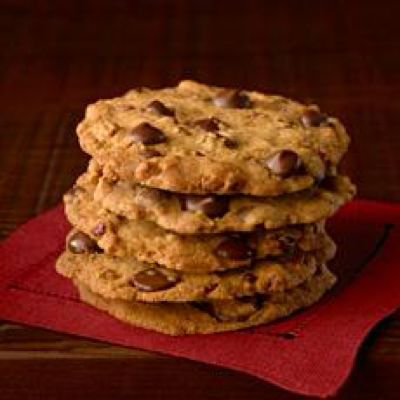
\includegraphics[width=0.9\linewidth]{/home/tim/Documents/projects/recipes/img/733A7250-2033-41F5-BE08-06DD7EF25077.jpg}\\
\end{minipage}\vspace{3mm}
\textbf{Directions}:
\vspace{-3mm}\begin{enumerate}\setlength\itemsep{-1mm}
\item Directions
\item Position racks in the upper and lower thirds of the oven. Preheat the oven to 325F. Line two large baking sheets with foil, dull side up. Mix the flour, baking soda, and salt together thoroughly. Set aside. In a large bowl, combine the butter, both sugars, corn syrup, milk, and vanilla. Mix until smooth. Stir in the flour mixture. Stir in the nuts and chocolate chips. The dough will be very soft.
\item Divide the dough in half. Divide one half of the dough into 10 equal pieces (each a scant 1/4 cup). Place 5 pieces of dough least 3 inches apart on each lined baking sheet. Use your fingers covered with a piece of plastic wrap to flatten each scoop until it is 3 inches in diameter. (Cookies will spread even more as they bake).
\item Bake the two sheets for 8 minutes. Rotate the sheets from the top rack to the bottom and from front to back. Bake for 7-10 more minutes, watching closely, until the cookies are evenly dark golden brown all over. (Pale cookies will not be crispy). Let cool on pan for 5 minutes. Slide the foil with cookies onto racks. When the baking sheets are cool, repeat with the remaining dough. Cool cookies completely before stacking or storing. Cookies keep, in an airtight container for at least 5 days.
\end{enumerate}
\vspace{2mm}{\Large\textbf{Grandma Dunn's Rib Sauce}} \label{grandma-dunn's-rib-sauce}\hfill\textit{Grandma Dunn}\\
\begin{minipage}[t]{0.8\linewidth}
\textbf{Ingredients}:\vspace{-3mm}
\begin{multicols}{2}
\begin{itemize}\setlength\itemsep{-1mm}
\item 1 Cup OJ
\item 1 Lemon
\item 1 Cup Brown Sugar
\item 3/4 Cup Pancake syrup
\item Celery
\item 1 Onion
\item 1 Tbsp Worcestershire sauce
\item 3 Tbsp Vinegar
\item 1 Tbsp dry mustard
\item Parsley
\item 1 Cup ketchup
\end{itemize}
\end{multicols}
\end{minipage}
\begin{minipage}[t]{0.2\linewidth}
\centering \strut\vspace*{-\baselineskip}\newline
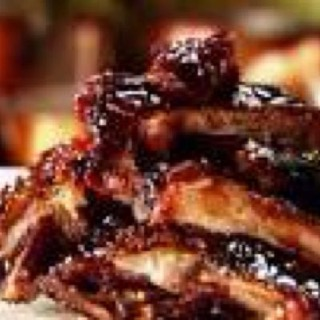
\includegraphics[width=0.9\linewidth]{/home/tim/Documents/projects/recipes/img/8046BA7D-6BD0-4D87-A0B7-3EC284E1A15A.jpg}\\
\end{minipage}\vspace{3mm}
\textbf{Directions}:
\vspace{-3mm}\begin{enumerate}\setlength\itemsep{-1mm}
\item Pour sauce on ribs or chicken. Cook at 325 for 2 hours. Turn off oven and let sit.
\end{enumerate}
\vspace{2mm}{\Large\textbf{Blueberry Kuchen Recipe}} \label{blueberry-kuchen-recipe}\hfill\textit{}\\
\begin{minipage}[t]{0.8\linewidth}
\textbf{Ingredients}:\vspace{-3mm}
\begin{multicols}{2}
\begin{itemize}\setlength\itemsep{-1mm}
\item 1 Cup Flour
\item 1/8 tsp salt
\item 2 Tbsp Sugar
\item 1/2 Cup butter, slightly softened and cut into small pieces (8 tablespoons)
\item 1 Tbsp white vinegar
\item 5 Cups fresh blueberries (725 grams)
\item 1/2 Cup sugar
\item 1/8 tsp cinnamon
\item 2 Tbsp Flour
\end{itemize}
\end{multicols}
\end{minipage}
\begin{minipage}[t]{0.2\linewidth}
\centering \strut\vspace*{-\baselineskip}\newline
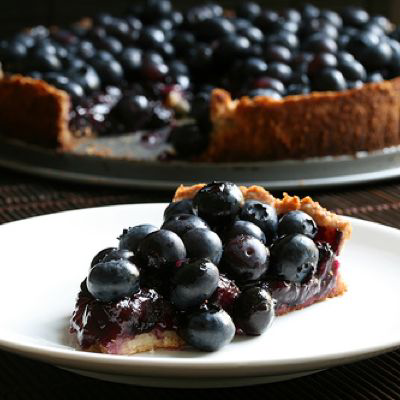
\includegraphics[width=0.9\linewidth]{/home/tim/Documents/projects/recipes/img/F3625974-C436-4C8A-B7FB-4B55F0391AEF.jpg}\\
\end{minipage}\vspace{3mm}
\textbf{Directions}:
\vspace{-3mm}\begin{enumerate}\setlength\itemsep{-1mm}
\item Preheat oven to 350 F. In medium bowl, mix 1 cup flour, salt and 2 tablespoons sugar. Cut in butter until it resembles coarse crumbs. Sprinkle with vinegar and shape into dough. With lightly floured fingers, press dough into 9-inch springform pan about 1/4 inch thickness on bottom, less thick and 1 inch high around the sides.
\item Mix 3 cups blueberries, 2 tablespoon flour, 1/2 cup sugar and cinnamon. Pour and spread the blueberries onto the crust and bake on the middle rack for 20 minutes or until crust is golden brown and filling bubbles. Remove from oven and place on cooling rack. Sprinkle with remaining 2 cups blueberries. Cool for at least 30 minutes. Run a pairing knife around the crust edge to separate from the pan before opening springform.  Serve with a scoop of vanilla ice cream.
\end{enumerate}
\vspace{2mm}{\Large\textbf{Apple Cobbler}} \label{apple-cobbler}\hfill\textit{Recipe Book Selections}\\
\begin{minipage}[t]{0.8\linewidth}
\textbf{Ingredients}:\vspace{-3mm}
\begin{multicols}{2}
\begin{itemize}\setlength\itemsep{-1mm}
\item 6 Large Apples (Peeled, cored and sliced)
\item 3 Tbsp Cinnamon (to taste)
\item 2 Tbsp Lime or lemon juice
\item 2 Tbsp Sugar (sub splenda)
\item 1/4 Cup Apple Cider
\item 2 Cups Instant Oatmeal
\item 1/4 Cup Butter (Melted)
\item 1/4 Cup Brown Sugar
\item 2 Tbsp Cinnamon
\end{itemize}
\end{multicols}
\end{minipage}
\begin{minipage}[t]{0.2\linewidth}
\centering \strut\vspace*{-\baselineskip}\newline
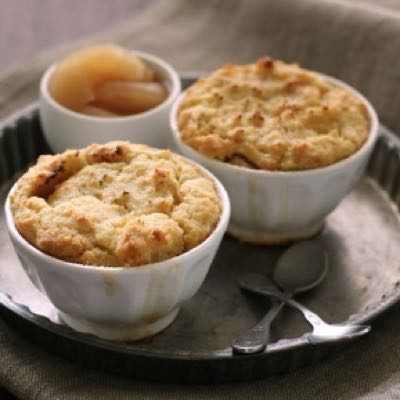
\includegraphics[width=0.9\linewidth]{/home/tim/Documents/projects/recipes/img/55A3A7DC-5599-4D56-AA7B-5AD622436662.jpg}\\
\end{minipage}\vspace{3mm}
\textbf{Directions}:
\vspace{-3mm}\begin{enumerate}\setlength\itemsep{-1mm}
\item Mix filling ingredients (apples, 3 tbsp cinnamon,lime, sugar and cider) together and chill for at least 1 hour.
\item Toss filling with apple cider.
\item Pour into greased oven safe pan.
\item Mix topping ingredients together thoroughly and spread on top.
\item Bake at 350 degrees for 45-60 minutes or until apples are tender and bubbly.
\end{enumerate}
\vspace{2mm}{\Large\textbf{Bran Muffins}} \label{bran-muffins}\hfill\textit{}\\
\begin{minipage}[t]{0.8\linewidth}
\textbf{Ingredients}:\vspace{-3mm}
\begin{multicols}{2}
\begin{itemize}\setlength\itemsep{-1mm}
\item 3 1/2 Cups Bran
\item 1/2 Large box Raisins
\item 1 Cup Boiling water
\item 1/2 Cup Honey
\item 1/2 Cup Corn oil
\item 3/4 Cup Molasses
\item 2 Eggs
\item 2 Cups Buttermilk
\item 1 1/2 Cups Whole wheat flour
\item 2 1/2 tsp Baking soda
\item 1/2 tsp Salt
\end{itemize}
\end{multicols}
\end{minipage}
\begin{minipage}[t]{0.2\linewidth}
\centering \strut\vspace*{-\baselineskip}\newline
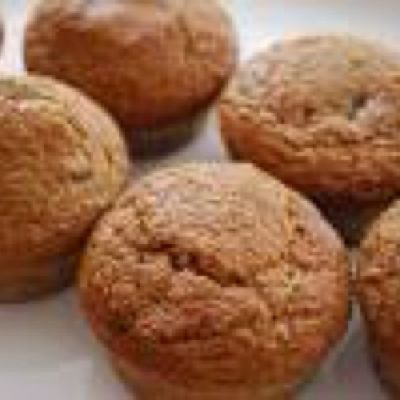
\includegraphics[width=0.9\linewidth]{/home/tim/Documents/projects/recipes/img/DA1F4361-D9DD-4F32-A670-078982804C92.jpg}\\
\end{minipage}\vspace{3mm}
\textbf{Directions}:
\vspace{-3mm}\begin{enumerate}\setlength\itemsep{-1mm}
\item Preheat oven to 400
\item 2 cups of bran and raisins and add boiling water
\item Measure oil first, then mix with honey, molasses, eggs and buttermilk in separate bowl
\item Add flour, rest of bran, soda and salt to above
\item Stir in bran raisin mixture
\item Spoon into muffin cups about 2/3 full. (They rise)
\item Cook for 20 minutes
\item Keep leftover mixture in fridge, since it keeps for several weeks. Can make instant muffins with microwave.
\end{enumerate}
\vspace{2mm}{\Large\textbf{Zucchini Bread}} \label{zucchini-bread}\hfill\textit{allrecipes.com}\\
\begin{minipage}[t]{0.8\linewidth}
\textbf{Ingredients}:\vspace{-3mm}
\begin{multicols}{2}
\begin{itemize}\setlength\itemsep{-1mm}
\item 3 Cups all - purpose flour
\item 1 tsp salt
\item 1 tsp baking soda
\item 1 tsp baking powder
\item 3 tsp ground cinnamon
\item 3 eggs
\item 1 Cup vegetable oil
\item 2 1/4 Cups white sugar
\item 3 tsp vanilla extract
\item 2 Cups grated zucchini
\item 1 Cup chopped walnuts
\end{itemize}
\end{multicols}
\end{minipage}
\begin{minipage}[t]{0.2\linewidth}
\centering \strut\vspace*{-\baselineskip}\newline
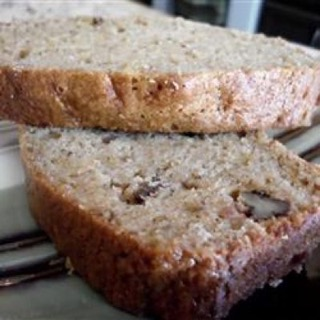
\includegraphics[width=0.9\linewidth]{/home/tim/Documents/projects/recipes/img/3671A514-1C82-49BB-B842-F8A855CF46B6.jpg}\\
\end{minipage}\vspace{3mm}
\textbf{Directions}:
\vspace{-3mm}\begin{enumerate}\setlength\itemsep{-1mm}
\item Grease and flour two 8 x 4 inch pans. Preheat oven to 325 degrees F (165 degrees C).
\item Sift flour, salt, baking powder, soda, and cinnamon together in a bowl.
\item Beat eggs, oil, vanilla, and sugar together in a large bowl. Add sifted ingredients to the creamed mixture, and beat well. Stir in zucchini and nuts until well combined. Pour batter into prepared pans.
\item Bake for 40 to 60 minutes, or until tester inserted in the center comes out clean. Cool in pan on rack for 20 minutes. Remove bread from pan, and completely cool.
\end{enumerate}
\vspace{2mm}{\Large\textbf{Russian Tea Cakes}} \label{russian-tea-cakes}\hfill\textit{www.bettycrocker.com}\\
\begin{minipage}[t]{0.8\linewidth}
\textbf{Ingredients}:\vspace{-3mm}
\begin{multicols}{2}
\begin{itemize}\setlength\itemsep{-1mm}
\item 1 cup butter or margarine, softened
\item 1/2 cup powdered sugar
\item 1 teaspoon vanilla
\item 2 1/4 cups Gold Medal all - purpose flour
\item 3/4 cup finely chopped nuts
\item 1/4 teaspoon salt
\item Powdered sugar
\end{itemize}
\end{multicols}
\end{minipage}
\begin{minipage}[t]{0.2\linewidth}
\centering \strut\vspace*{-\baselineskip}\newline
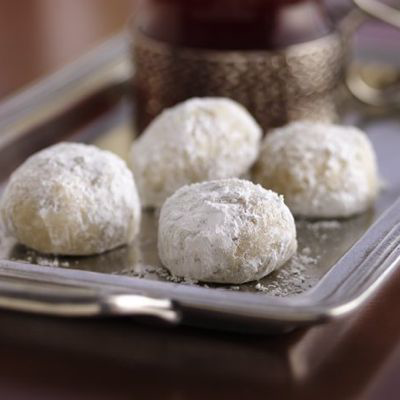
\includegraphics[width=0.9\linewidth]{/home/tim/Documents/projects/recipes/img/05B2E5B1-94ED-4006-BB76-8CE6F0BE54F0.jpg}\\
\end{minipage}\vspace{3mm}
\textbf{Directions}:
\vspace{-3mm}\begin{enumerate}\setlength\itemsep{-1mm}
\item Heat oven to 375 F.
\item Mix butter, 1/2 cup powdered sugar and the vanilla in large bowl. Stir in flour, nuts and salt until dough holds together.
\item Shape dough into 1-inch balls. Place about 1 inch apart on ungreased cookie sheet.
\item Bake 10 to 12 minutes or until set but not brown. Remove from cookie sheet. Cool slightly on wire rack.
\item Roll warm cookies in powdered sugar; cool on wire rack. Roll in powdered sugar again.
\end{enumerate}
\vspace{2mm}{\Large\textbf{Christmas Crackle}} \label{christmas-crackle}\hfill\textit{Aimee Rinere}\\
\begin{minipage}[t]{0.8\linewidth}
\textbf{Ingredients}:\vspace{-3mm}
\begin{multicols}{2}
\begin{itemize}\setlength\itemsep{-1mm}
\item 14 Cups Microwave popcorn, popped (about 2 bags)
\item 3 Cups Rice Krispies cereal
\item 2 Cups Mixed salted nuts
\item 1 lb white chocolate
\item 3 Tbsp Peanut butter
\end{itemize}
\end{multicols}
\end{minipage}
\begin{minipage}[t]{0.2\linewidth}
\centering \strut\vspace*{-\baselineskip}\newline
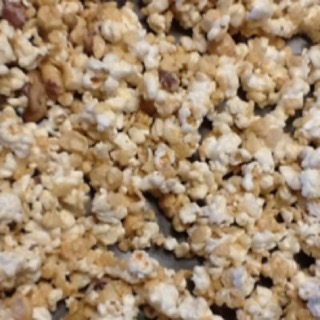
\includegraphics[width=0.9\linewidth]{/home/tim/Documents/projects/recipes/img/F6310104-FB28-461F-A8A3-24990DCB4E48.jpg}\\
\end{minipage}\vspace{3mm}
\textbf{Directions}:
\vspace{-3mm}\begin{enumerate}\setlength\itemsep{-1mm}
\item Mix popcorn, Rice Krispies and nuts in a large bowl.
\item In the microwave melt:

white chocolate and peanut butter. Start with 1 minute then stir and repeat until melted and smooth. Pour over the popcorn and mix well. Spread onto wax paper and let set for about 2 hours. Break apart into pieces.
\end{enumerate}
\vspace{2mm}{\Large\textbf{Chicken Devan}} \label{chicken-devan}\hfill\textit{Mom}\\
\begin{minipage}[t]{0.8\linewidth}
\textbf{Ingredients}:\vspace{-3mm}
\begin{multicols}{2}
\begin{itemize}\setlength\itemsep{-1mm}
\item 2 Pkg. Broccoli cuts (i like to used chopped)
\item 3 Whole Chicken breasts (cooked, boned and cut in pieces)
\item 2 Cans condensed cream of chicken soup (i use Campbells healthy choice)
\item 1 Cup mayonnaise (light is fine)
\item 1 tsp lemon juice
\item 1/2 tsp Curry powder
\item 1 Cup shredded Cheddar cheese
\end{itemize}
\end{multicols}
\end{minipage}
\begin{minipage}[t]{0.2\linewidth}
\centering \strut\vspace*{-\baselineskip}\newline
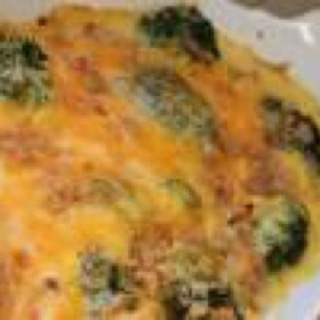
\includegraphics[width=0.9\linewidth]{/home/tim/Documents/projects/recipes/img/BEFEED18-A837-4235-853D-6933B6FB94FE.jpg}\\
\end{minipage}\vspace{3mm}
\textbf{Directions}:
\vspace{-3mm}\begin{enumerate}\setlength\itemsep{-1mm}
\item Place broccoli in 9x13 pan season with salt and pepper. Place chicken on top, make a sauce of soup, mayo, lemon juice and curry. Pour over above, sprinkle with cheese.
\item Bake 30 mins at 350
\end{enumerate}
\vspace{2mm}{\Large\textbf{Vanilla Crepes}} \label{vanilla-crepes}\hfill\textit{allrecipes.com}\\
\begin{minipage}[t]{0.8\linewidth}
\textbf{Ingredients}:\vspace{-3mm}
\begin{multicols}{2}
\begin{itemize}\setlength\itemsep{-1mm}
\item 1 1/2 Cups milk
\item 3 egg yolks
\item 2 Tbsp vanilla extract
\item 1 1/2 Cups all - purpose flour
\item 2 Tbsp sugar
\item 1/2 tsp salt
\item 5 Tbsp melted butter
\end{itemize}
\end{multicols}
\end{minipage}
\begin{minipage}[t]{0.2\linewidth}
\centering \strut\vspace*{-\baselineskip}\newline
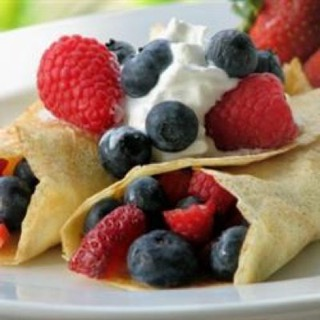
\includegraphics[width=0.9\linewidth]{/home/tim/Documents/projects/recipes/img/0B83F7B6-936B-4567-8F9C-43D0D9D10A6A.jpg}\\
\end{minipage}\vspace{3mm}
\textbf{Directions}:
\vspace{-3mm}\begin{enumerate}\setlength\itemsep{-1mm}
\item In a large bowl, mix together the milk, egg yolks and vanilla. Stir in the flour, sugar, salt and melted butter until well blended.
\item Heat a crepe pan over medium heat until hot. Coat with vegetable oil or cooking spray. Pour about 1/4 cup of batter into the pan and tip to spread the batter to the edges. When bubbles form on the top and the edges are dry, flip over and cook until lightly browned on the other side and edges are golden. Repeat with remaining batter.
\item Fill crepes with your favorite fruit, cream, caramel or even ice cream or cheese to serve.
\end{enumerate}
\vspace{2mm}{\Large\textbf{Chocolate Cherry Milkshake}} \label{chocolate-cherry-milkshake}\hfill\textit{}\\
\begin{minipage}[t]{0.8\linewidth}
\textbf{Ingredients}:\vspace{-3mm}
\begin{multicols}{2}
\begin{itemize}\setlength\itemsep{-1mm}
\item 4 scoops vanilla ice cream or frozen yogurt (about 2 cups)
\item 3/4 Cup cold milk
\item 1/4 Cup HERSHEY'S Syrup
\item 8 maraschino cherries, stems removed
\item Whipped topping & additional cherry (optional)
\end{itemize}
\end{multicols}
\end{minipage}
\begin{minipage}[t]{0.2\linewidth}
\centering \strut\vspace*{-\baselineskip}\newline

\includegraphics[width=0.9\linewidth]{/home/tim/Documents/projects/recipes/img/0A51010C-1D44-4BF3-924D-DAED421C55DD.jpg}\\
\end{minipage}\vspace{3mm}
\textbf{Directions}:
\vspace{-3mm}\begin{enumerate}\setlength\itemsep{-1mm}
\item Place ice cream, milk, syrup and cherries in blender container. Cover; blend until smooth.
\item Garnish with whipped topping and cherry, if desired. Two 10-oz. servings.
\end{enumerate}
\vspace{2mm}{\Large\textbf{Broccoli Chicken Casserole}} \label{broccoli-chicken-casserole}\hfill\textit{Nancy Feth}\\
\begin{minipage}[t]{0.8\linewidth}
\textbf{Ingredients}:\vspace{-3mm}
\begin{multicols}{2}
\begin{itemize}\setlength\itemsep{-1mm}
\item 2 (10 oz.) packages Broccoli cuts
\item 3 Whole Chicken breasts (cooked, boned and cut in pieces)
\item 2 Cans condensed cream of chicken soup
\item 1 Cup mayonnaise
\item 1 tsp lemon juice
\item 1/2 tsp Curry powder
\item 1 Cup shredded sharp Cheddar cheese
\end{itemize}
\end{multicols}
\end{minipage}
\begin{minipage}[t]{0.2\linewidth}
\centering \strut\vspace*{-\baselineskip}\newline
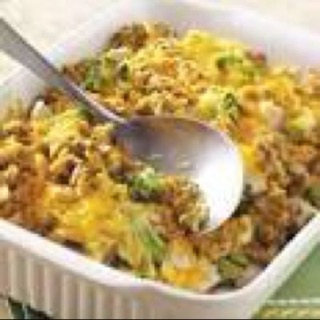
\includegraphics[width=0.9\linewidth]{/home/tim/Documents/projects/recipes/img/B22FE9D1-F626-4C5B-B0BD-B4F423DB41FA.jpg}\\
\end{minipage}\vspace{3mm}
\textbf{Directions}:
\vspace{-3mm}\begin{enumerate}\setlength\itemsep{-1mm}
\item Place uncooked broccoli in 9x13 baking dish. Season with salt and pepper.
\item Place cut-up chicken pieces on top. Make a sauce with soup, mayonnaise, lemon juice and curry powder. Pour over chicken. Sprinkle with cheese.
\item Bake for 30 minutes at 350F
\item If made 1 day in advance, refrigerate and bake slightly longer
\end{enumerate}
\vspace{2mm}{\Large\textbf{Almond Macaroons}} \label{almond-macaroons}\hfill\textit{}\\
\begin{minipage}[t]{0.8\linewidth}
\textbf{Ingredients}:\vspace{-3mm}
\begin{multicols}{2}
\begin{itemize}\setlength\itemsep{-1mm}
\item 10 oz blanched whole almonds (about 2 full cups)
\item 2 3/4 Cups granulated sugar
\item 3 Large egg whites
\item 1/2 tsp pure almond extract
\item 6 oz good quality bittersweet chocolate, chopped (optional)
\end{itemize}
\end{multicols}
\end{minipage}
\begin{minipage}[t]{0.2\linewidth}
\centering \strut\vspace*{-\baselineskip}\newline
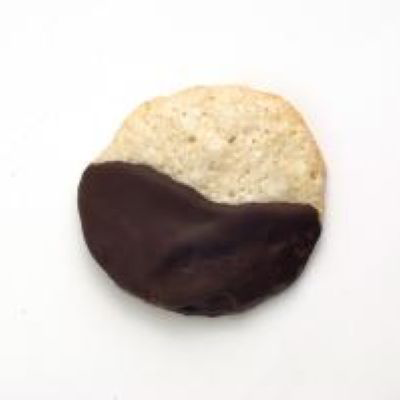
\includegraphics[width=0.9\linewidth]{/home/tim/Documents/projects/recipes/img/DD993399-6C6B-4C84-ADE9-9D35E6F5E3F3.jpg}\\
\end{minipage}\vspace{3mm}
\textbf{Directions}:
\vspace{-3mm}\begin{enumerate}\setlength\itemsep{-1mm}
\item Preheat oven to 350 degrees. Line one or two cookie sheets with parchment paper.
\item Combine the almonds and 1/4 cup of the sugar in a food processor and process until the almonds are finely ground. Add the egg whites and almond extract and process until blended.
\item Add the remaining 1 cup of sugar and process until thoroughly combined, about 15 seconds, or until the dough is a thick, sticky paste.
\item Drop the dough by level tablespoonfuls, arranging about 2 inches apart on the prepared sheet(s). Using a pastry brush lightly moistened with water, brush the tops and sides of the macaroons, gently pressing down on them to form smooth rounds about 1/2 inch thick and 1 3/4 inches in diameter.
\item Bake for about 15 minutes or until the macaroons are pale golden. They should feel crisp on the outside but still soft inside. (If using two cookie sheets, rotate them from top to bottom and front to back about halfway through baking.) Remove the sheets from the oven and slide the parchment onto racks. Cool for about 5 minutes, then use a thin metal spatula to remove the macaroons from the paper. Place on rack to cool.
\item For chocolate-dipped macaroons, melt the chocolate in a metal or glass bowl set over a pan of barely simmering water, stirring frequently, until fully melted. Alternatively, melt it in a microwave-safe bowl in microwave, using 20-to-30-second bursts at medium power, stirring well after each interval. Line baking sheet with wax paper. With a silicone pastry brush, brush the melted chocolate on half the cookie, both top side and bottom, in a semicircle. Let the excess drip off or gently scrape it off the bottom using the brush. Place the macaroons on the wax paper and let stand until the chocolate is completely set.
\item Store macaroons in an airtight container, layered between sheets of wax paper, for up to five days at room temperature. Macaroons without chocolate can be frozen for up to two months.
\end{enumerate}
\vspace{2mm}{\Large\textbf{Extreme Chocolate Cake}} \label{extreme-chocolate-cake}\hfill\textit{}\\
\begin{minipage}[t]{0.8\linewidth}
\textbf{Ingredients}:\vspace{-3mm}
\begin{multicols}{2}
\begin{itemize}\setlength\itemsep{-1mm}
\item 2 Cups white sugar
\item 1 3/4 Cups all - purpose flour
\item 3/4 Cup unsweetened cocoa powder
\item 1 1/2 tsp baking soda
\item 1 1/2 tsp baking powder
\item 1 tsp salt
\item 2 eggs
\item 1 Cup milk
\item 1/2 Cup vegetable oil
\item 2 tsp vanilla extract
\item 1 Cup boiling water
\item  
\item 3/4 Cup butter
\item 1 1/2 Cups unsweetened cocoa powder
\item 5 1/3 Cups confectioners' sugar
\item 2/3 Cup milk
\item 1 tsp vanilla extract
\end{itemize}
\end{multicols}
\end{minipage}
\begin{minipage}[t]{0.2\linewidth}
\centering \strut\vspace*{-\baselineskip}\newline
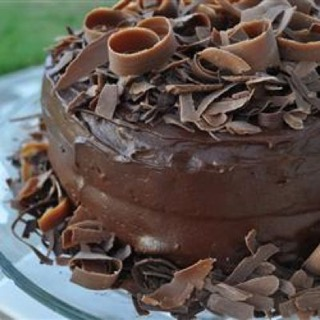
\includegraphics[width=0.9\linewidth]{/home/tim/Documents/projects/recipes/img/A52E86A7-64B0-4BB1-BA54-F0C460F9DAB1.jpg}\\
\end{minipage}\vspace{3mm}
\textbf{Directions}:
\vspace{-3mm}\begin{enumerate}\setlength\itemsep{-1mm}
\item Preheat oven to 350 degrees F (175 degrees C). Grease and flour two 9 inch cake pans.
\item Use the first set of ingredients to make the cake. In a medium bowl, stir together the sugar, flour, cocoa, baking soda, baking powder and salt. Add the eggs, milk, oil and vanilla, mix for 3 minutes with an electric mixer. Stir in the boiling water by hand. Pour evenly into the two prepared pans.
\item Bake for 30 to 35 minutes in the preheated oven, until a toothpick inserted comes out clean. Cool for 10 minutes before removing from pans to cool completely.
\item To make the frosting, use the second set of ingredients. Cream butter until light and fluffy. Stir in the cocoa and confectioners' sugar alternately with the milk and vanilla. Beat to a spreading consistency.
\item Split the layers of cooled cake horizontally, cover the top of each layer with frosting, then stack them onto a serving plate. Frost the outside of the cake.
\end{enumerate}
\vspace{2mm}{\Large\textbf{Cookies 'n Creme Brownies}} \label{cookies-'n-creme-brownies}\hfill\textit{}\\
\begin{minipage}[t]{0.8\linewidth}
\textbf{Ingredients}:\vspace{-3mm}
\begin{multicols}{2}
\begin{itemize}\setlength\itemsep{-1mm}
\item 1 
\item box Betty Crocker fudge brownie mix (1 lb 2.3 oz)
\item 1/4 
\item cup water
\item 2/3 
\item cup vegetable oil
\item 2 
\item eggs
\item 10 
\item creme - filled chocolate sandwich cookies, crushed (1 cup)
\item 1/2 
\item container Betty Crocker Rich & Creamy chocolate or vanilla frosting (2/3 cup) (16 - oz size)
\item 5 
\item creme - filled chocolate sandwich cookies, coarsely chopped (2/3 cup)
\end{itemize}
\end{multicols}
\end{minipage}
\begin{minipage}[t]{0.2\linewidth}
\centering \strut\vspace*{-\baselineskip}\newline
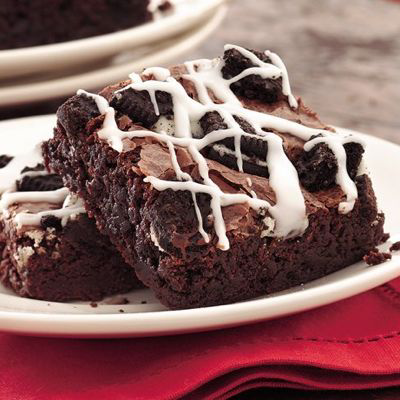
\includegraphics[width=0.9\linewidth]{/home/tim/Documents/projects/recipes/img/C97952C2-0F95-4E79-AAA2-59EB9E434D5F.jpg}\\
\end{minipage}\vspace{3mm}
\textbf{Directions}:
\vspace{-3mm}\begin{enumerate}\setlength\itemsep{-1mm}
\item Heat oven to 350F. Grease bottom only of rectangular pan, 13x9x2 inches, or spray with cooking spray.
\item Stir brownie mix, water, oil and eggs in medium bowl until well blended. Stir in 1 cup crushed cookies. Spread in pan.
\item Bake 24 to 26 minutes or until toothpick inserted 2 inches from side of pan comes out clean or almost clean. Cool completely, about 1 hour. In small microwavable bowl, microwave frosting uncovered on High about 10 to 15 seconds or until drizzling consistency. Drizzle frosting over brownies. Sprinkle with 2/3 cup chopped cookies. For 20 brownies, cut into 5 rows by 4 rows.
\end{enumerate}
\vspace{2mm}{\Large\textbf{Slow Cooker Meaty Italian Spaghetti Sauce}} \label{slow-cooker-meaty-italian-spaghetti-sauce}\hfill\textit{}\\
\begin{minipage}[t]{0.8\linewidth}
\textbf{Ingredients}:\vspace{-3mm}
\begin{multicols}{2}
\begin{itemize}\setlength\itemsep{-1mm}
\item 2 
\item lb bulk Italian pork sausage or ground beef
\item 2 
\item large onions, chopped (2 cups)
\item 2 
\item cups sliced fresh mushrooms (6 oz)
\item 3 
\item cloves garlic, finely chopped
\item 1 
\item can Muir Glen organic diced tomatoes, undrained (28 oz)
\item 2 
\item cans tomato sauce (15 oz each)
\item 1 
\item can tomato paste (6 oz)
\item 1 
\item tablespoon dried basil leaves
\item 1 
\item teaspoon dried oregano leaves
\item 1 
\item tablespoon sugar
\item 1/2 
\item teaspoon salt
\item 1/2 
\item teaspoon pepper
\item 1/2 
\item teaspoon crushed red pepper flakes
\end{itemize}
\end{multicols}
\end{minipage}
\begin{minipage}[t]{0.2\linewidth}
\centering \strut\vspace*{-\baselineskip}\newline
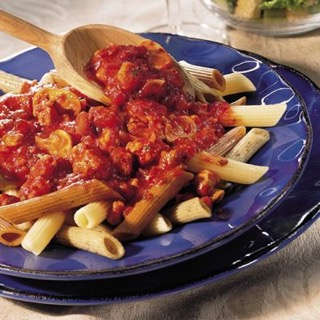
\includegraphics[width=0.9\linewidth]{/home/tim/Documents/projects/recipes/img/554650A2-957E-41C2-A677-E8F43CB4542E.jpg}\\
\end{minipage}\vspace{3mm}
\textbf{Directions}:
\vspace{-3mm}\begin{enumerate}\setlength\itemsep{-1mm}
\item Spray 5-quart slow cooker with cooking spray. In 12-inch skillet, cook sausage, onions, mushrooms and garlic over medium heat about 10 minutes, stirring occasionally, until sausage is no longer pink; drain.
\item Spoon sausage mixture into cooker. Stir in remaining ingredients.
\item Cover; cook on Low heat setting 8 to 9 hours.
\end{enumerate}
\vspace{2mm}{\Large\textbf{Dark Chocolate Brownies}} \label{dark-chocolate-brownies}\hfill\textit{Carolyn Benjamin}\\
\begin{minipage}[t]{0.8\linewidth}
\textbf{Ingredients}:\vspace{-3mm}
\begin{multicols}{2}
\begin{itemize}\setlength\itemsep{-1mm}
\item 1 Cup margarine
\item 1 Cup Cocoa powder (unsweetened)
\item 4 Eggs
\item 2 Cups Sugar
\item 1/4 tsp Salt
\item 1 tsp Vanilla
\item 1 Cup Flour
\item 1 Cup Chopped chocolate or chocolate chips
\end{itemize}
\end{multicols}
\end{minipage}
\begin{minipage}[t]{0.2\linewidth}
\centering \strut\vspace*{-\baselineskip}\newline
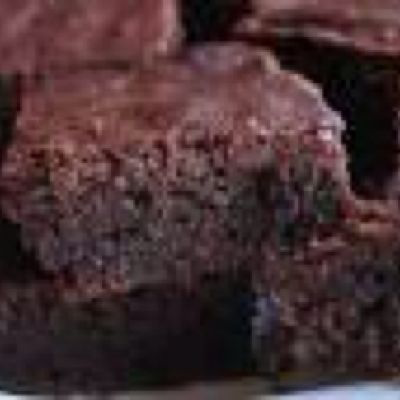
\includegraphics[width=0.9\linewidth]{/home/tim/Documents/projects/recipes/img/8C974ABB-FAF0-4069-ABC9-A068D28D8FCA.jpg}\\
\end{minipage}\vspace{3mm}
\textbf{Directions}:
\vspace{-3mm}\begin{enumerate}\setlength\itemsep{-1mm}
\item Melt margarine and stir cocoa-set aside. Beat eggs with sugar, salt and vanilla. Combine with margarine cocoa mixture. Add flour and chopped chocolate. Bake in greased 9x13" pan at 350 for 20 minutes and check. May need a few more minutes.
\item Mix by hand! No mixer
\end{enumerate}
\vspace{2mm}{\Large\textbf{Basic Crepes}} \label{basic-crepes}\hfill\textit{allrecipes.com}\\
\begin{minipage}[t]{0.8\linewidth}
\textbf{Ingredients}:\vspace{-3mm}
\begin{multicols}{2}
\begin{itemize}\setlength\itemsep{-1mm}
\item 1 Cup all - purpose flour
\item 2 eggs
\item 1/2 Cup milk
\item 1/2 Cup water
\item 1/4 tsp salt
\item 2 Tbsp butter, melted
\end{itemize}
\end{multicols}
\end{minipage}
\begin{minipage}[t]{0.2\linewidth}
\centering \strut\vspace*{-\baselineskip}\newline
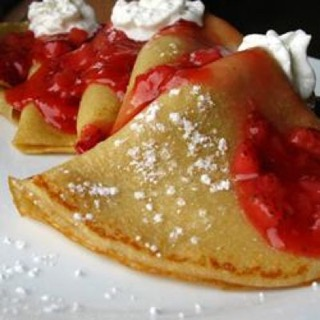
\includegraphics[width=0.9\linewidth]{/home/tim/Documents/projects/recipes/img/FD7839F1-1D5C-4C27-9BA2-0E15CD258A65.jpg}\\
\end{minipage}\vspace{3mm}
\textbf{Directions}:
\vspace{-3mm}\begin{enumerate}\setlength\itemsep{-1mm}
\item In a large mixing bowl, whisk together the flour and the eggs. Gradually add in the milk and water, stirring to combine. Add the salt and butter; beat until smooth.
\item Heat a lightly oiled griddle or frying pan over medium high heat. Pour or scoop the batter onto the griddle, using approximately 1/4 cup for each crepe. Tilt the pan with a circular motion so that the batter coats the surface evenly.
\item Cook the crepe for about 2 minutes, until the bottom is light brown. Loosen with a spatula, turn and cook the other side. Serve hot.
\end{enumerate}
\vspace{2mm}{\Large\textbf{Macadamia Nut Cheesecake}} \label{macadamia-nut-cheesecake}\hfill\textit{}\\
\begin{minipage}[t]{0.8\linewidth}
\textbf{Ingredients}:\vspace{-3mm}
\begin{multicols}{2}
\begin{itemize}\setlength\itemsep{-1mm}
\item 1 3/4 Cups Fine graham cracker crumbs (20 crackers)
\item 1/4 Cup Finely chopped macadamia nuts (may substitute walnuts or pecans)
\item 1/2 tsp Cinnamon
\item 1/2 Cup butter, melted
\item 3 Well beaten eggs
\item 2 Pkgs 8 oz Philadelphia Brand Cream Cheese, soft
\item 1 Cup Sugar
\item 1/4 tsp Salt
\item 2 tsp Vanilla
\item 1/2 tsp almond extract
\item 3 Cups Sour cream
\item 1/4 Cup Finely chopped macadamia nuts (optional)
\item Glaze
\item 1 Pint fresh strawberries
\item 1 Cup Water
\item 1 1/2 Tbsp Cornstarch
\item 1/2 Cup Sugar
\end{itemize}
\end{multicols}
\end{minipage}
\begin{minipage}[t]{0.2\linewidth}
\centering \strut\vspace*{-\baselineskip}\newline
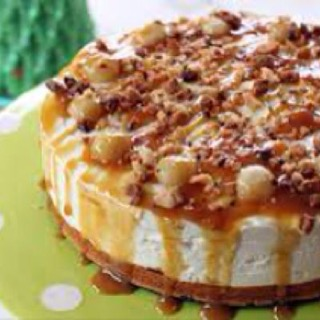
\includegraphics[width=0.9\linewidth]{/home/tim/Documents/projects/recipes/img/89414FEC-14D0-41F8-AE21-0EDCF62611AF.jpg}\\
\end{minipage}\vspace{3mm}
\textbf{Directions}:
\vspace{-3mm}\begin{enumerate}\setlength\itemsep{-1mm}
\item Thoroughly mix ingredients for crust. Press on bottom and sides of 9 inch springform pan. Sides should be about 1 3/4 inches high. Eggs, cream cheese, sugar, salt, vanilla and almond extract. Beat until smooth. Blend in sour cream and nuts. Pour into crumb crust. Bake at 375 about 35 minutes or just until set. Cool. Chill. Thoroughly, about 4 to 5 hours (filling will be soft). 
\item Crush 1 cup strawberries. Add water and cook two minutes. Sieve. Mix cornstarch with sugar and stir into hot berry mixture. Bring to a boil, stirring constantly. Cook and stir until thick and clear (add a few drops of red food coloring if desired). Cool to room temperature. Place remaining strawberries on top of chilled cheesecake. Pour glaze over cake. Chill about 2 hours.
\end{enumerate}
\vspace{2mm}{\Large\textbf{Peanut Butter Brownies}} \label{peanut-butter-brownies}\hfill\textit{}\\
\begin{minipage}[t]{0.8\linewidth}
\textbf{Ingredients}:\vspace{-3mm}
\begin{multicols}{2}
\begin{itemize}\setlength\itemsep{-1mm}
\item 1/2 Cup Sifted flour
\item 1/4 tsp Salt
\item 1/2 Cup Crunchy peanut butter
\item 1/4 Cup Butter
\item 1 tsp vanilla extract
\item 1 Cup Firmly packed brown sugar
\item 2 Eggs
\item 1 Cup Chopped peanuts
\end{itemize}
\end{multicols}
\end{minipage}
\begin{minipage}[t]{0.2\linewidth}
\centering \strut\vspace*{-\baselineskip}\newline
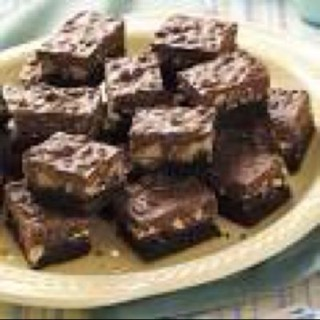
\includegraphics[width=0.9\linewidth]{/home/tim/Documents/projects/recipes/img/CB553CE6-E7C7-4689-91D9-AB2C0915942F.jpg}\\
\end{minipage}\vspace{3mm}
\textbf{Directions}:
\vspace{-3mm}\begin{enumerate}\setlength\itemsep{-1mm}
\item Preheat oven to 350.
\item Sift flour and salt together in a bowl.
\item In a separate bowl, cream peanut butter, butter, and vanilla together; gradually add brown sugar, beating until well blended.
\item Add edges one at a time; beat well after each addition. Blend in flour. Stir in peanuts.
\item Spoon batter into greased, 8-inch square baking pan; spread evenly. Bake for 30-35 minutes, or until center is firm. Cool in pan for 5 minutes, then cut into squares. Remove from pan and cool on wire rack.
\end{enumerate}
\vspace{2mm}{\Large\textbf{Shrimp Alfredo}} \label{shrimp-alfredo}\hfill\textit{Terry Dunn}\\
\begin{minipage}[t]{0.8\linewidth}
\textbf{Ingredients}:\vspace{-3mm}
\begin{multicols}{2}
\begin{itemize}\setlength\itemsep{-1mm}
\item 8 - 12 oz Cream cheese
\item 1 Cup Chicken Broth
\item 2 Tbsp Balsamic vinagrette dressing (terry uses more)
\item 3 Garlic (Cloves)
\item 1 # Shrimp
\end{itemize}
\end{multicols}
\end{minipage}
\begin{minipage}[t]{0.2\linewidth}
\centering \strut\vspace*{-\baselineskip}\newline
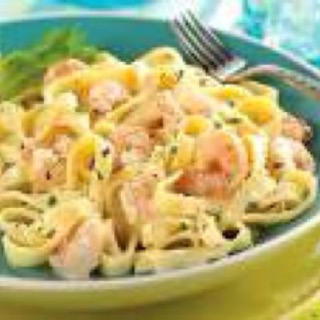
\includegraphics[width=0.9\linewidth]{/home/tim/Documents/projects/recipes/img/9E6506D8-8AA1-42A5-98CD-DCA5194C5531.jpg}\\
\end{minipage}\vspace{3mm}
\textbf{Directions}:
\vspace{-3mm}\begin{enumerate}\setlength\itemsep{-1mm}
\item Saute shrimp in balsamic vinagrette. Add garlic and cook for 3 more minutes. Add more balsamic if desired. Remove shrimp and keep warm. Add broth to same pan, add cream cheese till melted.
\item Serve over fettuccini or pasta
\end{enumerate}
\vspace{2mm}{\Large\textbf{Double Layer Pumpkin Cheesecake}} \label{double-layer-pumpkin-cheesecake}\hfill\textit{}\\
\begin{minipage}[t]{0.8\linewidth}
\textbf{Ingredients}:\vspace{-3mm}
\begin{multicols}{2}
\begin{itemize}\setlength\itemsep{-1mm}
\item 2 pkg cream cheese, softened (8 ounce)
\item 1/2 Cup white sugar
\item 1/2 tsp vanilla extract
\item 2 eggs
\item 1 prepared graham cracker crust (9 inch)
\item 1/2 Cup pumpkin puree
\item 1/2 tsp ground cinnamon
\item 1 pinch ground cloves
\item 1 pinch ground nutmeg
\item 1/2 Cup frozen whipped topping, thawed
\end{itemize}
\end{multicols}
\end{minipage}
\begin{minipage}[t]{0.2\linewidth}
\centering \strut\vspace*{-\baselineskip}\newline
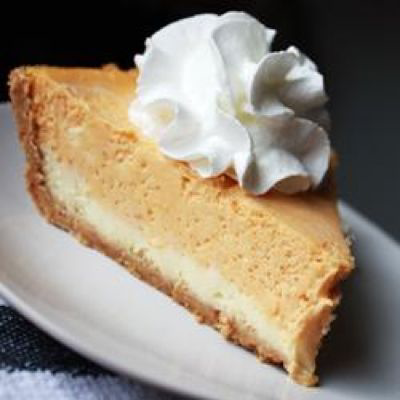
\includegraphics[width=0.9\linewidth]{/home/tim/Documents/projects/recipes/img/E6F502AC-5B4B-4DF3-A847-9DA4B3B3B529.jpg}\\
\end{minipage}\vspace{3mm}
\textbf{Directions}:
\vspace{-3mm}\begin{enumerate}\setlength\itemsep{-1mm}
\item Preheat oven to 325 degrees F (165 degrees C).
\item In a large bowl, combine cream cheese, sugar and vanilla. Beat until smooth. Blend in eggs one at a time. Remove 1 cup of batter and spread into bottom of crust; set aside.
\item Add pumpkin, cinnamon, cloves and nutmeg to the remaining batter and stir gently until well blended. Carefully spread over the batter in the crust.
\item Bake in preheated oven for 35 to 40 minutes, or until center is almost set. Allow to cool, then refrigerate for 3 hours or overnight. Cover with whipped topping before serving.
\end{enumerate}
\vspace{2mm}{\Large\textbf{Island Gem Bars}} \label{island-gem-bars}\hfill\textit{Sue Dunn}\\
\begin{minipage}[t]{0.8\linewidth}
\textbf{Ingredients}:\vspace{-3mm}
\begin{multicols}{2}
\begin{itemize}\setlength\itemsep{-1mm}
\item 1/2 Cup butter, softened
\item 1/2 Cup packed brown sugar
\item 1 tsp Vanilla extract
\item 1 1/2 Cups All-purpose flour
\item 1 Cup packed brown sugar
\item 1/4 Cup All-purpose flour
\item 1/4 tsp Salt
\item 1 tsp Vanilla Extract
\item 2 Large Eggs
\item 1/3 To 1/2 oz. can of flaked sweetened coconut
\item 1 Cup Semisweet Chocolate
\end{itemize}
\end{multicols}
\end{minipage}
\begin{minipage}[t]{0.2\linewidth}
\centering \strut\vspace*{-\baselineskip}\newline
\includegraphics[width=0.9\linewidth]{/home/tim/Documents/projects/recipes/img/}\\
\end{minipage}\vspace{3mm}
\textbf{Directions}:
\vspace{-3mm}\begin{enumerate}\setlength\itemsep{-1mm}
\item Preheat oven to 350 F. Lightly butter a 13x9 baking pan.
\item Cookie Layer: Cream butter, brown sugar, and vanilla with an electric mixer until light. Add flour and blend. Press cookie dough into prepared pan. Bake 10 minutes or until edges are golden brown. Cool on a wire rack. Leave oven on.
\item Coconut Layer: Beat brown sugar, flour, salt, vanilla, and eggs, with an electric mixer. Stir in coconut. Spread over cooled cookie layer. Sprinkle top with chocolate chips. 
\item Bake 20-25 minutes or until edges are golden brown. Cool thoroughly before cutting it into bars.
\end{enumerate}
\vspace{2mm}{\Large\textbf{A Sweeter Variation with Butter}} \label{a-sweeter-variation-with-butter}\hfill\textit{}\\
\begin{minipage}[t]{0.8\linewidth}
\textbf{Ingredients}:\vspace{-3mm}
\begin{multicols}{2}
\begin{itemize}\setlength\itemsep{-1mm}
\item 6 Eggs
\item 1 Cup Butter
\item 2 Cups Sugar
\item 2 tsp Vanilla extract
\item 4 Cups All-purpose flour
\item 3 tsp Baking powder
\end{itemize}
\end{multicols}
\end{minipage}
\begin{minipage}[t]{0.2\linewidth}
\centering \strut\vspace*{-\baselineskip}\newline
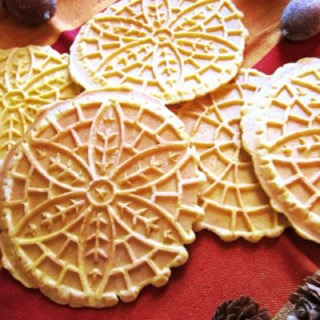
\includegraphics[width=0.9\linewidth]{/home/tim/Documents/projects/recipes/img/FC319651-2B65-4E77-9F33-0858D6C2F97D.jpg}\\
\end{minipage}\vspace{3mm}
\textbf{Directions}:
\vspace{-3mm}\begin{enumerate}\setlength\itemsep{-1mm}
\item Beat the eggs until smooth. Melt the butter and allow to cool briefly while you blend and mix the sugar and vanilla into the eggs. Then add the melted butter into the mix, sift the flour and baking powder onto the mix and blend vigorously to ensure uniformity. The batter will be sticky and stiff. As needed, adjust the mixture with a few tablespoons of water or flour to slightly thin or stiffen the batter so it flows ribbon-like off of a tablespoon.
\item Bake for approximately 20 seconds, opening the lid briefly to examine the color and baking longer as desired to create a darker/browner surface.
\end{enumerate}
\vspace{2mm}{\Large\textbf{Quintessential Veggie Quesadilla}} \label{quintessential-veggie-quesadilla}\hfill\textit{}\\
\begin{minipage}[t]{0.8\linewidth}
\textbf{Ingredients}:\vspace{-3mm}
\begin{multicols}{2}
\begin{itemize}\setlength\itemsep{-1mm}
\item 1/4 Cup carrot, grated
\item 1/4 Cup broccoli, cooked and chopped
\item 1 Tbsp yellow or Vidalia onion, chopped (optional)
\item 1/3 Cup reduced - fat Monterey Jack or Cheddar cheese, shredded
\item 1/2 tsp canola oil
\item 11 - inch flour tortilla (burrito - style)
\item 1 Tbsp salsa or taco sauce
\end{itemize}
\end{multicols}
\end{minipage}
\begin{minipage}[t]{0.2\linewidth}
\centering \strut\vspace*{-\baselineskip}\newline
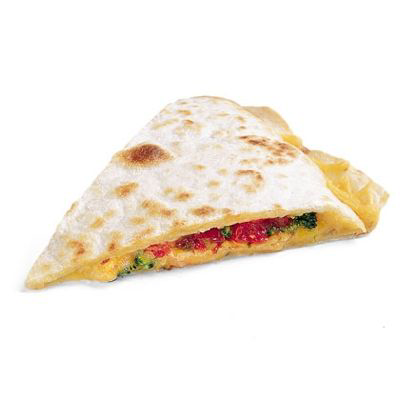
\includegraphics[width=0.9\linewidth]{/home/tim/Documents/projects/recipes/img/87627905-7B4A-4452-B66F-F722F79142DC.jpg}\\
\end{minipage}\vspace{3mm}
\textbf{Directions}:
\vspace{-3mm}\begin{enumerate}\setlength\itemsep{-1mm}
\item In a medium-size bowl, mix together the carrot, broccoli, onion (if desired), and cheese.
\item Set a large nonstick frying pan over medium heat and thinly coat the bottom of the pan with canola oil. Place a tortilla in the pan, cover it with the cheese-veggie mixture, and drizzle the salsa or taco sauce on top.
\item When the bottom of the tortilla is lightly browned and the cheese has melted, fold the quesadilla in half and transfer it to a plate. Cut it into quarters and serve hot. Makes 1 quesadilla.
\end{enumerate}
\vspace{2mm}{\Large\textbf{Torte}} \label{torte}\hfill\textit{Jeanette Keim}\\
\begin{minipage}[t]{0.8\linewidth}
\textbf{Ingredients}:\vspace{-3mm}
\begin{multicols}{2}
\begin{itemize}\setlength\itemsep{-1mm}
\item 6 Egg whites
\item 2 tsp Vanilla
\item 1/2 tsp Cream of tartar
\item Dash salt
\item 2 Cups Sugar
\item 6 English Toffee Bars (Heath) crushed
\item 2 Cups Heavy cream (whipped)
\end{itemize}
\end{multicols}
\end{minipage}
\begin{minipage}[t]{0.2\linewidth}
\centering \strut\vspace*{-\baselineskip}\newline
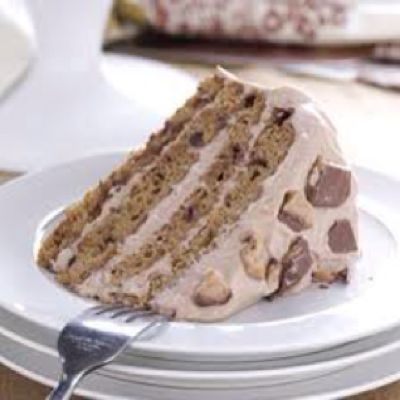
\includegraphics[width=0.9\linewidth]{/home/tim/Documents/projects/recipes/img/0B9EEC9F-6865-4D07-AB33-7CC104026BEA.jpg}\\
\end{minipage}\vspace{3mm}
\textbf{Directions}:
\vspace{-3mm}\begin{enumerate}\setlength\itemsep{-1mm}
\item Have egg whites at room temperature. Add vanilla, cream of tartar and salt. Beat to soft peaks, gradually add sugar and beat to stiff peaks. Cut two 9'' circles of brown paper (grocery bags), place on the cookie sheets and cover each with half the meringue mixture. Bake at 275 for 1 hour then let cool in oven (overnight works well). Combine whipped cream and crushed toffee bars. Spread half between meringue layers and half on top. Let chil in fridge at least 8 hours. Hint: Freeze Heath bars and they will be easier to crush.
\end{enumerate}
\vspace{2mm}{\Large\textbf{Dark Chocolate Truffles}} \label{dark-chocolate-truffles}\hfill\textit{}\\
\begin{minipage}[t]{0.8\linewidth}
\textbf{Ingredients}:\vspace{-3mm}
\begin{multicols}{2}
\begin{itemize}\setlength\itemsep{-1mm}
\item 1 3/4 Cups Ghirardelli 60 Cacao Bittersweet Chocolate Baking Chips
\item 1/3 Cup Ghirardelli Unsweetened Cocoa
\item 1/3 Cup heavy whipping cream
\item 6 Tbsp unsalted butter, cut into small pieces
\end{itemize}
\end{multicols}
\end{minipage}
\begin{minipage}[t]{0.2\linewidth}
\centering \strut\vspace*{-\baselineskip}\newline
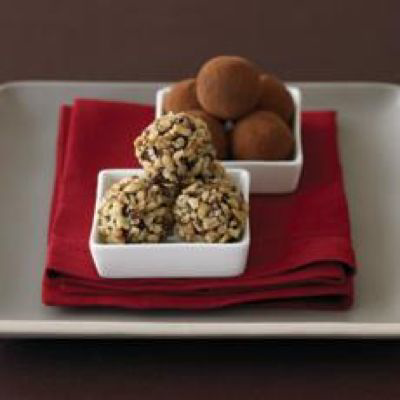
\includegraphics[width=0.9\linewidth]{/home/tim/Documents/projects/recipes/img/C5CA061F-9F08-4AF1-9D07-BF6A9B12CCA6.jpg}\\
\end{minipage}\vspace{3mm}
\textbf{Directions}:
\vspace{-3mm}\begin{enumerate}\setlength\itemsep{-1mm}
\item Directions
\item In a small saucepan, bring the cream to a simmer. Add the butter and stir until melted. Add the chocolate chips. Stir until completely melted and smooth. Remove from the heat and pour into a shallow bowl.
\item Cool, cover, and refrigerate the mixture until firm, at least 2 hours.
\item Using a melon baller or small spoon, roll the mixture into 1-inch balls. Roll each ball in the cocoa. Enjoy immediately or refrigerate in an airtight container for up to 2 weeks.
\item Note: The Unsweetened Cocoa can be replaced with 3/4 cup of chopped almonds or pecans.
\end{enumerate}
\vspace{2mm}{\Large\textbf{Magic Cookie Bars}} \label{magic-cookie-bars}\hfill\textit{}\\
\begin{minipage}[t]{0.8\linewidth}
\textbf{Ingredients}:\vspace{-3mm}
\begin{multicols}{2}
\begin{itemize}\setlength\itemsep{-1mm}
\item 2 Cups Ghirardelli Semi - Sweet Chocolate Chips
\item 1/2 Cup butter or margarine
\item 1 1/2 Cups graham cracker crumbs
\item 14 oz fluid sweetened condensed milk (NOT evaporated milk)
\item 1 1/3 Cups flaked coconut
\item 1 Cup chopped nuts
\end{itemize}
\end{multicols}
\end{minipage}
\begin{minipage}[t]{0.2\linewidth}
\centering \strut\vspace*{-\baselineskip}\newline
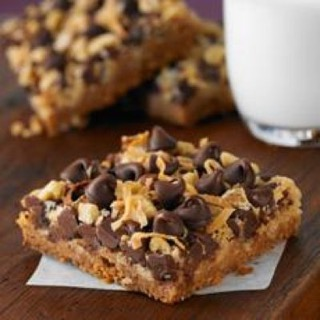
\includegraphics[width=0.9\linewidth]{/home/tim/Documents/projects/recipes/img/5B628267-AAB3-450D-934D-051D2010227C.jpg}\\
\end{minipage}\vspace{3mm}
\textbf{Directions}:
\vspace{-3mm}\begin{enumerate}\setlength\itemsep{-1mm}
\item Preheat oven to 350F (325F for glass dish). In 13" x 9" baking pan, melt butter in oven. Sprinkle crumbs over butter; pour sweetened condensed milk evenly over crumbs. Top with remaining ingredients; press down firmly with fork. Bake 25 minutes or until lightly browned.
\item Cool. Chill if desired. Cut into bars. Store covered at room temperature.
\end{enumerate}
\vspace{2mm}{\Large\textbf{Gooey Butterscotch Bars Recipe}} \label{gooey-butterscotch-bars-recipe}\hfill\textit{}\\
\begin{minipage}[t]{0.8\linewidth}
\textbf{Ingredients}:\vspace{-3mm}
\begin{multicols}{2}
\begin{itemize}\setlength\itemsep{-1mm}
\item 1 pkg sugar cookie mix (17 1/2 ounces)
\item 1 pkg instant butterscotch pudding mix (3.4 ounces)
\item 1/2 Cup butter, softened
\item 1 egg
\item 14 oz caramels
\item 1/2 Cup evaporated milk
\item 2 Cups mixed nuts
\item 1 tsp vanilla extract
\item 1 Cup butterscotch chips
\end{itemize}
\end{multicols}
\end{minipage}
\begin{minipage}[t]{0.2\linewidth}
\centering \strut\vspace*{-\baselineskip}\newline
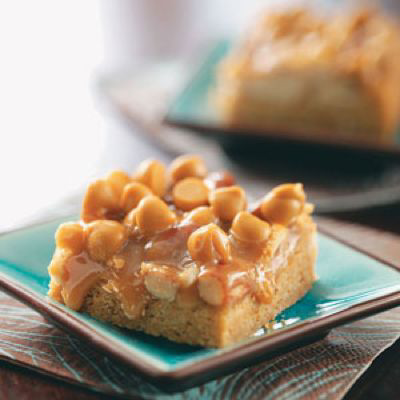
\includegraphics[width=0.9\linewidth]{/home/tim/Documents/projects/recipes/img/A68016B2-4669-442D-B384-D6A042141E05.jpg}\\
\end{minipage}\vspace{3mm}
\textbf{Directions}:
\vspace{-3mm}\begin{enumerate}\setlength\itemsep{-1mm}
\item In a large bowl, combine the sugar cookie mix, pudding mix, butter and egg. Press into an ungreased 13-in. x 9-in. baking pan. Bake at 350&deg< for 20-25 minutes or until set. 
\item  In a large saucepan, combine caramels and milk. Cook and stir over medium-low heat until melted. Remove from the heat. Stir in nuts and vanilla. Pour over crust. Sprinkle with butterscotch chips. 
\item  Cool completely. Cut into bars. Store in an airtight container. Yield: about 3 dozen.
\end{enumerate}
\vspace{2mm}{\Large\textbf{Broccoli, Cheddar and Ham Strata}} \label{broccoli,-cheddar-and-ham-strata}\hfill\textit{}\\
\begin{minipage}[t]{0.8\linewidth}
\textbf{Ingredients}:\vspace{-3mm}
\begin{multicols}{2}
\begin{itemize}\setlength\itemsep{-1mm}
\item 1 tsp Olive Oil
\item 1 Medium Onion (Diced)
\item 16 oz Bag of thawed chopped broccoli
\item 1 Loaf Italian Bread (14 oz.) but into cubes
\item 1/2 lb Sliced low-sodium deli ham, chopped
\item 6 Large Eggs
\item 1 1/2 Cups Milk
\item 2 tsp Chives
\item 1 tsp Dijon Mustard
\item 1/2 tsp Salt
\item 1/4 tsp pepper
\item 1 1/2 Cups shredded Cheddar cheese
\end{itemize}
\end{multicols}
\end{minipage}
\begin{minipage}[t]{0.2\linewidth}
\centering \strut\vspace*{-\baselineskip}\newline
\includegraphics[width=0.9\linewidth]{/home/tim/Documents/projects/recipes/img/}\\
\end{minipage}\vspace{3mm}
\textbf{Directions}:
\vspace{-3mm}\begin{enumerate}\setlength\itemsep{-1mm}
\item Heat oven to 375. Coat 2 quart oval baking sheet dish with nonstick spray
\item Heat oil in a large nonstick skillet over medium heat. Add onion and cook 5 minutes. Add broccoli and cook another 3 minutes.
\item Place bread cubes in a large bowl. Stir in onion and broccoli mixture and the ham. 
\item In a medium bowl, whick together eggs, milk, chives, mustard, salt and pepper. Pour over great mixture, stirring to mix. Transfer to prepared dish, and top evenly with cheese. 
\item Bake at 375 for 40-45 minutes, or until strata registers 160 on thermometer.
\end{enumerate}
\vspace{2mm}{\Large\textbf{Guiltless Alfredo sauce}} \label{guiltless-alfredo-sauce}\hfill\textit{}\\
\begin{minipage}[t]{0.8\linewidth}
\textbf{Ingredients}:\vspace{-3mm}
\begin{multicols}{2}
\begin{itemize}\setlength\itemsep{-1mm}
\item 3 oz reduced - fat cream cheese , softened (Neufch tel)
\item 2 Cups Low fat milk
\item 1 Tbsp butter
\item 1 tsp Salt
\item 2 1/2 Tbsp Flour
\item 3 cloves garlic, finely chopped
\item 1 Cup grated Parmesan cheese
\end{itemize}
\end{multicols}
\end{minipage}
\begin{minipage}[t]{0.2\linewidth}
\centering \strut\vspace*{-\baselineskip}\newline
\includegraphics[width=0.9\linewidth]{/home/tim/Documents/projects/recipes/img/}\\
\end{minipage}\vspace{3mm}
\textbf{Directions}:
\vspace{-3mm}\begin{enumerate}\setlength\itemsep{-1mm}
\item Blend cream cheese, milk, flour and salt until smooth
\item Melt butter in sauce pan and saute garlic for 1 minute
\item Add milk mixture to sauce burn and cook to simmer for 5 minutes
\item Remove from heat, add cheese, stir and cover for 10 minutes
\end{enumerate}
\vspace{2mm}{\Large\textbf{Banana Bread}} \label{banana-bread}\hfill\textit{Alpha Bakery Children's Book}\\
\begin{minipage}[t]{0.8\linewidth}
\textbf{Ingredients}:\vspace{-3mm}
\begin{multicols}{2}
\begin{itemize}\setlength\itemsep{-1mm}
\item 3/4 Cup Sugar
\item 1 1/2 Cups Mashed bananas (3 large)
\item 3/4 Cup Vegetable Oil
\item 2 Eggs
\item 2 Cups all - purpose flour
\item 1/2 Cup chocolate chips (or nuts)
\item 1 tsp Baking soda
\item 2 tsp Vanilla
\item 1/2 tsp Baking powder
\item 1/2 tsp Salt
\end{itemize}
\end{multicols}
\end{minipage}
\begin{minipage}[t]{0.2\linewidth}
\centering \strut\vspace*{-\baselineskip}\newline
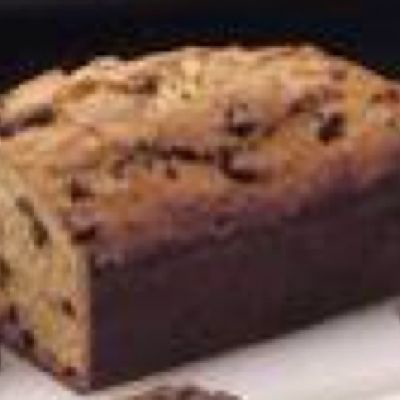
\includegraphics[width=0.9\linewidth]{/home/tim/Documents/projects/recipes/img/A1DC5656-FAA8-460B-9E34-05D4EEAB7F19.jpg}\\
\end{minipage}\vspace{3mm}
\textbf{Directions}:
\vspace{-3mm}\begin{enumerate}\setlength\itemsep{-1mm}
\item Heat the oven to 350.
\item Grease a loaf pan, either 9x5x3 or 8 1/2 x4 1/2 x2 1/2 inches, with shortening, using a pastry brush.
\item Mix sugar, bananas, oil and eggs in a large bowl with a wooden spoon. Stir in remaining ingredients. Pour into pan.
\item Bake until a wooden pick inserted in the center of the bread comes out clean (60-70 minutes). Let cool 10 minutes, then loosen sides of loaf from pan and remove from pan. Let cool completely before slicing. 
\end{enumerate}
\vspace{2mm}{\Large\textbf{White Thin Mints}} \label{white-thin-mints}\hfill\textit{}\\
\begin{minipage}[t]{0.8\linewidth}
\textbf{Ingredients}:\vspace{-3mm}
\begin{multicols}{2}
\begin{itemize}\setlength\itemsep{-1mm}
\item 1 Box Vanilla Wafer Cookies (such as Nilla Wafers)
\item 2 Cups mint white chocolate candy melts
\item Sprinkles (optional)
\end{itemize}
\end{multicols}
\end{minipage}
\begin{minipage}[t]{0.2\linewidth}
\centering \strut\vspace*{-\baselineskip}\newline
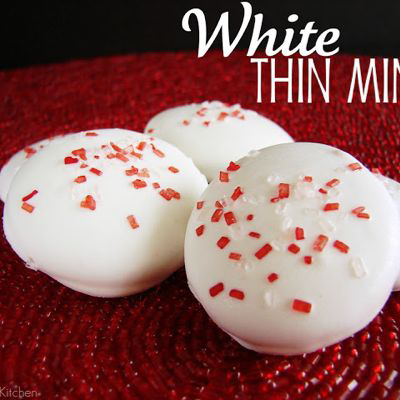
\includegraphics[width=0.9\linewidth]{/home/tim/Documents/projects/recipes/img/98E9104A-8DEE-4B51-8465-C4ADE77BF39B.jpg}\\
\end{minipage}\vspace{3mm}
\textbf{Directions}:
\vspace{-3mm}\begin{enumerate}\setlength\itemsep{-1mm}
\item Melt chocolate in microwave (Use about 1 Tablespoon shortening or vegetable oil to thin it out if it is too think for dipping.)
\item Dip cookies into mint white chocolate. Garnish with sprinkles if desired. Let cool.
\item You can find mint white chocolate at most craft/baking supply stores (JoAnne's, Pat Catan's, Michaels).
\item You can substitute regular white chocolate with about 1/2 teaspoon peppermint extract.
\end{enumerate}
\vspace{2mm}{\Large\textbf{Chocolate Malted Milkshake}} \label{chocolate-malted-milkshake}\hfill\textit{}\\
\begin{minipage}[t]{0.8\linewidth}
\textbf{Ingredients}:\vspace{-3mm}
\begin{multicols}{2}
\begin{itemize}\setlength\itemsep{-1mm}
\item 2 1/2 Cups chocolate ice cream
\item 1/2 Cup original flavor malted milk powder
\item 1/2 Cup whole milk
\item Sweetened whipped cream, for garnish
\item Halved malted milk balls, for garnish
\end{itemize}
\end{multicols}
\end{minipage}
\begin{minipage}[t]{0.2\linewidth}
\centering \strut\vspace*{-\baselineskip}\newline
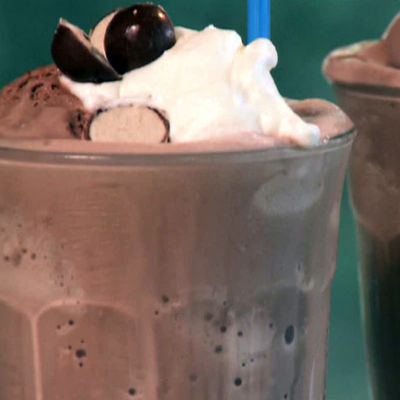
\includegraphics[width=0.9\linewidth]{/home/tim/Documents/projects/recipes/img/985FB684-E2F9-41F7-81E5-667147B22559.jpg}\\
\end{minipage}\vspace{3mm}
\textbf{Directions}:
\vspace{-3mm}\begin{enumerate}\setlength\itemsep{-1mm}
\item  In the container of a blender, combine the ice cream and malted milk powder. Add the milk, a quarter cup at a time, blending between each addition, until the desired consistency is reached. Garnish with whipped cream and malted milk balls. 
\end{enumerate}
\vspace{2mm}{\Large\textbf{Pumpkin Waffles}} \label{pumpkin-waffles}\hfill\textit{Carolyn Benjamin}\\
\begin{minipage}[t]{0.8\linewidth}
\textbf{Ingredients}:\vspace{-3mm}
\begin{multicols}{2}
\begin{itemize}\setlength\itemsep{-1mm}
\item 1 Cup Flour
\item 2 tsp Baking powder
\item 3/4 tsp Ground Cinnamon
\item 1/8 tsp Ground cloves
\item 1 Cup Low fat milk
\item 1/2 Cup Pumpkin puree
\item 1/4 Cup Packed Dark Brown Sugar
\item 1 Tbsp vegetable oil
\item 1 Large Egg, slightly beaten
\end{itemize}
\end{multicols}
\end{minipage}
\begin{minipage}[t]{0.2\linewidth}
\centering \strut\vspace*{-\baselineskip}\newline
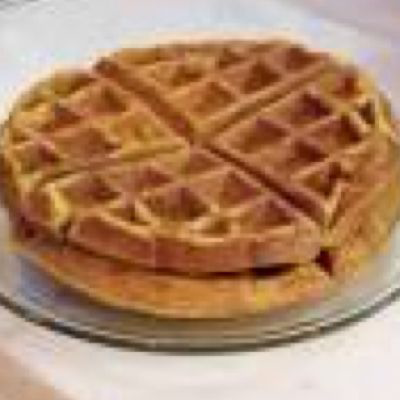
\includegraphics[width=0.9\linewidth]{/home/tim/Documents/projects/recipes/img/6F6656B5-56C4-49D2-A435-402CEA169684.jpg}\\
\end{minipage}\vspace{3mm}
\textbf{Directions}:
\vspace{-3mm}\begin{enumerate}\setlength\itemsep{-1mm}
\item Spoon flour into measuring cup and level with a knife
\item Combine flour and next 4 ingredients (through cloves) in a large bowl.
\item Make a well in the center of the mixture
\item Combine milk and next 4 ingredients (through egg) in a bowl and add flour mixture. Stir until moist.
\item Coat waffle iron with cooking spray (if necessary). Spoon about 1/4 cup batter per waffle into hot waffle iron spreading batter to edges
\end{enumerate}
\vspace{2mm}{\Large\textbf{Monster Cookies}} \label{monster-cookies}\hfill\textit{Carolyn benjamin}\\
\begin{minipage}[t]{0.8\linewidth}
\textbf{Ingredients}:\vspace{-3mm}
\begin{multicols}{2}
\begin{itemize}\setlength\itemsep{-1mm}
\item 3 Eggs
\item 1 Cup Brown Sugar
\item 3/4 tsp Vanilla
\item 1 Cup Granulated Sugar
\item 2 tsp Baking Soda
\item 1/2 Cup Butter
\item 2 Cups Peanut Butter
\item 4 1/2 Cups Oatmeal
\item 1/2 Cup Chocolate Chips (Chocolate Chunks)
\item 1/2 Cup M&Ms
\item 1/8 Cup Chopped Nuts
\end{itemize}
\end{multicols}
\end{minipage}
\begin{minipage}[t]{0.2\linewidth}
\centering \strut\vspace*{-\baselineskip}\newline
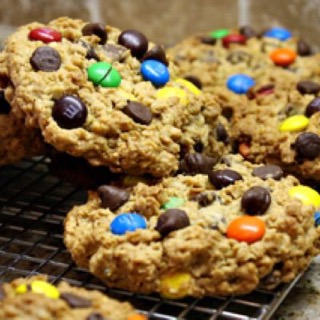
\includegraphics[width=0.9\linewidth]{/home/tim/Documents/projects/recipes/img/338BA54A-1A96-4D53-B39E-7AD0183F00F2.jpg}\\
\end{minipage}\vspace{3mm}
\textbf{Directions}:
\vspace{-3mm}\begin{enumerate}\setlength\itemsep{-1mm}
\item Combine all ingredients. Use an ice cream scoop to form balls of dough, then gently flatten dough on cookie sheet. Bake at 350 for 10-12 minutes.
\end{enumerate}
\vspace{2mm}{\Large\textbf{Dark Chocolate Cupcakes}} \label{dark-chocolate-cupcakes}\hfill\textit{}\\
\begin{minipage}[t]{0.8\linewidth}
\textbf{Ingredients}:\vspace{-3mm}
\begin{multicols}{2}
\begin{itemize}\setlength\itemsep{-1mm}
\item 1/4 Cup Ghirardelli Unsweetened Cocoa
\item 1 1/8 Cups all - purpose flour
\item 1 1/4 tsp baking soda
\item 1/4 tsp salt
\item 1 Large egg
\item 1/2 Cup firmly packed light brown sugar
\item 1/2 Cup granulated white sugar
\item 5/8 Cup whole milk
\item 1/3 Cup strong brewed coffee or espresso
\item 1/2 Cup unsalted butter (or 1 stick)
\end{itemize}
\end{multicols}
\end{minipage}
\begin{minipage}[t]{0.2\linewidth}
\centering \strut\vspace*{-\baselineskip}\newline

\includegraphics[width=0.9\linewidth]{/home/tim/Documents/projects/recipes/img/E13D67A0-124A-47A0-B785-EF3D82D6CF1D.jpg}\\
\end{minipage}\vspace{3mm}
\textbf{Directions}:
\vspace{-3mm}\begin{enumerate}\setlength\itemsep{-1mm}
\item Preheat the oven to 350F. Line 12 cupcake molds or muffin tins with paper liners or spray with nonstick spray. To make the cupcakes, sift together the flour, cocoa, baking soda and salt. In a medium bowl, whisk together the egg, brown sugar, and white sugar. Whisk in the milk, coffee, and melted butter. Whisk in the dry ingredients. Divide the batter evenly among the cupcake molds, filling them about three-quarters full.
\item Bake for 15 minutes, or until a tester inserted in the middle of the cupcakes comes out clean. Cool for 10 minutes. Using a small spatula or knife, remove the cupcakes from the pan. Continue to cool on a wire rack to room temperature.
\item To make the frosting, melt the chopped chocolate in the top of a double boiler, or in a heatproof bowl, over barely simmering water, stirring occasionally until smooth. Heat the cream until hot. Remove from the heat and whisk in the chocolate. Transfer to a bowl and cool to just warm. Whisk in the butter until smooth. Let sit until it reaches a spreading consistency, about 1 hour. Spread the frosting on top of the cupcakes. Sprinkle them with chocolate chips.
\end{enumerate}
\vspace{2mm}{\Large\textbf{Honey Balasamic Salmon}} \label{honey-balasamic-salmon}\hfill\textit{}\\
\begin{minipage}[t]{0.8\linewidth}
\textbf{Ingredients}:\vspace{-3mm}
\begin{multicols}{2}
\begin{itemize}\setlength\itemsep{-1mm}
\item 1 Spray(s) cooking spray
\item 1/4 tsp Olive Oil
\item 1/2 Cup Leek(s), julienne-cut (about 1 small)
\item 1 1/2 lb Salmon fillets, with or without skin, four 6-oz. pieces
\item 1/2 tsp Table salt, divided
\item 1/4 tsp Black pepper, divided
\item 1/2 Cup Balsamic vinegar
\item 1 Tbsp Honey
\end{itemize}
\end{multicols}
\end{minipage}
\begin{minipage}[t]{0.2\linewidth}
\centering \strut\vspace*{-\baselineskip}\newline

\includegraphics[width=0.9\linewidth]{/home/tim/Documents/projects/recipes/img/53AC6E19-DE06-4A08-87E0-2EBE21E19FB6.jpg}\\
\end{minipage}\vspace{3mm}
\textbf{Directions}:
\vspace{-3mm}\begin{enumerate}\setlength\itemsep{-1mm}
\item Coat a large nonstick skillet with cooking spray; add oil. Place over medium-high heat; add leaks and saute 3 to 4 minutes or until soft. Remove from pan and set aside.
\item Sprinkle fish with 1/4 tsp salt and 1/8 tsp pepper. Add fish to pan; cook 3 to 4 minutes on each side or until lightly browned and fish flakes easily when tested with a fork. Remove from pan; set aside, and keep warm.
\item Add vinegar, honey, 1/4 tsp salt, and 1/8 tsp pepper to pan. Cook over medium-high heat 3-4 minutes or until reduced by half. Divide leaks evenly over fish; drizzle with sauce. 
\end{enumerate}
\vspace{2mm}{\Large\textbf{Beef Chili}} \label{beef-chili}\hfill\textit{}\\
\begin{minipage}[t]{0.8\linewidth}
\textbf{Ingredients}:\vspace{-3mm}
\begin{multicols}{2}
\begin{itemize}\setlength\itemsep{-1mm}
\item 1 Tbsp Wegmans Vegetable Oil
\item 3 lb 90 Lean Ground Beef
\item Salt
\item 2 pkg Food You Feel Good About Cleaned & Cut Chopped Onions (8 oz each)
\item 1 pkg Food You Feel Good About Diced Green Peppers and Onions (8 oz)
\item 3 cloves Food You Feel Good About Peeled Garlic, minced
\item 4 Tbsp Worcestershire sauce
\item 7 Tbsp chili powder (about 2 oz)
\item 2 tsp ground cumin
\item 2 tsp oregano
\item 1 Can Wegmans Dark Red Kidney Beans, drained and rinsed (15.5 oz)
\item 1 Can Italian Classics Cannellini Beans, drained and rinsed (15.5 oz)
\item 2 btls Wegmans Chili Sauce (12 oz each)
\item 1 Cup bottle beer or 1 1/2 Food You Feel Good About Beef Culinary Stock (12 oz)
\end{itemize}
\end{multicols}
\end{minipage}
\begin{minipage}[t]{0.2\linewidth}
\centering \strut\vspace*{-\baselineskip}\newline
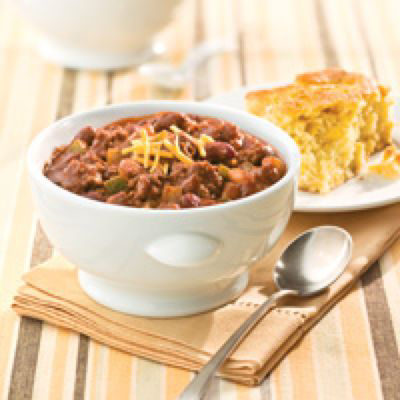
\includegraphics[width=0.9\linewidth]{/home/tim/Documents/projects/recipes/img/8E97E9A3-9433-46A8-BFFA-12F2EC36BBB9.jpg}\\
\end{minipage}\vspace{3mm}
\textbf{Directions}:
\vspace{-3mm}\begin{enumerate}\setlength\itemsep{-1mm}
\item Heat vegetable oil on MEDIUM-HIGH. Add ground beef; cook 8-10 min until browned. Season with salt.
\item Add chopped onions, green peppers, and garlic. Cook, stirring, 3-5 min. Add Worcestershire sauce; cook 3 min.
\item Reduce heat to MEDIUM; stir in chili powder, cumin, and oregano. Cook 5 min. Reduce heat to LOW; add kidney beans, cannellini beans, chili sauce, and beer (or stock). Simmer 30 min, stirring occasionally.
\item Option(s):
\item Garnish with cheddar cheese.
\end{enumerate}
\vspace{2mm}{\Large\textbf{Sesame Chicken with Lo Mein & Green Beans}} \label{sesame-chicken-with-lo-mein-&-green-beans}\hfill\textit{}\\
\begin{minipage}[t]{0.8\linewidth}
\textbf{Ingredients}:\vspace{-3mm}
\begin{multicols}{2}
\begin{itemize}\setlength\itemsep{-1mm}
\item 1 pkg Food You Feel Good About Cleaned & Cut Trimmed Green Beans (12 oz)
\item 1 pkg box Asian Classics Lo Mein Noodles (Frozen Foods), thawed per directions (16 oz)
\item 1 lb Wegmans Seasoned Chicken Breast Strips for Stir - Fry
\item 3 Tbsp Wegmans Vegetable Oil, divided
\item 2 cloves Food You Feel Good About Cleaned & Cut Peeled Garlic, minced
\item 1 pkg Food You Feel Good About Cleaned & Cut Asian Slaw (12 oz)
\item Salt and pepper to taste
\item 1 Cup Asian Classics Sesame Garlic Sauce (International Foods)
\item 1 Tbsp JFC White Roasted Sesame Seeds (International Foods)
\end{itemize}
\end{multicols}
\end{minipage}
\begin{minipage}[t]{0.2\linewidth}
\centering \strut\vspace*{-\baselineskip}\newline
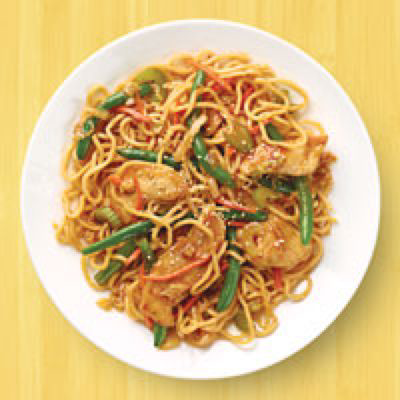
\includegraphics[width=0.9\linewidth]{/home/tim/Documents/projects/recipes/img/C4DA5C56-7DBC-45AD-B917-30CD2579C7C2.jpg}\\
\end{minipage}\vspace{3mm}
\textbf{Directions}:
\vspace{-3mm}\begin{enumerate}\setlength\itemsep{-1mm}
\item Blanch green beans in large pot of boiling salted water 3-4 min. Remove beans with slotted spoon; drain and set aside. Add noodles to blanching water; blanch 2 min. Drain and set aside.
\item Drizzle 2 Tbsp oil around sides of stir-fry pan; tilt pan to distribute evenly. Heat oil in pan on HIGH until oil faintly smokes. (If oil smokes too much, pan is too hot.) Stir fry chicken 4-5 min; remove from pan and set aside. 
\item Drizzle remaining Tbsp oil around sides of pan; tilt pan to distribute evenly. Heat oil in pan on HIGH until oil faintly smokes. Add garlic, Asian slaw, and green beans. Stir and toss, 2-3 min. Season to taste with salt and pepper.
\item Add chicken, noodles, and sesame garlic sauce to stir-fry pan. Stir briefly to heat through, 2-3 min. Garnish with sesame seeds.
\end{enumerate}
\vspace{2mm}{\Large\textbf{Seven Layer Taco Dip}} \label{seven-layer-taco-dip}\hfill\textit{allrecipes.com}\\
\begin{minipage}[t]{0.8\linewidth}
\textbf{Ingredients}:\vspace{-3mm}
\begin{multicols}{2}
\begin{itemize}\setlength\itemsep{-1mm}
\item 1 pkg taco seasoning mix (1 ounce)
\item 1 Can refried beans (16 ounce)
\item 1 pkg cream cheese, softened (8 ounce)
\item 1 container sour cream (16 ounce)
\item 1 jar salsa (16 ounce)
\item 1 Large tomato, chopped
\item 1 green bell pepper, chopped
\item 1 bunch chopped green onions
\item 1 Small head iceberg lettuce, shredded
\item 1 Can sliced black olives, drained (6 ounce)
\item 2 Cups shredded Cheddar cheese
\end{itemize}
\end{multicols}
\end{minipage}
\begin{minipage}[t]{0.2\linewidth}
\centering \strut\vspace*{-\baselineskip}\newline
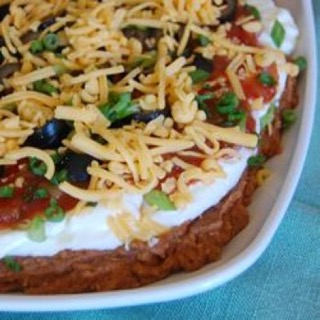
\includegraphics[width=0.9\linewidth]{/home/tim/Documents/projects/recipes/img/7F6379BA-8535-4AB3-A2A2-E1B87DEABB24.jpg}\\
\end{minipage}\vspace{3mm}
\textbf{Directions}:
\vspace{-3mm}\begin{enumerate}\setlength\itemsep{-1mm}
\item In a medium bowl, blend the taco seasoning mix and refried beans. Spread the mixture onto a large serving platter.
\item Mix the sour cream and cream cheese in a medium bowl. Spread over the refried beans.
\item Top the layers with salsa. Place a layer of tomato, green bell pepper, green onions and lettuce over the salsa, and top with Cheddar cheese. Garnish with black olives.
\end{enumerate}
\vspace{2mm}{\Large\textbf{Nutella-Stuffed Brown Butter + Sea Salt Chocolate Chip Cookies}} \label{nutella-stuffed-brown-butter-+-sea-salt-chocolate-chip-cookies}\hfill\textit{}\\
\begin{minipage}[t]{0.8\linewidth}
\textbf{Ingredients}:\vspace{-3mm}
\begin{multicols}{2}
\begin{itemize}\setlength\itemsep{-1mm}
\item 2 1/4 Cups all - purpose flour
\item 1 1/4 tsp baking soda
\item 1/4 tsp of salt
\item 2 sticks unsalted butter (1 cup)
\item 1 1/4 Cups packed dark brown sugar
\item 1/4 Cup granulated sugar
\item 1 Large egg plus 1 egg yolk
\item 1 1/2 tsp vanilla extract
\item 1 Tbsp plain greek yogurt
\item 3/4 Cup semi - sweet chocolate chips
\item 1/2 Cup milk chocolate chips
\item 1/2 Cup dark chocolate chips
\item 1 jar of Nutella, chilled in refrigerator
\item Coarse sea salt for sprinkling
\end{itemize}
\end{multicols}
\end{minipage}
\begin{minipage}[t]{0.2\linewidth}
\centering \strut\vspace*{-\baselineskip}\newline
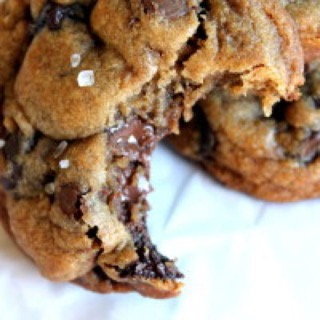
\includegraphics[width=0.9\linewidth]{/home/tim/Documents/projects/recipes/img/35973F0A-56A0-4A47-82FA-7F4291CEF3C9.jpg}\\
\end{minipage}\vspace{3mm}
\textbf{Directions}:
\vspace{-3mm}\begin{enumerate}\setlength\itemsep{-1mm}
\item Whisk together the flour, baking soda, and salt in a bowl and set aside. Melt butter in a saucepan over medium heat. The butter will begin to foam. Make sure you whisk consistently during this process. After a couple of minutes, the butter will begin to brown on the bottom of the saucepan; continue to whisk and remove from heat as soon as the butter begins to brown and give off a nutty aroma. Immediately transfer the butter to a bowl to prevent burning. Set aside to cool for a few minutes.
\item With an electric mixer, mix the butter and sugars until thoroughly blended. Beat in the egg, yolk, vanilla, and yogurt until combined. Add the dry ingredients slowly and beat on low-speed just until combined. Gently fold in all of the chocolate chips.
\item Chill your dough for 2 hours in the refrigerator, or place in freezer for 30 minutes if you are super eager, although I cannot promise the same results if you do this.
\item Preheat the oven to 350 degrees F. Once dough is chilled measure about 1 1/2 tablespoons of dough and roll into a ball. Flatten the dough ball very thinly into the palm of your hand. Place 1 teaspoon of chilled nutella in the middle and fold dough around it; gently roll into a ball - it doesnt have to be perfectly rolled! Make sure that the nutella is not seeping out of the dough. Add more dough if necessary. Place dough balls on cookie sheet, 2 inches apart and flatten with your hand VERY gently. (Really only the tops need to be flattened a bit!)
\item Bake the cookies 9-11 minutes or until the edges of the cookies begin to turn golden brown. They will look a bit underdone in the middle, but will continue to cook once out of the oven. Cool the cookies on the sheets at least 2 minutes. Sprinkle with a little sea salt. Remove the cooled cookies from the baking sheets after a few minutes and transfer to a wire rack to cool completely. Repeat with remaining dough.
\end{enumerate}
\vspace{2mm}{\Large\textbf{Ham and Egg Casserole}} \label{ham-and-egg-casserole}\hfill\textit{}\\
\begin{minipage}[t]{0.8\linewidth}
\textbf{Ingredients}:\vspace{-3mm}
\begin{multicols}{2}
\begin{itemize}\setlength\itemsep{-1mm}
\item 12 Small slices white bread, crusts removed, torn into pieces
\item 3 Cups cooked, cubed ham
\item 3 Cups chopped frozen broccoli, thawed
\item 8 oz shredded sharp Cheddar cheese
\item 0.5 Cup milk
\item 6 eggs, beaten
\item 1 1/4 tsp salt
\item 1 tsp dry mustard
\item tablespoons melted butter
\end{itemize}
\end{multicols}
\end{minipage}
\begin{minipage}[t]{0.2\linewidth}
\centering \strut\vspace*{-\baselineskip}\newline
\includegraphics[width=0.9\linewidth]{/home/tim/Documents/projects/recipes/img/D08AE61F-C771-49C4-8DD1-111FCF4EA38E.jpg}\\
\end{minipage}\vspace{3mm}
\textbf{Directions}:
\vspace{-3mm}\begin{enumerate}\setlength\itemsep{-1mm}
\item In a 9x13x2-inch baking dish, put enough of the bread pieces into the bottom of the pan to make a thin layer. Make a layer of ham, broccoli, and cheese. Whisk together milk, eggs, salt, and dry mustard. Pour over top. Toss remaining bread with butter; sprinkle over the top of the casserole. Bake at 325 for 45 minutes. Let cool for about 20 minutes; cut into squares. Serves 10 to 12.
\end{enumerate}
\vspace{2mm}{\Large\textbf{Butterscotch Brownies}} \label{butterscotch-brownies}\hfill\textit{}\\
\begin{minipage}[t]{0.8\linewidth}
\textbf{Ingredients}:\vspace{-3mm}
\begin{multicols}{2}
\begin{itemize}\setlength\itemsep{-1mm}
\item 1/4 Cup Butter
\item 1 Cup packed light brown sugar
\item 1 Egg
\item 1/2 Cup Sifted flour
\item 1 tsp baking powder
\item 1/2 tsp Salt
\item 1/2 tsp vanilla extract
\item 1/2 Cup chopped walnuts or chocolate chips
\end{itemize}
\end{multicols}
\end{minipage}
\begin{minipage}[t]{0.2\linewidth}
\centering \strut\vspace*{-\baselineskip}\newline
\includegraphics[width=0.9\linewidth]{/home/tim/Documents/projects/recipes/img/67444E5C-1EB3-4B88-BD8B-1497D7DBD3F0.jpg}\\
\end{minipage}\vspace{3mm}
\textbf{Directions}:
\vspace{-3mm}\begin{enumerate}\setlength\itemsep{-1mm}
\item Preheat oven to 350. 
\item Melt butter in saucepan over low heat. Remove from heat; stir in sugar. Mix until well blended; cool. Stir in egg.
\item Sift flour, baking powder, and salt together in bowl. Add to butter mixture; blend well. Stir in vanilla and walnuts.
\item Pour batter into greased and floured, 8-inch square pan. Bake for 20-35 minutes. Cut into squares while still warm.
\end{enumerate}
\vspace{2mm}{\Large\textbf{Sweet Potatoes Mashed}} \label{sweet-potatoes-mashed}\hfill\textit{}\\
\begin{minipage}[t]{0.8\linewidth}
\textbf{Ingredients}:\vspace{-3mm}
\begin{multicols}{2}
\begin{itemize}\setlength\itemsep{-1mm}
\item 5 Medium (4 lb) Sweet potatoes (yams), peeled, 1 in. dice (10 cups)
\item 1 1/4 Cups Whole milk
\item 1 Stick (1/2 cup) Wegmans' unsalted butter
\item 1/3 Cup Brown Sugar
\item 1 1/2 tsp McCormick Ground Cinnamon
\item Salt and pepper to taste
\item You'll need: potato masher
\end{itemize}
\end{multicols}
\end{minipage}
\begin{minipage}[t]{0.2\linewidth}
\centering \strut\vspace*{-\baselineskip}\newline
\includegraphics[width=0.9\linewidth]{/home/tim/Documents/projects/recipes/img/2E22A92B-794C-45CB-9160-95C5F86B3074.jpg}\\
\end{minipage}\vspace{3mm}
\textbf{Directions}:
\vspace{-3mm}\begin{enumerate}\setlength\itemsep{-1mm}
\item Place potatoes in stock pot; cover with cold water. Bring to boil on high; reduce heat to medium. Cover and simmer potatoes about 15 mins, until tender when pierced with knife tip. Drain; return to stockpot. Heat on low 3-5 mins, tossing gently, to remove excess moisture.
\item Combine potatoes, milk, butter, brown sugar, and cinnamon in stockpot. Mash with with handheld potato masher. Season to taste with salt and pepper. 
\end{enumerate}
\vspace{2mm}{\Large\textbf{HERSHEY'S Chocolate Cheesecake}} \label{hershey's-chocolate-cheesecake}\hfill\textit{}\\
\begin{minipage}[t]{0.8\linewidth}
\textbf{Ingredients}:\vspace{-3mm}
\begin{multicols}{2}
\begin{itemize}\setlength\itemsep{-1mm}
\item CHOCOLATE CRUMB CRUST (recipe follows)
\item 1/4 Cup butter or margarine (1/2 stick)
\item 1/2 Cup HERSHEY'S Cocoa
\item 3 pkg cream cheese, softened (8 oz. each)
\item 1 Can sweetened condensed milk (not evaporated milk) (14 oz.)
\item 4 eggs
\item 1 Tbsp vanilla extract
\end{itemize}
\end{multicols}
\end{minipage}
\begin{minipage}[t]{0.2\linewidth}
\centering \strut\vspace*{-\baselineskip}\newline
\includegraphics[width=0.9\linewidth]{/home/tim/Documents/projects/recipes/img/FF212364-86BE-477D-AA7A-2EDCCB14C52F.jpg}\\
\end{minipage}\vspace{3mm}
\textbf{Directions}:
\vspace{-3mm}\begin{enumerate}\setlength\itemsep{-1mm}
\item 1
\item Prepare CHOCOLATE CRUMB CRUST. Heat oven to 300F.
\item 2
\item Place butter in medium microwave-safe bowl. Microwave at HIGH (100 ) 30 to 45 seconds or until melted. Stir in cocoa until smooth; set aside.
\item 3
\item Beat cream cheese in large bowl. Add cocoa mixture; beat well. Gradually beat in sweetened condensed milk until smooth. Add eggs and vanilla; beat well. Pour batter into prepared pan.
\item 4
\item Bake 1 hour and 5 minutes or until set. (Center will be soft.) Remove pan from oven to wire rack; loosen cake from side of pan. Cool completely; remove side of pan. To serve, garnish as desired. Cover; refrigerate leftover cheesecake. Garnish as desired. 12 servings.
\item CHOCOLATE CRUMB CRUST: Place 6 tablespoons butter or margarine in medium microwave-safe bowl. Microwave at HIGH (100 ) 30 seconds or until melted. Stir in 1-1/2 cups vanilla wafer crumbs (about 45 wafers, crushed), 6 tablespoons powdered sugar and 6 tablespoons HERSHEY'S Cocoa; blend well. Press mixture onto bottom and 1/2 inch to 1-inch up side of 9-inch springform pan.
\end{enumerate}
\vspace{2mm}{\Large\textbf{Oreo Truffles}} \label{oreo-truffles}\hfill\textit{}\\
\begin{minipage}[t]{0.8\linewidth}
\textbf{Ingredients}:\vspace{-3mm}
\begin{multicols}{2}
\begin{itemize}\setlength\itemsep{-1mm}
\item 1 lb Oreo cookies (3 sleeves)
\item 8 oz cream cheese, room temperature
\item 1/2 vanilla extract (optional) (using different extracts allows for subtle flavour changes...I've used mint extract, upped to 1 tsp)
\item 1 lb milk chocolate
\item 1/2 lb white chocolate
\end{itemize}
\end{multicols}
\end{minipage}
\begin{minipage}[t]{0.2\linewidth}
\centering \strut\vspace*{-\baselineskip}\newline
\includegraphics[width=0.9\linewidth]{/home/tim/Documents/projects/recipes/img/589CE24C-8D10-4225-9115-20F0F97F9F80.jpg}\\
\end{minipage}\vspace{3mm}
\textbf{Directions}:
\vspace{-3mm}\begin{enumerate}\setlength\itemsep{-1mm}
\item Using a food processor, grind cookies to a fine powder. With a mixer, blend cookie powder, cream cheese and vanilla extract until thoroughly mixed (there should be no white traces of cream cheese).
\item Roll into small balls and place on wax-lined cookie sheet. Refrigerate for 45 minutes.
\item Line two cookie sheets with wax paper. In double-boiler, melt milk chocolate. Dip balls and coat thoroughly. With slotted spoon, lift balls out of chocolate and let excess chocolate drip off. Place on wax-paper-lined cookie sheet.
\item In separate double boiler, melt white chocolate. Using a fork, drizzle white chocolate over balls. Let cool.
\item Store in airtight container, in refrigerator.
\item Note: When I am exceedingly lazy (most often the case these days), I forego the chocolate 'dip' and merely roll my truffles into various mixtures - chopped nuts, chocolate sprinkles, vari-coloured candy sprinkles, cocoa powder, chocolate shavings, coloured sugars -- still pretty -- less work.
\end{enumerate}
\vspace{2mm}{\Large\textbf{Caramel Popcorn}} \label{caramel-popcorn}\hfill\textit{allrecipes.com}\\
\begin{minipage}[t]{0.8\linewidth}
\textbf{Ingredients}:\vspace{-3mm}
\begin{multicols}{2}
\begin{itemize}\setlength\itemsep{-1mm}
\item 1 Cup butter
\item 2 Cups brown sugar
\item 1/2 Cup corn syrup
\item 1 tsp salt
\item 1/2 tsp baking soda
\item 1 tsp vanilla extract
\item 5 quarts popped popcorn
\end{itemize}
\end{multicols}
\end{minipage}
\begin{minipage}[t]{0.2\linewidth}
\centering \strut\vspace*{-\baselineskip}\newline
\includegraphics[width=0.9\linewidth]{/home/tim/Documents/projects/recipes/img/A5E0ECB5-5E3E-46F7-BFA1-5E5B8A16BC94.jpg}\\
\end{minipage}\vspace{3mm}
\textbf{Directions}:
\vspace{-3mm}\begin{enumerate}\setlength\itemsep{-1mm}
\item Preheat oven to 250 F (95 C). Place popcorn in a very large bowl.
\item In a medium saucepan over medium heat, melt butter. Stir in brown sugar, corn syrup and salt. Bring to a boil, stirring constantly. Boil without stirring 4 minutes. Remove from heat and stir in soda and vanilla. Pour in a thin stream over popcorn, stirring to coat.
\item Place in two large shallow baking dishes and bake in preheated oven, stirring every 15 minutes, for 1 hour. Remove from oven and let cool completely before breaking into pieces.
\end{enumerate}
\vspace{2mm}{\Large\textbf{Good Old Fashioned Pancakes}} \label{good-old-fashioned-pancakes}\hfill\textit{Aunt Carolyn}\\
\begin{minipage}[t]{0.8\linewidth}
\textbf{Ingredients}:\vspace{-3mm}
\begin{multicols}{2}
\begin{itemize}\setlength\itemsep{-1mm}
\item 1 1/2 Cups all - purpose flour
\item 3 1/2 tsp baking powder
\item 1 tsp salt
\item 1 Tbsp white sugar
\item 1 1/4 Cups milk
\item 1 egg
\item 3 Tbsp butter, melted
\end{itemize}
\end{multicols}
\end{minipage}
\begin{minipage}[t]{0.2\linewidth}
\centering \strut\vspace*{-\baselineskip}\newline
\includegraphics[width=0.9\linewidth]{/home/tim/Documents/projects/recipes/img/8345AC64-F6A9-48FE-ACE0-4D19E230A1B3.jpg}\\
\end{minipage}\vspace{3mm}
\textbf{Directions}:
\vspace{-3mm}\begin{enumerate}\setlength\itemsep{-1mm}
\item In a large bowl, sift together the flour, baking powder, salt and sugar. Make a well in the center and pour in the milk, egg and melted butter; mix until smooth.
\item Heat a lightly oiled griddle or frying pan over medium high heat. Pour or scoop the batter onto the griddle, using approximately 1/4 cup for each pancake. Brown on both sides and serve hot.
\end{enumerate}
\vspace{2mm}{\Large\textbf{Simply Sensational Truffles}} \label{simply-sensational-truffles}\hfill\textit{}\\
\begin{minipage}[t]{0.8\linewidth}
\textbf{Ingredients}:\vspace{-3mm}
\begin{multicols}{2}
\begin{itemize}\setlength\itemsep{-1mm}
\item 5 pkg BAKER'S Semi - Sweet Chocolate, divided (4 oz. each)
\item 1 pkg PHILADELPHIA Cream Cheese, softened (8 oz.)
\item Decorations: chopped PLANTERS COCKTAIL Peanuts, multi - colored sprinkles
\end{itemize}
\end{multicols}
\end{minipage}
\begin{minipage}[t]{0.2\linewidth}
\centering \strut\vspace*{-\baselineskip}\newline
\includegraphics[width=0.9\linewidth]{/home/tim/Documents/projects/recipes/img/C75E24D3-49B4-4D5C-8D49-126DCDA46E33.jpg}\\
\end{minipage}\vspace{3mm}
\textbf{Directions}:
\vspace{-3mm}\begin{enumerate}\setlength\itemsep{-1mm}
\item MELT 8 oz. chocolate. Beat cream cheese with mixer until creamy. Blend in melted chocolate. Refrigerate until firm.
\item SHAPE into 36 balls. Place on waxed paper-covered baking sheet.
\item MELT remaining chocolate. Use fork to dip truffles in chocolate; return to baking sheet. Decorate, then refrigerate 1 hour. Store in tightly covered container in refrigerator.
\item Substitute: Prepare using BAKER'S White Chocolate or Bittersweet Chocolate.Special Extra: Add 1 to 2 tsp. of your favorite extract, such as peppermint, rum or almond; or 1/4 cup of your favorite liqueur, such as orange or raspberry, to the chocolate mixture before shaping into balls. Size-Wise: Chocolate truffles are rolled in a variety of coatings for a sweet treat that is perfect for gift-giving or for serving on a special occasion.
\end{enumerate}
\vspace{2mm}{\Large\textbf{Coconut Cream Angel Pie Recipe}} \label{coconut-cream-angel-pie-recipe}\hfill\textit{}\\
\begin{minipage}[t]{0.8\linewidth}
\textbf{Ingredients}:\vspace{-3mm}
\begin{multicols}{2}
\begin{itemize}\setlength\itemsep{-1mm}
\item 1/2 Cup sugar
\item 1/4 Cup cornstarch
\item 1/4 tsp salt
\item 2 Cups whole milk
\item 3 egg yolks, lightly beaten
\item 1/2 Cup flaked coconut
\item 1 Tbsp butter
\item 1 1/2 tsp vanilla extract
\item 1 pastry shell , baked (9 inches)
\item MERINGUE:
\item 3 egg whites
\item 1/4 tsp cream of tartar
\item 1/4 tsp vanilla extract
\item 6 Tbsp sugar
\item 1/4 Cup flaked coconut
\end{itemize}
\end{multicols}
\end{minipage}
\begin{minipage}[t]{0.2\linewidth}
\centering \strut\vspace*{-\baselineskip}\newline
\includegraphics[width=0.9\linewidth]{/home/tim/Documents/projects/recipes/img/E8A1BACA-4B1F-4F87-9071-06C72711D717.jpg}\\
\end{minipage}\vspace{3mm}
\textbf{Directions}:
\vspace{-3mm}\begin{enumerate}\setlength\itemsep{-1mm}
\item In a small heavy saucepan, combine the sugar, cornstarch and salt. Add milk; stir until smooth. Cook and stir over medium-high heat until thickened and bubbly. Reduce heat to low; cook and stir for 2 minutes longer. 
\item  Remove from the heat. Stir a small amount of hot filling into egg yolks; return all to the pan, stirring constantly. Bring to a gentle boil; cook and stir 2 minutes longer. Remove from the heat; stir in the coconut, butter and vanilla. Pour into prepared shell. 
\item  In a small bowl, beat the egg whites, cream of tartar and vanilla on medium speed until soft peaks form. Gradually beat in sugar, 1 tablespoon at a time, on high until stiff peaks form. Spread meringue over hot filling, sealing edges to crust. Sprinkle with coconut. 
\item  Bake at 350&deg< for 17-20 minutes or until golden brown. Cool on a wire rack for 1 hour. Refrigerate for at least 3 hours before serving. Store leftovers in the refrigerator. Yield: 8 servings.
\end{enumerate}
\vspace{2mm}{\Large\textbf{Soda Slushie}} \label{soda-slushie}\hfill\textit{}\\
\begin{minipage}[t]{0.8\linewidth}
\textbf{Ingredients}:\vspace{-3mm}
\begin{multicols}{2}
\begin{itemize}\setlength\itemsep{-1mm}
\item 500 ml Soda bottle
\item Fridge
\end{itemize}
\end{multicols}
\end{minipage}
\begin{minipage}[t]{0.2\linewidth}
\centering \strut\vspace*{-\baselineskip}\newline
\includegraphics[width=0.9\linewidth]{/home/tim/Documents/projects/recipes/img/C69AC04A-055F-40A9-8A2E-258F4E9F9A22.jpg}\\
\end{minipage}\vspace{3mm}
\textbf{Directions}:
\vspace{-3mm}\begin{enumerate}\setlength\itemsep{-1mm}
\item Shake up the soda to build up a lot of pressure inside of it.
\item Put in the freezer for 3 hours and 15 minutes.
\item Chose one of the following:
1. Take out of freezer, turn bottle upside down repeatedly for 10 seconds until it becomes a Slushie. Pour into cup
2. Put slightly wet cup in freezer, 1 hour before removing soda. Take both out at the same time. Slowly release the cap without spilling soda or turning upside down. Pour the soda into the iced cup for instant-Slushie.
3. Pour soda into a non-frozen bowl. Drop ice cube into the bowl and watch it slowly turn into a Slushie.
4. Pour soda into a bowl and stir it slowly with a frozen straw. Watch it turn into a Slushie.
\end{enumerate}
\vspace{2mm}{\Large\textbf{Spaghetti Squash Gratin}} \label{spaghetti-squash-gratin}\hfill\textit{}\\
\begin{minipage}[t]{0.8\linewidth}
\textbf{Ingredients}:\vspace{-3mm}
\begin{multicols}{2}
\begin{itemize}\setlength\itemsep{-1mm}
\item 1 spaghetti squash , halved, stem to blossom end, seeded (2 - 3 lbs)
\item 1 clove Food You Feel Good About Cleaned & Cut Peeled Garlic, chopped
\item 1 Tbsp chopped Food You Feel Good About Fresh Thyme
\item 2 Tbsp chopped Food You Feel Good About Fresh Italian Parsley
\item 1/2 tsp salt
\item 1/4 tsp fresh cracked pepper
\item 1 pkg Vermont Butter & Cheese Creme Fraiche (Cheese Shop) (8 oz)
\item 3 oz shredded Asiago cheese (Cheese Shop) (about 1 cup)
\end{itemize}
\end{multicols}
\end{minipage}
\begin{minipage}[t]{0.2\linewidth}
\centering \strut\vspace*{-\baselineskip}\newline
\includegraphics[width=0.9\linewidth]{/home/tim/Documents/projects/recipes/img/D7FA3935-A406-4952-9C6A-CFFC0F7BC23F.jpg}\\
\end{minipage}\vspace{3mm}
\textbf{Directions}:
\vspace{-3mm}\begin{enumerate}\setlength\itemsep{-1mm}
\item Preheat oven to 450 degrees. 
\item Place squash, skin side up (one half at a time), on microwave-safe dish; cover with microwave-safe plastic wrap. Microwave on HIGH 10-12 min, until tender. Let rest covered 10-15 min, until cool enough to handle; carefully remove plastic wrap to avoid steam.
\item Run tines of fork lengthwise over cut surface of squash to loosen spaghetti-like strands; scoop out strands. If necessary, drain excess liquid. Set aside. 
\item Combine garlic, thyme, parsley, salt, pepper, creme fraiche, and 2/3 cup cheese in small bowl. Fold into squash; place in shallow ovenproof casserole dish. Top with remaining cheese.
\item Bake 20 min or until lightly browned.
\end{enumerate}
\vspace{2mm}{\Large\textbf{Flour-less Chocolate Torte (Sachetorte)}} \label{flour-less-chocolate-torte-(sachetorte)}\hfill\textit{}\\
\begin{minipage}[t]{0.8\linewidth}
\textbf{Ingredients}:\vspace{-3mm}
\begin{multicols}{2}
\begin{itemize}\setlength\itemsep{-1mm}
\item 1/2 Cup Butter
\item 8 oz Semisweet Chocolate (Chopped, baking squares are best)
\item 5 eggs (Separated)
\item 3/4 Cup White Sugar
\item 1 Cup Almonds (Ground)
\end{itemize}
\end{multicols}
\end{minipage}
\begin{minipage}[t]{0.2\linewidth}
\centering \strut\vspace*{-\baselineskip}\newline
\includegraphics[width=0.9\linewidth]{/home/tim/Documents/projects/recipes/img/4695E71E-B7E7-4968-AE56-31D2D6D9CC1D.jpg}\\
\end{minipage}\vspace{3mm}
\textbf{Directions}:
\vspace{-3mm}\begin{enumerate}\setlength\itemsep{-1mm}
\item Preheat over to 350 degrees. Line bottom and sides of 9" spring-form pan with foil. Grease foil.
\item Melt butter and chocolate over low heat.
\item Stir until smooth and let cool.
\item In a medium bowl, beat whites until stiff; about 2 minutes. In a separate bowl, beat together yolks and sugar until thick and pale; about 1 minute. Blend in chocolate mixture and stir in almonds. Fold in beaten whites, 1/3 at a time, into chocolate until no streaks of white remain. Scrape into prepared pan.
\item Place an 8" baking pan with 1" water in it on the bottom rack of the oven to make the torte more moist. Bake torte on center rack for 45-50 minutes or until sides begin to pull away from pan and top is set in center.
\item Cover the torte loosely with foil for the last 20 minutes of baking.
\item Cool on wire rack for 10 minutes and then carefully remove sides of pan. Invert onto a serving plate and cool completely.
\end{enumerate}
\vspace{2mm}{\Large\textbf{P. F. Chang's Chicken Lettuce Wraps}} \label{p.-f.-chang's-chicken-lettuce-wraps}\hfill\textit{}\\
\begin{minipage}[t]{0.8\linewidth}
\textbf{Ingredients}:\vspace{-3mm}
\begin{multicols}{2}
\begin{itemize}\setlength\itemsep{-1mm}
\item 1/4 Cup sugar
\item 1/2 Cup water
\item 2 Tbsp soy sauce
\item 2 Tbsp rice wine vinegar
\item 2 Tbsp ketchup
\item 1 Tbsp lemon juice
\item 1/8 tsp sesame oil
\item 3 Tbsp oil
\item 2 boneless skinless chicken breasts
\item 1 Cup water chestnut
\item 2/3 Cup mushroom
\item 3 Tbsp chopped onions
\item 1 tsp minced garlic
\item 4 leaves iceberg lettuce
\item 1 Tbsp hot mustard
\item 2 tsp water
\item 1 tsp garlic and red chile paste
\item 2 Tbsp soy sauce
\item 2 Tbsp brown sugar
\item 1/2 tsp rice wine vinegar
\end{itemize}
\end{multicols}
\end{minipage}
\begin{minipage}[t]{0.2\linewidth}
\centering \strut\vspace*{-\baselineskip}\newline
\includegraphics[width=0.9\linewidth]{/home/tim/Documents/projects/recipes/img/909C4E62-AE85-4CDE-82AA-1EF55F571896.jpg}\\
\end{minipage}\vspace{3mm}
\textbf{Directions}:
\vspace{-3mm}\begin{enumerate}\setlength\itemsep{-1mm}
\item Make the special sauce by dissolving the sugar in water in a small bowl.
\item Add soy sauce, rice wine vinegar, ketchup, lemon juice and sesame oil.
\item Mix well and refrigerate this sauce until you're ready to serve.
\item Combine the hot water with the hot mustard and set this aside as well.
\item Eventually add your desired measurement of mustard and garlic chili sauce to the special sauce mixture to pour over the wraps.
\item Bring oil to high heat in a wok or large frying pan.
\item Saute chicken breasts for 4 to 5 minutes per side or done.
\item 8 Remove chicken from the pan and cool.
\item Keep oil in the pan, keep hot.
\item As chicken cools mince water chestnuts and mushrooms to about the size of small peas.
\item Prepare the stir fry sauce by mixing the soy sauce, brown sugar, and rice vinegar together in a small bowl.
\item When chicken is cool, mince it as the mushrooms and water chestnuts are.
\item With the pan still on high heat, add another Tbsp of vegetable oil.
\item Add chicken, garlic, onions, water chestnuts and mushrooms to the pan.
\item Add the stir fry sauce to the pan and saute the mixture for a couple minutes then serve it in the lettuce"cups".
\item Top with"Special Sauce".
\end{enumerate}
\vspace{2mm}{\Large\textbf{Chili}} \label{chili}\hfill\textit{}\\
\begin{minipage}[t]{0.8\linewidth}
\textbf{Ingredients}:\vspace{-3mm}
\begin{multicols}{2}
\begin{itemize}\setlength\itemsep{-1mm}
\item 1 (8 oz) package Of bacon
\item 1 Diced red onion
\item 1 Tbsp Worcestershire sauce
\item 1 Can Chipotle peppers (cut up (diced/chop whatever))
\item Peppers (any that you desire, not necessary) diced into small pieces
\item 2 lb Ground beef
\item 1 lb Spicy sausage
\item 4 (14.5 oz) cans of Diced tomatoes (chili flavored)
\item 2 -3 cans ofs Beans (kidney preferred, light/dark, shake before opening and do not drain/rinse)
\item 1 (8 oz) Can of tomato paste 
\item 2 Tbsp Chili Powder
\item 1 tsp garlic powder
\item 1 tsp Salt
\item 1 tsp Pepper
\item 1 tsp Curry powder
\item 1 -2 Tablespoon cinnamon
\item 4 -10 drops ofs Dave's Insanity Sauce (any more and it gets really hot)
\end{itemize}
\end{multicols}
\end{minipage}
\begin{minipage}[t]{0.2\linewidth}
\centering \strut\vspace*{-\baselineskip}\newline
\includegraphics[width=0.9\linewidth]{/home/tim/Documents/projects/recipes/img/DF640EE8-1F70-457D-A7DF-FDA0F190F6B5.jpg}\\
\end{minipage}\vspace{3mm}
\textbf{Directions}:
\vspace{-3mm}\begin{enumerate}\setlength\itemsep{-1mm}
\item Get a big pot that is capable of holding all of the ingredients. 
\item Fry the bacon in the pot and remove when done. Cut up the bacon and save for later.
\item Saute the onion. Add the can of chipotle peppers in the bacon fat. 
\item Add the Worcestershire sauce and any other peppers that you decided to use.
\item Add the beef and sausage and brown it.
\item Add the canned tomatoes, spices, beans, and cut up bacon. Stir until mixed, then add drops of insanity sauce.
\item Simmer on low heat for 3-4+ hours or until satisfied with consistency.
\end{enumerate}
\vspace{2mm}{\Large\textbf{Caramel Brownies Recipe}} \label{caramel-brownies-recipe}\hfill\textit{}\\
\begin{minipage}[t]{0.8\linewidth}
\textbf{Ingredients}:\vspace{-3mm}
\begin{multicols}{2}
\begin{itemize}\setlength\itemsep{-1mm}
\item 2 Cups sugar
\item 3/4 Cup baking cocoa
\item 1 Cup canola oil
\item 4 eggs
\item 1/4 Cup 2 milk
\item 1 1/2 Cups all purpose flour
\item 1 tsp salt
\item 1 tsp baking powder
\item 1 Cup semisweet chocolate chips (6 ounces)
\item 1 Cup chopped walnuts, divided
\item 14 oz caramels
\item 1 Can sweetened condensed milk (14 ounces)
\end{itemize}
\end{multicols}
\end{minipage}
\begin{minipage}[t]{0.2\linewidth}
\centering \strut\vspace*{-\baselineskip}\newline
\includegraphics[width=0.9\linewidth]{/home/tim/Documents/projects/recipes/img/F0C67159-9F26-4160-8275-173356A74D76.jpg}\\
\end{minipage}\vspace{3mm}
\textbf{Directions}:
\vspace{-3mm}\begin{enumerate}\setlength\itemsep{-1mm}
\item In a large bowl, beat the sugar, cocoa, oil, eggs and milk. Combine the flour, salt and baking powder; gradually add to egg mixture until well blended. Fold in chocolate chips and 1/2 cup walnuts. 
\item  Spoon two-thirds of the batter into a greased 13-in. x 9-in. baking pan. Bake at 350&deg< for 12 minutes. 
\item  Meanwhile, in a large saucepan, heat the caramels and condensed milk over low heat until caramels are melted. Pour over baked brownie layer. Sprinkle with remaining walnuts. 
\item  Drop remaining batter by teaspoonfuls over caramel layer; carefully swirl brownie batter with a knife. 
\item  Bake 35-40 minutes longer or until a toothpick inserted near the center comes out with moist crumbs (do not overbake). Cool on a wire rack. Yield: 2 dozen.
\end{enumerate}
\vspace{2mm}{\Large\textbf{Creme de Menthe Grasshopper Pie}} \label{creme-de-menthe-grasshopper-pie}\hfill\textit{}\\
\begin{minipage}[t]{0.8\linewidth}
\textbf{Ingredients}:\vspace{-3mm}
\begin{multicols}{2}
\begin{itemize}\setlength\itemsep{-1mm}
\item 25 chocolate sandwich cookies
\item 1/2 Cup butter, melted
\item 2 Cups marshmallow creme
\item 1/4 Cup creme de menthe liqueur
\item 2 Cups whipping cream
\end{itemize}
\end{multicols}
\end{minipage}
\begin{minipage}[t]{0.2\linewidth}
\centering \strut\vspace*{-\baselineskip}\newline
\includegraphics[width=0.9\linewidth]{/home/tim/Documents/projects/recipes/img/CCDB5AC6-979A-4C68-8593-34CD428F0CBD.jpg}\\
\end{minipage}\vspace{3mm}
\textbf{Directions}:
\vspace{-3mm}\begin{enumerate}\setlength\itemsep{-1mm}
\item Crush cookies and set aside 1/4 cup of crumbs. Place remaining crumbs in a medium bowl and mix in melted butter. Press mixture firmly into bottom and sides of a 9 inch springform pan.
\item In a large mixing bowl, whip together marshmallow creme and creme de menthe until smooth. In a separate bowl, whip cream until soft peaks form, then fold into marshmallow mixture. Pour mixture into pan and sprinkle reserved cookie crumbs on top. Freeze at least 2 hours, until firm. Remove from freezer 20 minutes before serving to soften slightly.
\end{enumerate}
\vspace{2mm}{\Large\textbf{Thai Lettuce Wraps}} \label{thai-lettuce-wraps}\hfill\textit{Recipe Book Selections}\\
\begin{minipage}[t]{0.8\linewidth}
\textbf{Ingredients}:\vspace{-3mm}
\begin{multicols}{2}
\begin{itemize}\setlength\itemsep{-1mm}
\item 1 lb Thin cut chicken breast
\item Grill Seasoning
\item 2 Tbsp Olive Oil
\item 2 Tbsp Minced Ginger
\item 4 Cloves Garlic (Minced)
\item 1 Large Red Bell Pepper (Seeded, Thin Slice)
\item 1 Cup Shredded Cabbage and Carrot
\item 3 Scallions (Chopped on angle)
\item 1/2 Cup Plum Sauce
\item 2 Cups Basil Leaves
\item 1 Tbsp Fish Sauce
\item 1/2 head Iceberg Lettuce (Cut in half)
\item 1/2 Seedless Cucumber (Chopped)
\end{itemize}
\end{multicols}
\end{minipage}
\begin{minipage}[t]{0.2\linewidth}
\centering \strut\vspace*{-\baselineskip}\newline
\includegraphics[width=0.9\linewidth]{/home/tim/Documents/projects/recipes/img/88387F6E-97FD-4D62-BA52-DCF53DC0807F.jpg}\\
\end{minipage}\vspace{3mm}
\textbf{Directions}:
\vspace{-3mm}\begin{enumerate}\setlength\itemsep{-1mm}
\item Sprinkle sliced chicken with grill seasoning.
\item Heat a large skillet, add oil then chicken - cook until chicken is golden, stirring occasionally.
\item Add ginger, garlic, peppers, cabbage, carrot, and scallions. Stir-fry another 2 minutes.
\item Add plum sauce, toss, then add basil. Add fish sauce and mix. Transfer to a bowl.
\item Fill pieces of lettuce with a spoonful of mixture and cover with a slice of cucumber.
\item Fold over wrap and enjoy!
\end{enumerate}
\vspace{2mm}{\Large\textbf{Pecan Tassies}} \label{pecan-tassies}\hfill\textit{Nancy Feth}\\
\begin{minipage}[t]{0.8\linewidth}
\textbf{Ingredients}:\vspace{-3mm}
\begin{multicols}{2}
\begin{itemize}\setlength\itemsep{-1mm}
\item 1/2 Cup butter, softened
\item 3 oz Cream cheese
\item 1 Cup Flour
\item 2 Eggs
\item 7/8 Cup Brown Sugar
\item 1 tsp Vanilla
\item 1 Tbsp butter, melted
\item 1 Dash salt
\item 1/2 Cup Coarsely chopped pecans
\end{itemize}
\end{multicols}
\end{minipage}
\begin{minipage}[t]{0.2\linewidth}
\centering \strut\vspace*{-\baselineskip}\newline
\includegraphics[width=0.9\linewidth]{/home/tim/Documents/projects/recipes/img/26548101-DDEF-4ED9-B599-CD98B04BBCDC.jpg}\\
\end{minipage}\vspace{3mm}
\textbf{Directions}:
\vspace{-3mm}\begin{enumerate}\setlength\itemsep{-1mm}
\item Combine crust ingredients together. Form into large ball. Fill cups with dough and press around edges of each cup.
\item Combine filling ingredients together. Fill cups to top with filling. Bake in oven for 15 minutes at 350. Then turn oven down to 250 for 10 minutes. 
\end{enumerate}
\vspace{2mm}{\Large\textbf{Quick Chicken Divan}} \label{quick-chicken-divan}\hfill\textit{allrecipes.com}\\
\begin{minipage}[t]{0.8\linewidth}
\textbf{Ingredients}:\vspace{-3mm}
\begin{multicols}{2}
\begin{itemize}\setlength\itemsep{-1mm}
\item 2 pkg frozen chopped broccoli (10 ounce)
\item 2 cooked boneless chicken breast halves, chopped
\item 1 Can condensed cream of chicken soup (10.75 ounce)
\item 1 Can condensed cream of mushroom soup (10.75 ounce)
\item 1/2 Cup mayonnaise
\item 1 tsp lemon juice
\item 1 1/2 Cups shredded Cheddar cheese
\end{itemize}
\end{multicols}
\end{minipage}
\begin{minipage}[t]{0.2\linewidth}
\centering \strut\vspace*{-\baselineskip}\newline
\includegraphics[width=0.9\linewidth]{/home/tim/Documents/projects/recipes/img/76F3394E-98C4-4555-9D26-3B0D9BE0C349.jpg}\\
\end{minipage}\vspace{3mm}
\textbf{Directions}:
\vspace{-3mm}\begin{enumerate}\setlength\itemsep{-1mm}
\item Preheat oven to 350 degrees F (175 degrees C).
\item Place broccoli in the bottom of a 9x13 inch baking dish. Top with the chicken.
\item In a small bowl, blend the cream of chicken soup, cream of mushroom soup, mayonnaise, and lemon juice. Pour the mixture over the chicken. Top with Cheddar cheese.
\item Bake 35 to 40 minutes in the preheated oven, until bubbly and lightly browned.
\end{enumerate}
\vspace{2mm}{\Large\textbf{Country Vegetable Soup}} \label{country-vegetable-soup}\hfill\textit{}\\
\begin{minipage}[t]{0.8\linewidth}
\textbf{Ingredients}:\vspace{-3mm}
\begin{multicols}{2}
\begin{itemize}\setlength\itemsep{-1mm}
\item 1 tsp Olive Oil
\item 1 Cup Chopped Onion
\item 3 Garlic (Cloves), minced
\item 1/2 Cup (1/2 inch thick) sliced carrots
\item 1/2 Cup Chopped celery
\item 2 Cups Chopped (chunks) red potatoes. (I use whatever potatoes I have)
\item 2 Cups Cubed, peeled acorn squash (even better with a small cooking pumpkin instead of the squash)
\item 1 tsp Dried basil
\item 1/4 tsp Cinnamon
\item 1/4 tsp Dried thyme
\item 28 oz Chopped tomatoes
\item 2 Cans Low sodium vegetable or chicken broth
\item 4 Cups Chopped kale
\item 1 Can Drained chickpeas (garbanzo beans)
\item 1 Can Drained cannelini (white kidney beans) beans
\end{itemize}
\end{multicols}
\end{minipage}
\begin{minipage}[t]{0.2\linewidth}
\centering \strut\vspace*{-\baselineskip}\newline
\includegraphics[width=0.9\linewidth]{/home/tim/Documents/projects/recipes/img/D438F69A-B08F-4D9F-8163-552F4EE4E321.jpg}\\
\end{minipage}\vspace{3mm}
\textbf{Directions}:
\vspace{-3mm}\begin{enumerate}\setlength\itemsep{-1mm}
\item Heat oil in a Dutch oven over medium-high heat. Add onion and garlic and saute 3 mins. Add carrots and the next 6 ingredients (through the thyme), stirring to combine. Cook 4 minutes, stirring occasionally. Add tomatoes, cook 2 minutes.
\item Stir in broth and bring to a boil. Reduce heat, simmer 8 minutes. Add kale, simmer 5 minutes. Add beans, simmer 4 minutes or until potato and kale are tender. 
\end{enumerate}
\vspace{2mm}{\Large\textbf{Fresh Strawberry Sauce Recipe}} \label{fresh-strawberry-sauce-recipe}\hfill\textit{}\\
\begin{minipage}[t]{0.8\linewidth}
\textbf{Ingredients}:\vspace{-3mm}
\begin{multicols}{2}
\begin{itemize}\setlength\itemsep{-1mm}
\item 1 Cup sliced fresh strawberries
\item 1 Tbsp sugar
\item 3/4 tsp cornstarch
\item 1/8 tsp almond extract
\item Ice cream or angel food cake
\end{itemize}
\end{multicols}
\end{minipage}
\begin{minipage}[t]{0.2\linewidth}
\centering \strut\vspace*{-\baselineskip}\newline
\includegraphics[width=0.9\linewidth]{/home/tim/Documents/projects/recipes/img/D49FF126-9D65-4612-ABB0-6F8E70D44160.jpg}\\
\end{minipage}\vspace{3mm}
\textbf{Directions}:
\vspace{-3mm}\begin{enumerate}\setlength\itemsep{-1mm}
\item Combine the strawberries and sugar in a small bowl; cover and refrigerate for 2-3 hours. Drain, reserving juice. Set berries aside. Add water to juice to measure 1/2 cup; pour into a saucepan. Stir in cornstarch until smooth. Bring to a boil; boil and stir for 2 minutes. Remove from the heat; stir in extract. Pour over berries; fold gently. Chill. Serve over ice cream or cake. Yield: 3/4 cup.
\end{enumerate}
\vspace{2mm}{\Large\textbf{Coconut Shrimp}} \label{coconut-shrimp}\hfill\textit{}\\
\begin{minipage}[t]{0.8\linewidth}
\textbf{Ingredients}:\vspace{-3mm}
\begin{multicols}{2}
\begin{itemize}\setlength\itemsep{-1mm}
\item 2 spray cooking spray
\item 2 Large egg white
\item 3/4 Cup all purpose flour
\item 6 Cups oz beer, about 2/3
\item 1 1/2 tsp baking powder
\item 1/4 tsp table salt
\item 2 Cups sweetened coconut flakes
\item 24 Large uncooked shrimp, peeled and deveined (leave tails on)
\end{itemize}
\end{multicols}
\end{minipage}
\begin{minipage}[t]{0.2\linewidth}
\centering \strut\vspace*{-\baselineskip}\newline
\includegraphics[width=0.9\linewidth]{/home/tim/Documents/projects/recipes/img/623F2F31-CC8C-40B2-9D59-DED8927C64FD.jpg}\\
\end{minipage}\vspace{3mm}
\textbf{Directions}:
\vspace{-3mm}\begin{enumerate}\setlength\itemsep{-1mm}
\item Preheat oven to 450F. Coat a large baking sheet with cooking spray.
\item In a medium bowl, whisk together egg whites, 1/2 cup of flour, beer, baking powder and salt. Place remaining 1/4 cup of flour and coconut in two separate shallow bowls.
\item Holding shrimp by their tails, dredge each shrimp in flour and shake off any excess. Dip flour-coated shrimp into egg batter and allow excess to drip off. Roll shrimp in coconut and turn to coat both sides (press coconut onto shrimp to make it stick).
\item Transfer shrimp to prepared baking sheet and spray surface of shrimp with cooking spray.
\item Bake until coconut is golden brown and shrimp are bright pink and cooked through, about 10 to 12 minutes.
\item Flavor Booster: To put crunch in this dish, reduce the coconut flakes to 1 cup and add 1 cup panko, light Japanese breadcrumbs available in some supermarket fish departments.
\end{enumerate}
\vspace{2mm}{\Large\textbf{Fresh Fruit Smoothie}} \label{fresh-fruit-smoothie}\hfill\textit{}\\
\begin{minipage}[t]{0.8\linewidth}
\textbf{Ingredients}:\vspace{-3mm}
\begin{multicols}{2}
\begin{itemize}\setlength\itemsep{-1mm}
\item 1/2 Cup soy milk (or other milk)
\item 1/2 Cup white grape juice
\item 1 Cup strawberries, stemmed
\item 1/2 Cup pineapple chunks
\item 1/2 lemon, squeezed (for tartness if desired)
\item 1/4 tsp Vitamin C powder (1 capsule)
\item Pinch salt, preferable grey salt
\item Small handful fresh seedless grapes
\end{itemize}
\end{multicols}
\end{minipage}
\begin{minipage}[t]{0.2\linewidth}
\centering \strut\vspace*{-\baselineskip}\newline
\includegraphics[width=0.9\linewidth]{/home/tim/Documents/projects/recipes/img/A26672A6-1C2B-4EC4-B2D5-3510B7122488.jpg}\\
\end{minipage}\vspace{3mm}
\textbf{Directions}:
\vspace{-3mm}\begin{enumerate}\setlength\itemsep{-1mm}
\item  Add all ingredients to blender. Blend until smooth. If you'd like an iced smoothie, blend and then add ice to desired consistency.
\item  
\end{enumerate}
\vspace{2mm}{\Large\textbf{Bavarian Mint Fudge Recipe}} \label{bavarian-mint-fudge-recipe}\hfill\textit{}\\
\begin{minipage}[t]{0.8\linewidth}
\textbf{Ingredients}:\vspace{-3mm}
\begin{multicols}{2}
\begin{itemize}\setlength\itemsep{-1mm}
\item 1 1/2 tsp plus 1 tablespoon butter, divided
\item 2 Cups semisweet chocolate chips (12 ounces)
\item 1 pkg milk chocolate chips (11 1/2 ounces)
\item 1 Can sweetened condensed milk (14 ounces)
\item 1 tsp peppermint extract
\item 1 tsp vanilla extract
\end{itemize}
\end{multicols}
\end{minipage}
\begin{minipage}[t]{0.2\linewidth}
\centering \strut\vspace*{-\baselineskip}\newline
\includegraphics[width=0.9\linewidth]{/home/tim/Documents/projects/recipes/img/0B09ED9A-979B-4076-8F26-A5451AC5AB1B.jpg}\\
\end{minipage}\vspace{3mm}
\textbf{Directions}:
\vspace{-3mm}\begin{enumerate}\setlength\itemsep{-1mm}
\item Line an 11-in. x 7-in. pan with foil and grease the foil with 1-1/2 teaspoons butter; set aside. 
\item  In a microwave-safe bowl, melt chocolate chips and remaining butter; stir until smooth. Stir in milk and extracts until well blended. Spread into prepared pan. Refrigerate until set. 
\item  Using the foil, lift fudge out of the pan. Discard foil; cut fudge into 1-in. squares. Store in the refrigerator. Yield: about 2-1/2 pounds.
\end{enumerate}
\vspace{2mm}{\Large\textbf{Crab Coquille}} \label{crab-coquille}\hfill\textit{}\\
\begin{minipage}[t]{0.8\linewidth}
\textbf{Ingredients}:\vspace{-3mm}
\begin{multicols}{2}
\begin{itemize}\setlength\itemsep{-1mm}
\item 2 Tbsp butter or margarine
\item 4 Scallion (with tops) thinly sliced
\item 2 tsp cornstarch
\item 4 Tbsp Dry Bread Crumbs
\item 1 Cup Half-and-half
\item 3 Tbsp Parmesean Cheese
\item 4 tsp lemon juice
\item 2 Tbsp Butter or margarine, melted
\item 1/4 tsp Salt
\item 1/4 tsp White pepper
\item 1 1/3 Cups Cooked crabmeat
\item 6 Mushrooms thinly sliced
\end{itemize}
\end{multicols}
\end{minipage}
\begin{minipage}[t]{0.2\linewidth}
\centering \strut\vspace*{-\baselineskip}\newline
\includegraphics[width=0.9\linewidth]{/home/tim/Documents/projects/recipes/img/12784758-4D8E-4E0D-8ACB-87D3E8347D50.jpg}\\
\end{minipage}\vspace{3mm}
\textbf{Directions}:
\vspace{-3mm}\begin{enumerate}\setlength\itemsep{-1mm}
\item Place margarine and onions in a 6 cup mixing bowl. Microwave on high until crisp-tender (3-4 min). Mix in cornstarch. Stir in half and half, lemon juice, salt and pepper. Microwave uncovered 1 min. Stir. microwave uncovered until thickened about 2 minutes longer. Stir in crabmeat and mushrooms. Spoon into baking dish or two shallow casseroles. Mix breadcrumbs, cheese and margarine. Sprinkle over top(s). Cover loosely and microwave until hot. (3-4 minutes)
\end{enumerate}
\vspace{2mm}{\Large\textbf{Sweet and Sour Shrimp}} \label{sweet-and-sour-shrimp}\hfill\textit{}\\
\begin{minipage}[t]{0.8\linewidth}
\textbf{Ingredients}:\vspace{-3mm}
\begin{multicols}{2}
\begin{itemize}\setlength\itemsep{-1mm}
\item 18 Oz can Pineapple chunks in juice
\item 1 tsp Cornstarch
\item 3 Tbsp Chili sauce
\item 1/2 tsp Garlic Powder
\item Cooking spray
\item 2 tsp sesame oil or vegetable oil
\item 1 Green pepper, sliced
\item 1/2 Onion (sliced)
\item 3/4 lb Peeled and deveined shrimp
\end{itemize}
\end{multicols}
\end{minipage}
\begin{minipage}[t]{0.2\linewidth}
\centering \strut\vspace*{-\baselineskip}\newline
\includegraphics[width=0.9\linewidth]{/home/tim/Documents/projects/recipes/img/27C24F74-B2AC-462A-BB46-3D84672BF8B9.jpg}\\
\end{minipage}\vspace{3mm}
\textbf{Directions}:
\vspace{-3mm}\begin{enumerate}\setlength\itemsep{-1mm}
\item Drain pineapple, reserve juice, and set aside. Combine juice, cornstarch, chili sauce, soy sauce, and garlic powder. Set aside.
\item Cook large skillet or wok with cooking spray. Add green pepper and onion; Cook over med-high heat 2-3 minutes or until crisp-tender. Add shrimp; cook 2-3 minutes or until shrimp turns pink. 
\item Add cornstarch mixture and pineapple to shrimp mixture. Cook, stirring constantly, until mixture is bubbly and thickened.
\end{enumerate}
\vspace{2mm}{\Large\textbf{Moms Chicken Enchiladas}} \label{moms-chicken-enchiladas}\hfill\textit{}\\
\begin{minipage}[t]{0.8\linewidth}
\textbf{Ingredients}:\vspace{-3mm}
\begin{multicols}{2}
\begin{itemize}\setlength\itemsep{-1mm}
\item 1 Small onion, chopped (about a cup)
\item Vegetable oil - grapeseed or olive
\item 2 Small cloves garlic, minced
\item 15 1/2 oz - can tomatoes, preferably fire - roasted if you can get it
\item 2 Tbsp red chili powder
\item 1 tsp sugar
\item 1/2 to a cup of water
\item 12 corn tortillas
\item Grapeseed oil, peanut oil or canola oil - a high smoke point vegetable oil
\item 2 Cups of cooked chicken, shredded or chopped
\item Salt
\item 2 Cups grated cheese (about 1/3 lb)
\end{itemize}
\end{multicols}
\end{minipage}
\begin{minipage}[t]{0.2\linewidth}
\centering \strut\vspace*{-\baselineskip}\newline
\includegraphics[width=0.9\linewidth]{/home/tim/Documents/projects/recipes/img/FF7A35FC-D2F8-4181-B882-42AA5ADC8179.jpg}\\
\end{minipage}\vspace{3mm}
\textbf{Directions}:
\vspace{-3mm}\begin{enumerate}\setlength\itemsep{-1mm}
\item 1 Preheat the oven to 350F.
\item 2 Prepare the sauce. Coat a large skillet with oil and saut the onions on medium heat until translucent, a few minutes. Add the garlic for a minute more. While the onions are cooking, pur e the canned tomatoes in a blender. Add the tomatoes to the onions and garlic. Bring to a low simmer. Start adding the chili powder, one teaspoon at a time, tasting after each addition, until you get to the desired level of heat and chili flavor. For us that's around 2 Tablespoons. But it depends on your taste and how strong the chili powder is that you are using. Note that the tortillas and chicken will absorb some of the heat, so allow for that and let it be a little bit spicier than what you want in the finished dish. Add a teaspoon of sugar if necessary to cut down on the acid from the tomatoes. You want more of the taste of the chili and less of the tomatoes for this sauce. As the sauce simmers, dilute it with water to keep it from getting too thick as it simmers. Remove from heat.
\item Alternatively, use a prepared canned enchilada sauce, which can be perfectly fine.
\item 3 Mix in 1/4 cup of the sauce with the cooked chicken, and a 1/4 cup of the cheese. Sprinkle with a little salt. Set aside.
\item 4 Prepare the tortillas. There are 2 basic ways to prepare the tortillas - the traditional way of dipping them in the sauce and heating them individually, and my mom's way when she is trying to cut down on the fat.
\item  First the traditional way. Heat a small light skillet on med-high heat. Add a teaspoon of oil (high smoke point oil as indicated above, we use grapeseed oil) to coat the pan. Dip a tortilla in the sauce to coat the tortilla with sauce on both sides. Place the tortilla in the skillet and heat for a few seconds, until the tortilla begin to show some air bubbles. Use a metal spatula to flip to the other side for a few more seconds. Set aside on a plate. Repeat with remaining tortillas. Proceed to the step 5.
\item  For my mom's low-fat method of heating up the tortillas, she places a small amount of oil in the skillet to coat the pan. Add a tortilla, flip it to its other side. Then add another tortilla on top of the first to soak up some of the excess oil. Flip them both together and add yet another tortilla. Keep adding them wherever there seems to be some excess oil. The idea is to heat the tortillas and soften them with the minimum amount of oil. As the tortillas become soft and heated, remove them to a paper towel to soak up even more excess oil. If you find you need more oil in the pan, add it. With this method, you do NOT get the chili flavor infused in the tortillas. It is a matter of preference. I prefer the first method, excess oil or not, because it has a much richer and spicier flavor. But as my mom says, "Anything goes. This is just a guideline; do what you want." 
\item Note that because we made this batch the low-fat way, the following photos show tortillas not coated in chili sauce, but the method is the same for if you did.
\item  
\item 5 Assemble the enchiladas. Use an 8x12 inch pyrex baking dish. Place a couple spoonfuls of the chicken mixture in the center of a tortilla and roll it up. Place in the baking dish and repeat until all dozen of your tortillas are neatly placed in rows in the casserole dish. Cover the tortillas rolls with the remaining sauce. Sprinkle with the remaining grated cheese. Note that I recall often eating these chicken enchiladas with very little cheese on them. Instead we had probably 2/3 cup of chopped fresh onion that had been soaked in vinegar sprinkled over the top. (My mom, bless her soul, has no recollection of the chicken enchiladas without the sprinkled cheese. But she's in her 70s and sometimes doesn't remember these things. Or she remembers later and doesn't remember that she ever forgot them in the first place. But heck, I'm in my 40s and my memory isn't what it used to be either.)
\item 6 Place in the oven and cook for 10 minutes, or until cheese is bubbly.
\item Use a metal spatula to serve.
\item Serve with thinly sliced iceberg lettuce that has been seasoned with vinegar and salt (no oil), guacamole or avocado slices, and sour cream. Garnish with cilantro.
\item Serves 4.
\end{enumerate}
\vspace{2mm}{\Large\textbf{Apple Crisp}} \label{apple-crisp}\hfill\textit{www.bettycrocker.com}\\
\begin{minipage}[t]{0.8\linewidth}
\textbf{Ingredients}:\vspace{-3mm}
\begin{multicols}{2}
\begin{itemize}\setlength\itemsep{-1mm}
\item 4 Medium tart cooking apples, sliced (4 cups)
\item 3/4 Cup packed brown sugar
\item 1/2 Cup Gold Medal all - purpose flour
\item 1/2 Cup quick - cooking or old - fashioned oats
\item 1/3 Cup butter or margarine, softened
\item 3/4 teaspoon ground cinnamon
\item 3/4 teaspoon ground nutmeg
\item Cream or Ice cream, if desired
\end{itemize}
\end{multicols}
\end{minipage}
\begin{minipage}[t]{0.2\linewidth}
\centering \strut\vspace*{-\baselineskip}\newline
\includegraphics[width=0.9\linewidth]{/home/tim/Documents/projects/recipes/img/036AEF34-4E38-4DEF-8DEF-5C50000D2AD6.jpg}\\
\end{minipage}\vspace{3mm}
\textbf{Directions}:
\vspace{-3mm}\begin{enumerate}\setlength\itemsep{-1mm}
\item Heat oven to 375F. Grease bottom and sides of 8-inch square pan with shortening.
\item Spread apples in pan. In medium bowl, stir remaining ingredients except cream until well mixed; sprinkle over apples.
\item Bake about 30 minutes or until topping is golden brown and apples are tender when pierced with a fork. Serve warm with cream.
\end{enumerate}
\vspace{2mm}{\Large\textbf{Egg Drop Soup}} \label{egg-drop-soup}\hfill\textit{Carolyn}\\
\begin{minipage}[t]{0.8\linewidth}
\textbf{Ingredients}:\vspace{-3mm}
\begin{multicols}{2}
\begin{itemize}\setlength\itemsep{-1mm}
\item 3 Cups Chicken stock (college inn)
\item 1 Egg (Beaten)
\item 1 Scallion (Chopped)
\item 1 Tbsp cornstarch
\item 1 Tbsp Water
\end{itemize}
\end{multicols}
\end{minipage}
\begin{minipage}[t]{0.2\linewidth}
\centering \strut\vspace*{-\baselineskip}\newline
\includegraphics[width=0.9\linewidth]{/home/tim/Documents/projects/recipes/img/FD6D1C2E-051B-4FA3-98AC-2E4FF82BBA09.jpg}\\
\end{minipage}\vspace{3mm}
\textbf{Directions}:
\vspace{-3mm}\begin{enumerate}\setlength\itemsep{-1mm}
\item Put stock on high heat.
\item While boiling, stir in cornstarch until stock thickens and becomes clear.
\item Slowly pour in egg and stir once gently.
\item Turn off heat. Pour in bowls and top with chopped scallions.
\end{enumerate}
\vspace{2mm}{\Large\textbf{Chicken Gumbo}} \label{chicken-gumbo}\hfill\textit{}\\
\begin{minipage}[t]{0.8\linewidth}
\textbf{Ingredients}:\vspace{-3mm}
\begin{multicols}{2}
\begin{itemize}\setlength\itemsep{-1mm}
\item 16 oz frozen gumbo style vegetables, okra, pepper and onion
\item 1 Tbsp all purpose flour
\item 29 oz canned diced tomatoes, with mild chilies
\item 3 Cups roasted skinless chicken breast, cubed
\item 1 tsp Creole seasoning
\end{itemize}
\end{multicols}
\end{minipage}
\begin{minipage}[t]{0.2\linewidth}
\centering \strut\vspace*{-\baselineskip}\newline
\includegraphics[width=0.9\linewidth]{/home/tim/Documents/projects/recipes/img/766E3DCA-550E-45AB-83F3-628D3C2AF411.jpg}\\
\end{minipage}\vspace{3mm}
\textbf{Directions}:
\vspace{-3mm}\begin{enumerate}\setlength\itemsep{-1mm}
\item Coat a large skillet with nonstick cooking spray. Add vegetables and saute over high heat, stirring frequently, for 2 minutes. Stir in flour and cook 1 minute more. 
\item Stir in tomatoes, chicken and Creole seasoning. Cook over medium heat, stirring frequently, until hot, about 6 minutes. Yields about 1 1/2 cups per serving.
\item For a soupier consistency, add a small amount of water or broth to the recipe.
\end{enumerate}
\vspace{2mm}{\Large\textbf{Apple Crumble}} \label{apple-crumble}\hfill\textit{Recipe Book Selections}\\
\begin{minipage}[t]{0.8\linewidth}
\textbf{Ingredients}:\vspace{-3mm}
\begin{multicols}{2}
\begin{itemize}\setlength\itemsep{-1mm}
\item 1 Cup Brown Sugar
\item 1 Cup Oatmeal
\item 1/2 Cup Flour
\item 1/4 Cup Butter
\item 3 Cups Apples (Sliced)
\item 3/4 Cup Water
\item 1/2 Cup Sugar
\item 1 tsp Cinnamon
\end{itemize}
\end{multicols}
\end{minipage}
\begin{minipage}[t]{0.2\linewidth}
\centering \strut\vspace*{-\baselineskip}\newline
\includegraphics[width=0.9\linewidth]{/home/tim/Documents/projects/recipes/img/E7163DFF-CDDE-4384-BD8E-F0143F61D906.jpg}\\
\end{minipage}\vspace{3mm}
\textbf{Directions}:
\vspace{-3mm}\begin{enumerate}\setlength\itemsep{-1mm}
\item Preheat oven to 350.
\item Mix the first 4 ingredients together to make soft crumbs. Add half of the crumbs to the apples in a 2 qt. baking dish, mixing them together well.
\item Stir the water, sugar and cinnamon together and pour over the apples. Top with the remaining crumbs.
\item Bake at 350 for 45 minutes or until the apples are done.
\item Eat warm from the oven - and top with ice cream if you like.
\end{enumerate}
\vspace{2mm}{\Large\textbf{Delicious Vegan Hot Chocolate}} \label{delicious-vegan-hot-chocolate}\hfill\textit{allrecipes.com}\\
\begin{minipage}[t]{0.8\linewidth}
\textbf{Ingredients}:\vspace{-3mm}
\begin{multicols}{2}
\begin{itemize}\setlength\itemsep{-1mm}
\item 2 1/2 Cups soy milk
\item 3 Tbsp white sugar
\item 3 Tbsp cocoa powder
\item 1/2 tsp salt
\item 1/2 tsp vanilla extract
\item 1 pinch ground cinnamon
\item 1 pinch cayenne pepper
\end{itemize}
\end{multicols}
\end{minipage}
\begin{minipage}[t]{0.2\linewidth}
\centering \strut\vspace*{-\baselineskip}\newline
\includegraphics[width=0.9\linewidth]{/home/tim/Documents/projects/recipes/img/8FE84945-BF0E-426A-869F-5F5500368E76.jpg}\\
\end{minipage}\vspace{3mm}
\textbf{Directions}:
\vspace{-3mm}\begin{enumerate}\setlength\itemsep{-1mm}
\item Bring the soy milk, sugar, cocoa powder, salt, vanilla extract, cinnamon, and cayenne pepper to a simmer in a saucepan over medium-high heat. Remove from the heat and whisk until frothy. Serve immediately.
\end{enumerate}
\vspace{2mm}{\Large\textbf{Chicken Enchiladas}} \label{chicken-enchiladas}\hfill\textit{}\\
\begin{minipage}[t]{0.8\linewidth}
\textbf{Ingredients}:\vspace{-3mm}
\begin{multicols}{2}
\begin{itemize}\setlength\itemsep{-1mm}
\item 1 lb chicken breast, diced
\item 1 Medium onion, chopped
\item 1 Tbsp vegetable oil
\item 8 flour tortillas, softened (8 inches each)
\item 1 1/2 grated monterey jack cheese or 1 1/2 cups Mexican blend cheese, divided
\item 1/4 Cup butter
\item 1/4 Cup flour
\item 1 Can chicken broth (15 ounce)
\item 1 Cup sour cream
\item 1 Can chopped green chilies (4 ounce)
\end{itemize}
\end{multicols}
\end{minipage}
\begin{minipage}[t]{0.2\linewidth}
\centering \strut\vspace*{-\baselineskip}\newline
\includegraphics[width=0.9\linewidth]{/home/tim/Documents/projects/recipes/img/78CD60E3-D11D-4004-B359-A72AA292ED56.jpg}\\
\end{minipage}\vspace{3mm}
\textbf{Directions}:
\vspace{-3mm}\begin{enumerate}\setlength\itemsep{-1mm}
\item 1 In frypan, cook chicken and onion together in oil over medium-high heat until chicken is just done.
\item 2 Divide cooked chicken evenly between 8 tortillas; add 1 1/2 tablespoons cheese to each tortilla.
\item 3 Roll enchiladas and place seam-side down in 9x13" baking dish that has been lightly sprayed with no-stick cooking spray.
\item 4 Melt butter in a medium saucepan; stir in flour to make a roux; stir and cook until bubbly; gradually whisk in chicken broth then bring to boiling, stirring frequently.
\item 5 Remove from heat; stir in sour cream and green chiles; pour sauce evenly over enchiladas.
\item 6 Top with remaining 3/4 cup cheese (baking dish may be double-wrapped and frozen at this point) and bake at 400F for 20 minutes until cheese is melted and sauce near edges of baking dish is bubbly.
\end{enumerate}
\vspace{2mm}{\Large\textbf{Chocolate Peppermint Bark Sandwich Cookies}} \label{chocolate-peppermint-bark-sandwich-cookies}\hfill\textit{}\\
\begin{minipage}[t]{0.8\linewidth}
\textbf{Ingredients}:\vspace{-3mm}
\begin{multicols}{2}
\begin{itemize}\setlength\itemsep{-1mm}
\item 12 Tbsp unsalted butter, softened
\item 1/3 Cup sugar
\item 3/4 Cup Ghirardelli 60 Cacao Chocolate Baking Chips, melted and cooled to room temperature
\item 1 1/2 Cups all purpose flour
\item 1/2 tsp baking soda
\item 1/8 tsp salt
\item 3/4 Cup Ghirardelli 60 Cacao Chocolate Baking Chips, melted
\item 18 Ghirardelli Peppermint Bark SQUARES chocolates
\end{itemize}
\end{multicols}
\end{minipage}
\begin{minipage}[t]{0.2\linewidth}
\centering \strut\vspace*{-\baselineskip}\newline
\includegraphics[width=0.9\linewidth]{/home/tim/Documents/projects/recipes/img/15D08B99-D2D3-4980-B164-FACBE54B1F61.jpg}\\
\end{minipage}\vspace{3mm}
\textbf{Directions}:
\vspace{-3mm}\begin{enumerate}\setlength\itemsep{-1mm}
\item Directions
\item Preheat the oven to 350 degrees. For the dough: Beat together the butter and sugar until smooth. Stir in the 3/4 cup melted and cooled chocolate chips. Stir in the flour, baking soda and salt.
\item Option 1 - Cookie cutters: Form the dough into two 5 inch discs. Place a disc on a lightly floured work surface, sprinkle flour on top and use rolling pin to roll dough 1/4 inch thick. Use cookie cutters to cut into 1 1/2 inch circles or star shapes. Repeat with the second disc. After you roll out the second disc combine scraps from each and reroll.
\item Option 2 - Roll and cut dough: Divide the dough in half. Place half on a piece of floured parchment paper. With your hands, gently shape into a 1 1/2 inch wide log. (You can put a little flour on your hands if needed.) Wrap the parchment paper around the log and gently roll the parchment paper and log together to make the log round. Repeat with the other log and a second piece of parchment paper. Refrigerate logs until hard, about 1 hour. (You want it hard enough so when you slice it your cookies stay round and dont get squished on one side.) Slice the dough 1/4 inch thick. Place 2 inches apart on parchment lined baking sheets.
\item Bake for 15 minutes, switching the trays half way through if you are baking more than one tray at a time. Cool to room temperature. Once cookies have cooled, brush the undersides of each with the remaining melted chocolate. Place a peppermint square on top of half the cookies. Place a second cookie, melted chocolate side down on top making a sandwich. Let the chocolate harden, about 30 minutes.
\item Store in an airtight container at room temperature.
\end{enumerate}
\vspace{2mm}{\Large\textbf{Peanut Brittle}} \label{peanut-brittle}\hfill\textit{}\\
\begin{minipage}[t]{0.8\linewidth}
\textbf{Ingredients}:\vspace{-3mm}
\begin{multicols}{2}
\begin{itemize}\setlength\itemsep{-1mm}
\item 1 Cup Sugar
\item 1/2 Cup Light corn syrup
\item 1/4 tsp Salt
\item 1/4 Cup Water
\item 1 Cup Shelled raw peanuts
\item 2 Tbsp butter or margarine, softened
\item 1 tsp baking soda
\end{itemize}
\end{multicols}
\end{minipage}
\begin{minipage}[t]{0.2\linewidth}
\centering \strut\vspace*{-\baselineskip}\newline
\includegraphics[width=0.9\linewidth]{/home/tim/Documents/projects/recipes/img/59C37424-3B87-4A0C-933A-05CFA8231432.jpg}\\
\end{minipage}\vspace{3mm}
\textbf{Directions}:
\vspace{-3mm}\begin{enumerate}\setlength\itemsep{-1mm}
\item Grease large cookie sheet. In heavy, 2-quart saucepan over medium heat, heat to boiling sugar, corn syrup, salt, and water, stirring until sugar is dissolved. Stir in peanuts. Set candy thermometer in place and continue cooking, stirring frequently, until temperature reaches 300F. or until a small amount of mixture dropped into very cold water separates into hard and brittle threads.
\item Remove from heat; immediately stir in butter or margarine and baking soda; pour at once onto cookie sheet. 
\item With 2 forks, lift and pull peanut mixture into rectangle about 14" by 12"; cool. With hands, snap candy into small pieces.
\end{enumerate}
\vspace{2mm}{\Large\textbf{Chili (vegetarian)}} \label{chili-(vegetarian)}\hfill\textit{}\\
\begin{minipage}[t]{0.8\linewidth}
\textbf{Ingredients}:\vspace{-3mm}
\begin{multicols}{2}
\begin{itemize}\setlength\itemsep{-1mm}
\item 1 1/2 Cups Vegetable broth
\item 2 Cups Onions, fresh, chopped (6 oz)
\item 4 tsp Garlic, fresh, chopped
\item 2 Cups Carrots, sliced or diced (6 oz)
\item 2 Cups Sweet potatoes, diced (6 oz)
\item 1 1/3 Cups Red pepper, diced (3 oz)
\item 4 tsp Chipotle peppers, minced
\item 1 Cup Corn, frozen
\item 5 tsp Chili Powder
\item 4 Cups Quinoa, cooked
\item 5 tsp Ground cumin
\item 2 Cups Tomato sauce, canned
\item 1/2 Cup Cilantro, chopped
\item 3 1/2 Cups Black beans, canned
\item 4 Cups Tomatoes, diced, canned in juice
\end{itemize}
\end{multicols}
\end{minipage}
\begin{minipage}[t]{0.2\linewidth}
\centering \strut\vspace*{-\baselineskip}\newline
\includegraphics[width=0.9\linewidth]{/home/tim/Documents/projects/recipes/img/4CAEE3B2-90A2-4877-A65D-538C7C63E363.jpg}\\
\end{minipage}\vspace{3mm}
\textbf{Directions}:
\vspace{-3mm}\begin{enumerate}\setlength\itemsep{-1mm}
\item Heat half the broth and steam/saute onions and garlic. Add carrots and all peppers; simmer for ten minutes. Cook quinoa according to package directions. Add other half of broth, quinoa, diced tomatoes, sauce, cilantro and spices. Allow to thicken and the flavors to blend. Add beans, corn and sweet potatoes; allow to simmer again.
\end{enumerate}
\vspace{2mm}{\Large\textbf{Chocolate Peanut Butter Crispy Balls}} \label{chocolate-peanut-butter-crispy-balls}\hfill\textit{}\\
\begin{minipage}[t]{0.8\linewidth}
\textbf{Ingredients}:\vspace{-3mm}
\begin{multicols}{2}
\begin{itemize}\setlength\itemsep{-1mm}
\item 2 Cups Creamy peanut butter
\item 3 Cups Rice Krispies cereal
\item 1 lb powdered sugar
\item 1/4 tsp vanilla extract
\item 1 Cup chocolate chips
\item 1/2 Cup Butter
\end{itemize}
\end{multicols}
\end{minipage}
\begin{minipage}[t]{0.2\linewidth}
\centering \strut\vspace*{-\baselineskip}\newline
\includegraphics[width=0.9\linewidth]{/home/tim/Documents/projects/recipes/img/86C864D7-F478-4755-A203-63FC3FB9B6ED.jpg}\\
\end{minipage}\vspace{3mm}
\textbf{Directions}:
\vspace{-3mm}\begin{enumerate}\setlength\itemsep{-1mm}
\item In a medium sized bowl, mix peanut butter, butter, sugar and rice krispies. Blend well until mixture forms a dough. Roll into 1-inch balls. Dip the balls into the melted chocolate until well coated. Place onto a cookie sheet lined with wax paper. Refrigerate for 30 minutes.
\end{enumerate}
\vspace{2mm}{\Large\textbf{Panang Curry with Chicken}} \label{panang-curry-with-chicken}\hfill\textit{allrecipes.com}\\
\begin{minipage}[t]{0.8\linewidth}
\textbf{Ingredients}:\vspace{-3mm}
\begin{multicols}{2}
\begin{itemize}\setlength\itemsep{-1mm}
\item 5 Tbsp Panang curry paste
\item cooking oil
\item 4 Cups coconut milk
\item 2/3 lb skinless, boneless chicken breast, cubed
\item 2 Tbsp palm sugar
\item 2 Tbsp fish sauce, or to taste
\item 6 kaffir lime leaves, torn
\item 2 fresh red chile peppers, sliced
\item 1/4 Cup fresh Thai basil leaves
\end{itemize}
\end{multicols}
\end{minipage}
\begin{minipage}[t]{0.2\linewidth}
\centering \strut\vspace*{-\baselineskip}\newline
\includegraphics[width=0.9\linewidth]{/home/tim/Documents/projects/recipes/img/DF0B6211-5074-40B2-B1F1-22041F9B5B51.jpg}\\
\end{minipage}\vspace{3mm}
\textbf{Directions}:
\vspace{-3mm}\begin{enumerate}\setlength\itemsep{-1mm}
\item Fry the curry paste in the oil in a large skillet or wok over medium heat until fragrant. Stir the coconut milk into the curry paste and bring to a boil. Add the chicken; cook and stir until the chicken is nearly cooked through, 10 to 15 minutes. Stir the palm sugar, fish sauce, and lime leaves into the mixture; simmer together for 5 minutes. Taste and adjust the saltiness by adding more fish sauce if necessary. Garnish with sliced red chile peppers and Thai basil leaves to serve.
\end{enumerate}
\vspace{2mm}{\Large\textbf{Chocolate Coconut Candies Recipe}} \label{chocolate-coconut-candies-recipe}\hfill\textit{}\\
\begin{minipage}[t]{0.8\linewidth}
\textbf{Ingredients}:\vspace{-3mm}
\begin{multicols}{2}
\begin{itemize}\setlength\itemsep{-1mm}
\item 1 3/4 Cups confectioners' sugar
\item 1 3/4 Cups flaked coconut
\item 1 Cup chopped almonds
\item 1/2 Cup sweetened condensed milk
\item 2 Cups semisweet chocolate chips (12 ounces)
\item 2 Tbsp shortening
\item Optional ingredients: flaked coconut, chopped almonds, sliced almonds and sprinkles
\end{itemize}
\end{multicols}
\end{minipage}
\begin{minipage}[t]{0.2\linewidth}
\centering \strut\vspace*{-\baselineskip}\newline
\includegraphics[width=0.9\linewidth]{/home/tim/Documents/projects/recipes/img/DD3E3FDE-4C2A-44FB-BE51-B23527FEC943.jpg}\\
\end{minipage}\vspace{3mm}
\textbf{Directions}:
\vspace{-3mm}\begin{enumerate}\setlength\itemsep{-1mm}
\item In a large bowl, combine the confectioners' sugar, coconut, almonds and milk. Shape into 1-in. balls. Refrigerate until firm, about 20 minutes. 
\item  In a microwave, melt semisweet chips and shortening on high for about 1 minute; stir. Microwave at additional 10- to 20-second intervals, stirring until smooth. 
\item  Dip balls in chocolate; allow excess to drip off. Coat or garnish with ingredients of your choice. Place on waxed paper; let stand until set. Store in an airtight container. Yield: 2-1/2 dozen.
\end{enumerate}
\vspace{2mm}{\Large\textbf{Marinade for meats - Steak Teriyaki}} \label{marinade-for-meats---steak-teriyaki}\hfill\textit{Aunt Nancy Feth}\\
\begin{minipage}[t]{0.8\linewidth}
\textbf{Ingredients}:\vspace{-3mm}
\begin{multicols}{2}
\begin{itemize}\setlength\itemsep{-1mm}
\item 3/4 Cup Kikkoman soy sauce
\item 1/4 Cup Water or wine (red/white)
\item 1 tsp garlic powder
\item 2 tsp Sugar
\item 1/2 tsp Ginger
\end{itemize}
\end{multicols}
\end{minipage}
\begin{minipage}[t]{0.2\linewidth}
\centering \strut\vspace*{-\baselineskip}\newline
\includegraphics[width=0.9\linewidth]{/home/tim/Documents/projects/recipes/img/041AD6E5-03E7-484A-B58E-E8678B694B63.jpg}\\
\end{minipage}\vspace{3mm}
\textbf{Directions}:
\vspace{-3mm}\begin{enumerate}\setlength\itemsep{-1mm}
\item Mix all together and pour over meat to be marinated. Double recipe to desired quantity to cover meat.
\end{enumerate}
\vspace{2mm}{\Large\textbf{Blueberry Muffins}} \label{blueberry-muffins}\hfill\textit{}\\
\begin{minipage}[t]{0.8\linewidth}
\textbf{Ingredients}:\vspace{-3mm}
\begin{multicols}{2}
\begin{itemize}\setlength\itemsep{-1mm}
\item 3 Cups Flour
\item 1 Cup Sugar
\item 4 tsp Baking powder
\item 1 tsp Salt
\item 2 Eggs, lightly beaten
\item 1/2 Cup Oil
\item 1 Cup Milk
\item 1 1/2 Cups Blueberries
\end{itemize}
\end{multicols}
\end{minipage}
\begin{minipage}[t]{0.2\linewidth}
\centering \strut\vspace*{-\baselineskip}\newline
\includegraphics[width=0.9\linewidth]{/home/tim/Documents/projects/recipes/img/C369CD3B-128B-453F-8459-2D584B138E81.jpg}\\
\end{minipage}\vspace{3mm}
\textbf{Directions}:
\vspace{-3mm}\begin{enumerate}\setlength\itemsep{-1mm}
\item Preheat oven to 400
\item Mix together flour, sugar, baking powder and salt. Combine eggs and milk and stir into dry ingredients until moistened.
\item Add and stir the berries through the mixture. Spoon into muffin tins about half full.
\item Bake for 20 minutes
\end{enumerate}
\vspace{2mm}{\Large\textbf{Green Chille, Chicken and cheese Casserole}} \label{green-chille,-chicken-and-cheese-casserole}\hfill\textit{Andrew Kulawic}\\
\begin{minipage}[t]{0.8\linewidth}
\textbf{Ingredients}:\vspace{-3mm}
\begin{multicols}{2}
\begin{itemize}\setlength\itemsep{-1mm}
\item 12 - 16 s Small flour tortillas
\item 16 oz sour cream
\item 2 Cans condensed cream of chicken soup
\item 1 lb Cooked chicken
\item 2 Small cans of chopped green chilies
\item 1 + blocks Extra Sharp Cheddar Cheese
\item Monterey jack cheese (optional)
\end{itemize}
\end{multicols}
\end{minipage}
\begin{minipage}[t]{0.2\linewidth}
\centering \strut\vspace*{-\baselineskip}\newline
\includegraphics[width=0.9\linewidth]{/home/tim/Documents/projects/recipes/img/F6769DDE-B871-4966-97FC-4D0ABF315688.jpg}\\
\end{minipage}\vspace{3mm}
\textbf{Directions}:
\vspace{-3mm}\begin{enumerate}\setlength\itemsep{-1mm}
\item Layer Twice:
\item Tortillas to cover bottom of 9x13 pan.
\item Cream of chicken soup
\item Chicken 
\item Sour cream
\item Chilles
\item Cheese
\item Bake at 325 for 25 minutes. Then turn to 350 until golden brown.
\end{enumerate}
\vspace{2mm}{\Large\textbf{Peppermint Bark}} \label{peppermint-bark}\hfill\textit{}\\
\begin{minipage}[t]{0.8\linewidth}
\textbf{Ingredients}:\vspace{-3mm}
\begin{multicols}{2}
\begin{itemize}\setlength\itemsep{-1mm}
\item Crushed candy canes, to yield 1 cup
\item 2 lb white chocolate
\item Peppermint flavorings, optional
\end{itemize}
\end{multicols}
\end{minipage}
\begin{minipage}[t]{0.2\linewidth}
\centering \strut\vspace*{-\baselineskip}\newline
\includegraphics[width=0.9\linewidth]{/home/tim/Documents/projects/recipes/img/43658F4A-0D1D-407D-9879-F76AD6FB686B.jpg}\\
\end{minipage}\vspace{3mm}
\textbf{Directions}:
\vspace{-3mm}\begin{enumerate}\setlength\itemsep{-1mm}
\item Place candy canes in a plastic bag and hammer into 1/4-inch chunks or smaller. Melt the chocolate in a double boiler. Combine candy cane chunks with chocolate (add peppermint flavoring at this point if desired.) Pour mixture onto a cookie sheet layered with parchment or waxed paper and place in the refrigerator for 45 minutes or until firm. Remove from cookie sheet and break into pieces (like peanut brittle.)
\item Recipe courtesy Paula Deen
\end{enumerate}
\vspace{2mm}{\Large\textbf{Potato & Leek Soup}} \label{potato-&-leek-soup}\hfill\textit{}\\
\begin{minipage}[t]{0.8\linewidth}
\textbf{Ingredients}:\vspace{-3mm}
\begin{multicols}{2}
\begin{itemize}\setlength\itemsep{-1mm}
\item 1/4 Cup 2 oz unsalted butter
\item 2 lb Leeks, white portions only, trimmed, carefully washed and thinly sliced
\item 6 Cups Chicken stock, vegetable stock, or water
\item 2 lb Baking potatoes, peeled, quatered lengthwise and thinly sliced salt and white pepper
\item 2 Tbsp Finely chopped fresh chives
\end{itemize}
\end{multicols}
\end{minipage}
\begin{minipage}[t]{0.2\linewidth}
\centering \strut\vspace*{-\baselineskip}\newline
\includegraphics[width=0.9\linewidth]{/home/tim/Documents/projects/recipes/img/511D727A-8A5C-4025-B07A-B7168B6B53CF.jpg}\\
\end{minipage}\vspace{3mm}
\textbf{Directions}:
\vspace{-3mm}\begin{enumerate}\setlength\itemsep{-1mm}
\item In a large saucepan, melt the butter over medium heat. Add the leeks and saute just until they begin to soften, 3-5 minutes. Add the stock and potatoes, bring to a boil, reduce the heat to low, cover and simmer until the potatoes are very tender, about 20 minutes. 
\item Season to taste with salt and white pepper. Ladle into warmed bowls and garnish with the chives.
\end{enumerate}
\vspace{2mm}{\Large\textbf{Peanut Butter Cup Cheesecake Recipe}} \label{peanut-butter-cup-cheesecake-recipe}\hfill\textit{}\\
\begin{minipage}[t]{0.8\linewidth}
\textbf{Ingredients}:\vspace{-3mm}
\begin{multicols}{2}
\begin{itemize}\setlength\itemsep{-1mm}
\item 1 1/4 Cups graham cracker crumbs
\item 1/4 Cup sugar
\item 1/4 Cup crushed cream filled chocolate sandwich cookies
\item 6 Tbsp butter, melted
\item 3/4 Cup creamy peanut butter
\item FILLING:
\item 3 pkg cream cheese, softened (8 ounces each)
\item 1 Cup sugar
\item 1 Cup sour cream (8 ounces)
\item 1 1/2 tsp vanilla extract
\item 3 eggs, lightly beaten
\item 1 Cup hot fudge ice cream topping, divided
\item 6 Small peanut butter cups, cut into wedges
\end{itemize}
\end{multicols}
\end{minipage}
\begin{minipage}[t]{0.2\linewidth}
\centering \strut\vspace*{-\baselineskip}\newline
\includegraphics[width=0.9\linewidth]{/home/tim/Documents/projects/recipes/img/6AA19EED-DF64-45EC-9FB3-3B4E26BDE5E3.jpg}\\
\end{minipage}\vspace{3mm}
\textbf{Directions}:
\vspace{-3mm}\begin{enumerate}\setlength\itemsep{-1mm}
\item In a large bowl, combine the cracker crumbs, sugar, cookie crumbs and butter. Press onto the bottom and 1 in. up the sides of a greased 9-in. springform pan. Place on a baking sheet. 
\item  Bake at 350&deg< for 7-9 minutes or until set. Cool on a wire rack. In a microwave-safe bowl, heat peanut butter on high for 30 seconds or until softened. Spread over crust to within 1 in. of edges. 
\item  In a large bowl, beat cream cheese and sugar until smooth. Beat in sour cream and vanilla. Add eggs; beat on low speed just until combined. Pour 1 cup into a bowl; set aside. Pour remaining filling over peanut butter layer. 
\item  In a microwave, heat 1/4 cup fudge topping on high for 30 seconds or until thin; fold into reserved cream cheese mixture. Carefully pour over filling; cut through with a knife to swirl. 
\item  Return pan to baking sheet. Bake at 350&deg< for 55-65 minutes or until center is almost set. Cool on a wire rack for 10 minutes. Carefully run a knife around edge of pan to loosen; cool 1 hour longer. 
\item  Microwave remaining fudge topping for 30 seconds or until warmed; spread over cheesecake. Garnish with peanut butter cups. Refrigerate overnight. Refrigerate leftovers. Yield: 12-14 servings.
\end{enumerate}
\vspace{2mm}{\Large\textbf{Oriental Chicken Salad}} \label{oriental-chicken-salad}\hfill\textit{Lynn Neff}\\
\begin{minipage}[t]{0.8\linewidth}
\textbf{Ingredients}:\vspace{-3mm}
\begin{multicols}{2}
\begin{itemize}\setlength\itemsep{-1mm}
\item 1 # cooked Chicken -shredded
\item 1/2 Package Wonton shells cut in 1/4" strips and fried in peanut oil (2-3T in wok)
\item 2 Heads Lettuce, shredded (romaine is fine)
\item 8 Green Onions (sliced)
\item 4 tsp Sliced almonds, toasted @ 350 for 8 minutes
\item 4 Tbsp Sesame seeds
\item 1/2 Cup White vinegar
\item 1/2 Cup ketchup
\item 1/2 Cup water
\item 12 Tbsp Sugar
\item 2 tsp Soy
\end{itemize}
\end{multicols}
\end{minipage}
\begin{minipage}[t]{0.2\linewidth}
\centering \strut\vspace*{-\baselineskip}\newline
\includegraphics[width=0.9\linewidth]{/home/tim/Documents/projects/recipes/img/208306E3-ECAD-4693-8AA9-7461D5210B63.jpg}\\
\end{minipage}\vspace{3mm}
\textbf{Directions}:
\vspace{-3mm}\begin{enumerate}\setlength\itemsep{-1mm}
\item Tap and Hold image
\item Touch 'Save Image' to save the image to your iPad
\item Tap here to open app importer.
\item Once the app opens and imports the recipe, upload the picture you saved from the email (iPad app only)
\end{enumerate}
\vspace{2mm}{\Large\textbf{Traditional Italian Cannoli Filling}} \label{traditional-italian-cannoli-filling}\hfill\textit{Chef's Choice}\\
\begin{minipage}[t]{0.8\linewidth}
\textbf{Ingredients}:\vspace{-3mm}
\begin{multicols}{2}
\begin{itemize}\setlength\itemsep{-1mm}
\item 1 lb Ricotta Cheese
\item 1/3 Cup Granulated Sugar
\item 1/3 Cup confectioners' sugar
\item 1/3 Cup Mini chocolate chips
\item 1 tsp Rum extract
\end{itemize}
\end{multicols}
\end{minipage}
\begin{minipage}[t]{0.2\linewidth}
\centering \strut\vspace*{-\baselineskip}\newline
\includegraphics[width=0.9\linewidth]{/home/tim/Documents/projects/recipes/img/D5AE3C0B-A1C8-4C34-A377-C2812666C0D7.jpg}\\
\end{minipage}\vspace{3mm}
\textbf{Directions}:
\vspace{-3mm}\begin{enumerate}\setlength\itemsep{-1mm}
\item Use low moisture ricotta or thoroughly drain off all excess liquid from the cheese. Add granulated sugar, confectioners sugar and rum extract to the ricotta and beat with a power mixer at a medium speed for 10 minutes, scraping the bowl periodically to ensure ingredients mix well.Then add chocolate chips and beat for another 3 minutes. 
\item At this stage the ricotta mixture should be creamy, but stiff. It too stiff to extrude from a pastry bag, slowly add more confectioners sugar to mix and blend for another 2-3 minutes until you have the right consistency. Refrigerate a few hours before use. Load pastry bag with mix and fully fill each cannoli she'll right before serving (for best results.
\end{enumerate}
\vspace{2mm}{\Large\textbf{Cream Cheese Pound Cake III}} \label{cream-cheese-pound-cake-iii}\hfill\textit{}\\
\begin{minipage}[t]{0.8\linewidth}
\textbf{Ingredients}:\vspace{-3mm}
\begin{multicols}{2}
\begin{itemize}\setlength\itemsep{-1mm}
\item 1 pkg cream cheese (8 ounce)
\item 1 1/2 Cups butter
\item 3 Cups white sugar
\item 6 eggs
\item 3 Cups all - purpose flour
\item 1 tsp vanilla extract
\end{itemize}
\end{multicols}
\end{minipage}
\begin{minipage}[t]{0.2\linewidth}
\centering \strut\vspace*{-\baselineskip}\newline
\includegraphics[width=0.9\linewidth]{/home/tim/Documents/projects/recipes/img/274C4690-D253-437E-8D2A-334C1D4049BE.jpg}\\
\end{minipage}\vspace{3mm}
\textbf{Directions}:
\vspace{-3mm}\begin{enumerate}\setlength\itemsep{-1mm}
\item Preheat oven to 325 degrees F (160 degrees C) grease and flour a 10 inch tube pan.
\item In a large bowl, cream butter and cream cheese until smooth. Add sugar gradually and beat until fluffy.
\item Add eggs two at a time, beating well with each addition. Add the flour all at once and mix in. Add vanilla.
\item Pour into a 10 inch tube pan. Bake at 325 degrees F (160 degrees C) for 1 hour and 20 minutes. Check for doneness at 1 hour. A toothpick inserted into center of cake will come out clean.
\end{enumerate}
\vspace{2mm}{\Large\textbf{Devil's Food Cake}} \label{devil's-food-cake}\hfill\textit{Andrew Kulawiec}\\
\begin{minipage}[t]{0.8\linewidth}
\textbf{Ingredients}:\vspace{-3mm}
\begin{multicols}{2}
\begin{itemize}\setlength\itemsep{-1mm}
\item 2 1/4 Cups Flour
\item 1/2 Cup unsweetened cocoa powder
\item 1 1/2 tsp Baking soda
\item 1/2 Cup shortening
\item 1 Cup Sugar
\item 1 tsp Vanilla
\item 3 Egg yolks
\item 1 1/3 Cups Cold water
\item 3 Egg whites
\item 3/4 Cup Sugar
\end{itemize}
\end{multicols}
\end{minipage}
\begin{minipage}[t]{0.2\linewidth}
\centering \strut\vspace*{-\baselineskip}\newline
\includegraphics[width=0.9\linewidth]{/home/tim/Documents/projects/recipes/img/EB8F81C2-A7F0-4FCC-83D0-EBD470961FEC.jpg}\\
\end{minipage}\vspace{3mm}
\textbf{Directions}:
\vspace{-3mm}\begin{enumerate}\setlength\itemsep{-1mm}
\item Grease and flour 2 9x1 1/2'' round pans. Stir together flour, cocoa powder, baking soda and salt. In large mixer bowl, beat shortening on medium for 30 seconds. Add sugar and vanilla, beat until fluffy. Add yolks one at a time, beating on medium for 1 minute after each. Ad dry ingredients and water alternately to beaten mixture, beating on low after each until just combined.
\item Thoroughly wash beaters. In a small bowl beat egg whites 'til soft peaks form; gradually add the 3/4 cups sugar, beating until stiff peaks form. Fold egg white mixture into batter. Combine well. Turn batter into pans. Bake at 350, 30-35 minutes. Cool for 10 minutes on wire racks. Remove from pans. Fill and frost with sea foam frosting. Melt 1(1 oz.) sqr of unsweetened chocolate with 1/2 tsp of shortening and drizzle on top.
\end{enumerate}
\vspace{2mm}{\Large\textbf{Bailey's Chocolate Chip Cheesecake}} \label{bailey's-chocolate-chip-cheesecake}\hfill\textit{Bailey}\\
\begin{minipage}[t]{0.8\linewidth}
\textbf{Ingredients}:\vspace{-3mm}
\begin{multicols}{2}
\begin{itemize}\setlength\itemsep{-1mm}
\item 2 Cups graham cracker crumbs
\item 1/4 Cup Sugar
\item 3/4 Cup Butter (Melted)
\item 2 1/4 lb Cream cheese, room temperature
\item 1 2/3 Cups Sugar
\item 5 Eggs, room temperature
\item 1 Cup Bauley's Original Irish Cream
\item 1 Cup semisweet chocolate chips
\item 1 Cup Chilled Whipping Cream
\item 2 Tbsp Sugar
\item 1 tsp Instant coffee powder
\end{itemize}
\end{multicols}
\end{minipage}
\begin{minipage}[t]{0.2\linewidth}
\centering \strut\vspace*{-\baselineskip}\newline
\includegraphics[width=0.9\linewidth]{/home/tim/Documents/projects/recipes/img/8B39CF86-9814-48F4-8032-38018AAB816F.jpg}\\
\end{minipage}\vspace{3mm}
\textbf{Directions}:
\vspace{-3mm}\begin{enumerate}\setlength\itemsep{-1mm}
\item For Crust: preheat oven to 325 F. Coat 9 inch springform pan with nonstick vegetable oil spray. Combine sugar and crumbs in a pan. Stir in butter. Press mixture into bottom and 1 inch up sides of pan. Bake until light brown about 7 minutes. Maintain over at 325 F.
\item For Filling: using electric mixer, beat cream cheese until smooth. Gradually mix in sugar. Beat in 1 egg at a time. Blend in Baileys and vanilla. 
Sprinkle half of chocolate chips over crust. Spoon in filing. Sprinkle remaining chocolate chips. Bake cake until puffed, springy in center and golden brown, about 1 hour and 20 minutes. Cool cake completely. 
\item For Cream: beat cream, sugar and coffee powder until peaks form. Spread mixture over cooled cake. 
  Garnish cheesecake with chocolate curls. Cut in thin slices to serve.
\end{enumerate}
\vspace{2mm}{\Large\textbf{Apple Cake}} \label{apple-cake}\hfill\textit{Carolyn}\\
\begin{minipage}[t]{0.8\linewidth}
\textbf{Ingredients}:\vspace{-3mm}
\begin{multicols}{2}
\begin{itemize}\setlength\itemsep{-1mm}
\item 4 Cups Sliced apples
\item 2 Cups Sugar
\item 3/4 Cup Oil
\item 2 Eggs
\item 2 tsp Vanilla
\item 3 Cups Flour
\item 1/4 Cup chopped walnuts
\item 1/4 Cup Raisins
\item 1 tsp Salt
\item 2 tsp Cinnamon
\item 1 1/2 tsp Baking soda
\end{itemize}
\end{multicols}
\end{minipage}
\begin{minipage}[t]{0.2\linewidth}
\centering \strut\vspace*{-\baselineskip}\newline
\includegraphics[width=0.9\linewidth]{/home/tim/Documents/projects/recipes/img/631F9375-BE85-42D8-B385-1DCA7BDCB152.jpg}\\
\end{minipage}\vspace{3mm}
\textbf{Directions}:
\vspace{-3mm}\begin{enumerate}\setlength\itemsep{-1mm}
\item Dice apples. Beat together eggs, oil, vanilla and sugar. Then add flour, baking soda, salt and cinnamon. Mix well, then add apples, nuts and raisins. Mixture will be thick. Put in well greased (9x13) oblong pan. 
\item Bake a@ 325 for 45-55 minutes. 
OR:
Can be made into muffins (~24-36) grease pans. Bake @ 325 for 25 minutes or until done.
\end{enumerate}
\vspace{2mm}{\Large\textbf{Power Balls (no-bake oatmeal balls)}} \label{power-balls-(no-bake-oatmeal-balls)}\hfill\textit{}\\
\begin{minipage}[t]{0.8\linewidth}
\textbf{Ingredients}:\vspace{-3mm}
\begin{multicols}{2}
\begin{itemize}\setlength\itemsep{-1mm}
\item 2 Cups of oatmeal
\item 1/2 Cup of peanut butter
\item 1/3 Cup of honey
\item 1/2 Cup Raisins or choc. Chips or nuts
\item 1 tsp of vanilla
\item 1/8 Cup Flax seed
\end{itemize}
\end{multicols}
\end{minipage}
\begin{minipage}[t]{0.2\linewidth}
\centering \strut\vspace*{-\baselineskip}\newline
\includegraphics[width=0.9\linewidth]{/home/tim/Documents/projects/recipes/img/881F7E37-ABBD-497D-A638-12EFC9985D4A.jpg}\\
\end{minipage}\vspace{3mm}
\textbf{Directions}:
\vspace{-3mm}\begin{enumerate}\setlength\itemsep{-1mm}
\item In a large mixing bowl, add together the dry ingredients (oatmeal, flax seed, choc. Chips). Mix together.
\item Then add in your peanut butter, honey, and vanilla. Mix together thoroughly and refrigerate for 45 minutes to make your dough a bit firmer.
\item After 45 minutes, roll bits of dough into balls however big or small you want them to be. Place in an air tight container and store in the refrigerator. (Remember how much pb and honey you added! That at room temperature is messy!!) It can be stored for up to a week.
\end{enumerate}
\vspace{2mm}{\Large\textbf{No Bake Brownies}} \label{no-bake-brownies}\hfill\textit{Nancy Feth (Grandma)}\\
\begin{minipage}[t]{0.8\linewidth}
\textbf{Ingredients}:\vspace{-3mm}
\begin{multicols}{2}
\begin{itemize}\setlength\itemsep{-1mm}
\item 12 oz chocolate chips
\item 1 Cup Evaporated milk
\item 3 Cups Crushed vanilla wafers
\item 2 Cups Miniature marshmallows
\item 1 Cup chopped nuts
\item 1 Cup powdered sugar
\item 1/2 tsp Salt
\end{itemize}
\end{multicols}
\end{minipage}
\begin{minipage}[t]{0.2\linewidth}
\centering \strut\vspace*{-\baselineskip}\newline
\includegraphics[width=0.9\linewidth]{/home/tim/Documents/projects/recipes/img/3E7638E8-6016-4515-B245-DC058DFAA008.jpg}\\
\end{minipage}\vspace{3mm}
\textbf{Directions}:
\vspace{-3mm}\begin{enumerate}\setlength\itemsep{-1mm}
\item Stir chocolate chips and evaporated milk (save 2 tsp for later) on low heat until smooth. Remove from heat.
\item Mix together Vanilla wafers, marshmallows, chopped nuts, powdered sugar, salt and half of chocolate mixture (save rest for top).
\item Stir 2 tsp of evaporated milk into rest of chocolate. Spread over mixture. Chill.
\item Use 9x9 glass pan.
\end{enumerate}
\vspace{2mm}{\Large\textbf{Pan-Seared Scallops}} \label{pan-seared-scallops}\hfill\textit{}\\
\begin{minipage}[t]{0.8\linewidth}
\textbf{Ingredients}:\vspace{-3mm}
\begin{multicols}{2}
\begin{itemize}\setlength\itemsep{-1mm}
\item 1 lb fresh sea scallops
\item Salt and pepper
\item Wegmans Pan Searing Flour
\item 1 Tbsp Wegmans Pure Olive Oil
\item 2 Tbsp Wegmans Shallot Thyme Finishing Butter
\end{itemize}
\end{multicols}
\end{minipage}
\begin{minipage}[t]{0.2\linewidth}
\centering \strut\vspace*{-\baselineskip}\newline
\includegraphics[width=0.9\linewidth]{/home/tim/Documents/projects/recipes/img/7A83B49C-ECC8-4B52-B5AD-C50C8B011C37.jpg}\\
\end{minipage}\vspace{3mm}
\textbf{Directions}:
\vspace{-3mm}\begin{enumerate}\setlength\itemsep{-1mm}
\item Season scallops with salt and pepper; dust with pan-searing flour. Heat olive oil in pan on MED-HIGH; add scallops. Sear until golden brown 2-3 min. Turn scallops.
\item Reduce heat to MED-LOW. Cook 2-3 min, until internal temp reaches 120 degrees. (Check by inserting thermometer halfway into thickest part of scallops.)
\item Add butter and baste scallops, 1-2 min, until internal temp reaches 130 degrees. Let scallops rest 2 min.
\end{enumerate}
\vspace{2mm}{\Large\textbf{Grilled BBQ Chicken Pizza}} \label{grilled-bbq-chicken-pizza}\hfill\textit{}\\
\begin{minipage}[t]{0.8\linewidth}
\textbf{Ingredients}:\vspace{-3mm}
\begin{multicols}{2}
\begin{itemize}\setlength\itemsep{-1mm}
\item 1 Small red onion
\item 2 garlic cloves, peeled
\item 2 Cups shredded cooked rotisserie chicken (500 mL)
\item 1 Cup Beer Barbecue Sauce, divided (250 mL)
\item 2 tsp finely chopped fresh oregano leaves (10 mL)
\item 1/2 tsp coarsely ground black pepper (2 mL)
\item Cornmeal for dusting
\item 1 lb frozen prepared pizza dough, thawed (see Cook's Tip) (450 g)
\item 6 oz marbled cheddar cheese (see Cook's Tip), grated (175 g)
\item Additional fresh oregano leaves for garnish (optional)
\end{itemize}
\end{multicols}
\end{minipage}
\begin{minipage}[t]{0.2\linewidth}
\centering \strut\vspace*{-\baselineskip}\newline
\includegraphics[width=0.9\linewidth]{/home/tim/Documents/projects/recipes/img/9EC5DBDA-BCA2-4E8F-9B47-A0B172F02355.jpg}\\
\end{minipage}\vspace{3mm}
\textbf{Directions}:
\vspace{-3mm}\begin{enumerate}\setlength\itemsep{-1mm}
\item Prepare grill for indirect cooking over medium-high heat. Slice onion crosswise using Simple Slicer on #3 setting. Separate onion slices into rings. Slice garlic using Garlic Slicer. Combine chicken, 1/2 cup (125 mL) of the sauce, oregano and black pepper in Small Batter Bowl; toss to coat.
\item Generously sprinkle Pastry Mat with cornmeal; place dough onto center of mat. Using Baker's Roller, roll to a 12-in. (30-cm) circle. Place dough onto BBQ Pizza Pan, gently stretching to cover bottom.
\item Spread remaining 1/2 cup (125 mL) sauce evenly over crust to within 1/2 in. (1 cm) of edge. Top with chicken mixture, garlic and onion; sprinkle with cheese.
\item Place pizza pan on grid of grill. Grill, covered, 18-22 minutes or until crust is deep golden brown, carefully rotating pan occasionally using Silicone Oven Mitt. Remove pizza pan from grill. Sprinkle pizza evenly with additional oregano, if desired. Remove pizza from pan; cut pizza into 12 slices.
\item Nutrients per serving: (2 slices): Calories 430, Total Fat 16 g, Saturated Fat 7 g, Cholesterol 65 mg, Sodium 730 mg, Carbohydrate 50 g, Fiber 1 g, Protein 24 g
\item Cook's Tips: Regular barbecue sauce can be substituted for the Beer Barbecue Sauce, if desired. 
\item Marbled cheddar cheese is a block of white and yellow cheddar cheeses. Cheddar and Monterey Jack cheese blend can be substituted for the marbled cheddar, if desired. 
\item For easier rolling, let pizza dough stand at room temperature for 20 minutes before rolling it out.
\end{enumerate}
\vspace{2mm}{\Large\textbf{Cranberry Punch}} \label{cranberry-punch}\hfill\textit{}\\
\begin{minipage}[t]{0.8\linewidth}
\textbf{Ingredients}:\vspace{-3mm}
\begin{multicols}{2}
\begin{itemize}\setlength\itemsep{-1mm}
\item 2 Cans Jellied cranberry sauce
\item 1 1/2 Cups Orange Juice
\item 1/2 Cup lemon juice
\item 2 L Ginger ale
\item 1 Bag Whole strawberries
\item (Optional) sliced oranges
\item (Optional) champagne
\end{itemize}
\end{multicols}
\end{minipage}
\begin{minipage}[t]{0.2\linewidth}
\centering \strut\vspace*{-\baselineskip}\newline
\includegraphics[width=0.9\linewidth]{/home/tim/Documents/projects/recipes/img/3E1B3FB4-DA51-4761-AA1B-FA279DE59B52.jpg}\\
\end{minipage}\vspace{3mm}
\textbf{Directions}:
\vspace{-3mm}\begin{enumerate}\setlength\itemsep{-1mm}
\item Mix the first three ingredients in blender as base.
\item When ready to serve, add ginger ale, strawberries, champagne and oranges.
\item Add ice ring or ice cubes to punch bow.
\end{enumerate}
\vspace{2mm}{\Large\textbf{HERSHEY'S "Perfectly Chocolate" Cookies}} \label{hershey's-"perfectly-chocolate"-cookies}\hfill\textit{}\\
\begin{minipage}[t]{0.8\linewidth}
\textbf{Ingredients}:\vspace{-3mm}
\begin{multicols}{2}
\begin{itemize}\setlength\itemsep{-1mm}
\item 1 Cup butter or margarine, softened (2 sticks)
\item 3/4 Cup granulated sugar
\item 3/4 Cup packed light brown sugar
\item 1 tsp vanilla extract
\item 2 eggs
\item 2 Cups all - purpose flour
\item 1/3 Cup HERSHEY'S Cocoa
\item 1 tsp baking soda
\item 1/2 tsp salt
\item 2 Cups HERSHEY'S SPECIAL DARK Chocolate Chips or HERSHEY'S Semi - Sweet Chocolate Chips (12 - oz. pkg.)
\end{itemize}
\end{multicols}
\end{minipage}
\begin{minipage}[t]{0.2\linewidth}
\centering \strut\vspace*{-\baselineskip}\newline
\includegraphics[width=0.9\linewidth]{/home/tim/Documents/projects/recipes/img/53C25FF9-96C7-47DA-8972-ED30BEBDD48E.jpg}\\
\end{minipage}\vspace{3mm}
\textbf{Directions}:
\vspace{-3mm}\begin{enumerate}\setlength\itemsep{-1mm}
\item  Heat oven to 375F.
\item  Beat butter, granulated sugar, brown sugar and vanilla in large bowl on medium speed of mixer until creamy. Add eggs; beat well. Stir together flour, cocoa, baking soda and salt in separate bowl. Gradually add flour mixture, beating well. Stir in chocolate chips. Add nuts, if desired. Drop by rounded teaspoons onto ungreased cookie sheet.
\item Bake 8 to 10 minutes or until set. Cool slightly; remove from cookie sheet to wire rack. Makes about 5 dozen cookies.
\item PAN RECIPE: Prepare batter as above. Spread batter evenly in greased 15-1/2x10-1/2x1-inch jelly-roll pan. Bake at 375F. for 20 to 22 minutes or until cookie begins to pull away from sides of pan. Cool completely in pan on wire rack. Cut into bars. About 48 bars.
\end{enumerate}
\vspace{2mm}{\Large\textbf{Ham and cheese scones}} \label{ham-and-cheese-scones}\hfill\textit{}\\
\begin{minipage}[t]{0.8\linewidth}
\textbf{Ingredients}:\vspace{-3mm}
\begin{multicols}{2}
\begin{itemize}\setlength\itemsep{-1mm}
\item 2 Cups and 3/4 all - purpose flour
\item 2 Tbsp sugar
\item 4 tsp baking powder
\item 1/4 tsp salt
\item 10 Tbsp unsalted butter, melted (1 stick plus 2 tablespoons)
\item 8 oz shredded sharp cheddar cheese, divided (2 cups)
\item 10 oz - package deli ham, chopped
\item 1/4 Cup chopped fresh chives
\item 1 Cup heavy cream
\item 1/4 Cup sour cream
\end{itemize}
\end{multicols}
\end{minipage}
\begin{minipage}[t]{0.2\linewidth}
\centering \strut\vspace*{-\baselineskip}\newline
\includegraphics[width=0.9\linewidth]{/home/tim/Documents/projects/recipes/img/2280A012-EB31-40B8-AD46-F6FDD83B05F7.jpg}\\
\end{minipage}\vspace{3mm}
\textbf{Directions}:
\vspace{-3mm}\begin{enumerate}\setlength\itemsep{-1mm}
\item 1. Line a baking sheet with parchment paper.
\item 2. In a large bowl, stir together the flour, sugar, baking powder and salt. Drizzle in the melted butter, then stir well. Stir in 11/2 cups of the cheddar, the ham and chives.
\item 3. In a small bowl, whisk together the cream and sour cream, then add to the dough and stir just until everything is moistened and the dough sticks together.
\item 4. Turn the dough out onto a lightly floured surface. Using your hands, form the dough into a round that is 1 inch thick and 10 inches in diameter. Cut the round into 8 wedges, then transfer each to the prepared baking sheet. Freeze until ready to bake (at least 10 minutes).
\item 5. When ready to bake, heat the oven to 375 degrees. Ensure that the scones are evenly spaced on the baking sheet, leaving several inches between them. Sprinkle the scones with the remaining cheese. Bake for 20 to 25 minutes, or until golden and slightly firm. Cool slightly on the pan. Serve warm.
\end{enumerate}
\vspace{2mm}{\Large\textbf{Best Coconut Chocolate Cake Recipe}} \label{best-coconut-chocolate-cake-recipe}\hfill\textit{}\\
\begin{minipage}[t]{0.8\linewidth}
\textbf{Ingredients}:\vspace{-3mm}
\begin{multicols}{2}
\begin{itemize}\setlength\itemsep{-1mm}
\item 2 Cups all purpose flour
\item 2 Cups sugar
\item 1 tsp baking soda
\item 1/2 tsp salt
\item 1 Cup butter, cubed
\item 1 Cup water
\item 1/4 Cup baking cocoa
\item 2 eggs
\item 1/2 Cup buttermilk
\item 1 tsp vanilla extract
\item 1 Can evaporated milk, divided (12 ounces)
\item 1 1/4 Cups sugar, divided
\item 20 Large marshmallows
\item 1 pkg coconut (14 ounces)
\item 2 Cups slivered almonds, toasted, divided
\item 1/2 Cup butter, cubed
\item 1 Cup semisweet chocolate chips
\end{itemize}
\end{multicols}
\end{minipage}
\begin{minipage}[t]{0.2\linewidth}
\centering \strut\vspace*{-\baselineskip}\newline
\includegraphics[width=0.9\linewidth]{/home/tim/Documents/projects/recipes/img/C35F4762-48EB-4295-92AB-93A9A438493B.jpg}\\
\end{minipage}\vspace{3mm}
\textbf{Directions}:
\vspace{-3mm}\begin{enumerate}\setlength\itemsep{-1mm}
\item In a large bowl, combine the flour, sugar, baking soda and salt. In a small saucepan, combine the butter, water and cocoa. Cook and stir until butter is melted; add to dry ingredients. Combine the eggs, buttermilk and vanilla; add to chocolate mixture and mix well. 
\item  Pour into a greased 15-in. x 10-in. x 1-in. baking pan. Bake at 350&deg< for 20-25 minutes or until a toothpick inserted near the center comes out clean. 
\item  Meanwhile, in a large saucepan, combine 1 cup evaporated milk, 3/4 cup sugar and marshmallows; cook and stir until marshmallows are melted. Remove from heat; stir in coconut. Immediately sprinkle 1 cup almonds over cake. Spread coconut mixture over top. Sprinkle with remaining almonds (pan will be full). 
\item  In a small saucepan, combine butter with remaining milk and sugar. Cook and stir until butter is melted. Remove from the heat; stir in chocolate chips until melted. Drizzle over almonds. Cool on a wire rack. Yield: 35 servings.
\end{enumerate}
\vspace{2mm}{\Large\textbf{Braised Barbecue Pork Spareribs}} \label{braised-barbecue-pork-spareribs}\hfill\textit{}\\
\begin{minipage}[t]{0.8\linewidth}
\textbf{Ingredients}:\vspace{-3mm}
\begin{multicols}{2}
\begin{itemize}\setlength\itemsep{-1mm}
\item 1 rack Wegmans Center Cut Pork Spareribs , halved (about 3 lbs)
\item 1 Tbsp Wegmans BBQ Seasoning Shak'r
\item 1 bottle Wegmans Memphis - Style BBQ Sauce (19 oz)
\item 1 bottle lager - style beer (12 oz)
\end{itemize}
\end{multicols}
\end{minipage}
\begin{minipage}[t]{0.2\linewidth}
\centering \strut\vspace*{-\baselineskip}\newline
\includegraphics[width=0.9\linewidth]{/home/tim/Documents/projects/recipes/img/D6867C98-C290-4B30-9EAB-3415BB840194.jpg}\\
\end{minipage}\vspace{3mm}
\textbf{Directions}:
\vspace{-3mm}\begin{enumerate}\setlength\itemsep{-1mm}
\item Preheat grill on HIGH 10 min.
\item Preheat oven to 350 degrees.
\item Clean grill with wire brush. Using soft cloth, coat grill grate lightly with vegetable oil. 
\item Season both sides of ribs with BBQ seasoning. Sear on grill 3-4 min per side; do not cook through. Transfer ribs to braising pan. 
\item Whisk BBQ sauce and beer together in bowl until well-blended; pour over ribs in pan. Cover pan; place in oven. 
\item Bake 2 1/2-3 hours. Carefully remove lid; bake 10 additional min.
\end{enumerate}
\vspace{2mm}{\Large\textbf{Mom's Peanut Butter Cookies}} \label{mom's-peanut-butter-cookies}\hfill\textit{Grandma Dunn}\\
\begin{minipage}[t]{0.8\linewidth}
\textbf{Ingredients}:\vspace{-3mm}
\begin{multicols}{2}
\begin{itemize}\setlength\itemsep{-1mm}
\item 1/2 Cup Margarine
\item 1 Cup Peanut Butter
\item 3/4 Cup Brown Sugar
\item 3/4 Cup White Sugar
\item 2 Eggs
\item 2 Cups Sifted flour
\item 2 tsp Baking Soda
\end{itemize}
\end{multicols}
\end{minipage}
\begin{minipage}[t]{0.2\linewidth}
\centering \strut\vspace*{-\baselineskip}\newline
\includegraphics[width=0.9\linewidth]{/home/tim/Documents/projects/recipes/img/8FDB8D74-041F-4A11-8008-C299FAD4835A.jpg}\\
\end{minipage}\vspace{3mm}
\textbf{Directions}:
\vspace{-3mm}\begin{enumerate}\setlength\itemsep{-1mm}
\item Preheat oven to 375.
\item Combine all ingredients and line on ungreased cookie sheets.
\item Bake for 10 minutes.
\end{enumerate}
\vspace{2mm}{\Large\textbf{Gingerbread Cookies}} \label{gingerbread-cookies}\hfill\textit{}\\
\begin{minipage}[t]{0.8\linewidth}
\textbf{Ingredients}:\vspace{-3mm}
\begin{multicols}{2}
\begin{itemize}\setlength\itemsep{-1mm}
\item 3 Cups all - purpose flour, divided
\item 2 tsp Ground ginger
\item 1 tsp ground cinnamon
\item 1/4 tsp Salt
\item 1/4 tsp Ground cloves
\item 1/2 tsp nutmeg
\item 3/4 Cup (1 1/2 sticks) butter, softened
\item 3/4 Cup Packed Dark Brown Sugar
\item 1 Egg
\item 1/2 Cup Molasses
\item 1/2 tsp vanilla extract
\end{itemize}
\end{multicols}
\end{minipage}
\begin{minipage}[t]{0.2\linewidth}
\centering \strut\vspace*{-\baselineskip}\newline
\includegraphics[width=0.9\linewidth]{/home/tim/Documents/projects/recipes/img/6C7D1EAF-7551-499E-A748-F7F018381D8A.jpg}\\
\end{minipage}\vspace{3mm}
\textbf{Directions}:
\vspace{-3mm}\begin{enumerate}\setlength\itemsep{-1mm}
\item Preheat oven to 350' F. Lightly spray pan cavities with vegetable pan spray.
\item In a medium bowl, combine flour, ginger, cinnamon, salt, cloves and nutmeg; set aside. In large bowl, beat butter and brown sugar until well blended. Beat in egg; mix well. Beat in molasses and vanilla; mix well. Add flour mixture; beat until well blended.
\item Press dough into cavities, filling 2/3 full. Bake 9-10 mins or until light brown around edges. Cool in pan 5 minutes. Turn pan over; lightly tap to remove cookies. Cool completely on cooling grid. 
\end{enumerate}
\vspace{2mm}{\Large\textbf{Mac and Cheese}} \label{mac-and-cheese}\hfill\textit{allrecipes.com}\\
\begin{minipage}[t]{0.8\linewidth}
\textbf{Ingredients}:\vspace{-3mm}
\begin{multicols}{2}
\begin{itemize}\setlength\itemsep{-1mm}
\item 8 oz uncooked elbow macaroni
\item 2 Cups shredded sharp Cheddar cheese
\item 1/2 Cup grated Parmesan cheese
\item 3 Cups milk
\item 1/4 Cup butter
\item 2 1/2 Tbsp all - purpose flour
\item 2 Tbsp butter
\item 1/2 Cup bread crumbs
\item 1 pinch paprika
\end{itemize}
\end{multicols}
\end{minipage}
\begin{minipage}[t]{0.2\linewidth}
\centering \strut\vspace*{-\baselineskip}\newline
\includegraphics[width=0.9\linewidth]{/home/tim/Documents/projects/recipes/img/5912D818-08DA-4FC5-9BD6-33E9D7C12A43.jpg}\\
\end{minipage}\vspace{3mm}
\textbf{Directions}:
\vspace{-3mm}\begin{enumerate}\setlength\itemsep{-1mm}
\item Cook macaroni according to the package directions. Drain.
\item In a saucepan, melt butter or margarine over medium heat. Stir in enough flour to make a roux. Add milk to roux slowly, stirring constantly. Stir in cheeses, and cook over low heat until cheese is melted and the sauce is a little thick. Put macaroni in large casserole dish, and pour sauce over macaroni. Stir well.
\item Melt butter or margarine in a skillet over medium heat. Add breadcrumbs and brown. Spread over the macaroni and cheese to cover. Sprinkle with a little paprika.
\item Bake at 350 degrees F (175 degrees C) for 30 minutes. Serve.
\end{enumerate}
\vspace{2mm}{\Large\textbf{Black Bean and Corn Salsa}} \label{black-bean-and-corn-salsa}\hfill\textit{}\\
\begin{minipage}[t]{0.8\linewidth}
\textbf{Ingredients}:\vspace{-3mm}
\begin{multicols}{2}
\begin{itemize}\setlength\itemsep{-1mm}
\item 1 -15 oz Canned black beans, rinsed and drained
\item 1 -11 oz Can whole kernel corn, drained
\item 1 tsp Minced fresh jalepeno pepper (optional)
\item 1 Avacado, chopped
\item 2 Medium Tomatoes, chopped
\item 1 Red bell pepper, chopped
\item 1/3 Cup Chopped fresh cilantro (or substitute 1 tsp. dried cilantro)
\item 1/4 Cup Diced red onion
\item 1/4 Cup Fresh lime juice (about 2 limes, squeezed)
\item 1 tsp Salt
\item Tortilla chips for dipping (scoop chips work best)
\end{itemize}
\end{multicols}
\end{minipage}
\begin{minipage}[t]{0.2\linewidth}
\centering \strut\vspace*{-\baselineskip}\newline
\includegraphics[width=0.9\linewidth]{/home/tim/Documents/projects/recipes/img/D16A291D-6D83-4C6F-BB6B-8E1E1CDA99D5.jpg}\\
\end{minipage}\vspace{3mm}
\textbf{Directions}:
\vspace{-3mm}\begin{enumerate}\setlength\itemsep{-1mm}
\item Combine all ingredients except avocado and chips. Cover and chill for at least 2 hours. Add avacodo just before serving. Serve with chips.
\end{enumerate}
\vspace{2mm}{\Large\textbf{Amish Cinnamon Bread (Friendship Bread)}} \label{amish-cinnamon-bread-(friendship-bread)}\hfill\textit{}\\
\begin{minipage}[t]{0.8\linewidth}
\textbf{Ingredients}:\vspace{-3mm}
\begin{multicols}{2}
\begin{itemize}\setlength\itemsep{-1mm}
\item 2 1/2 Cups milk
\item 3 Cups sugar
\item 4 Cups flour
\item 1 Cup vegetable oil
\item 1/2 Cup milk
\item 3 eggs
\item 1 tsp vanilla
\item 2 tsp cinnamon
\item 1 box vanilla instant pudding mix (6 ounce)
\item 1/2 Cup nuts (optional)
\item 1/2 Cup raisins (optional)
\end{itemize}
\end{multicols}
\end{minipage}
\begin{minipage}[t]{0.2\linewidth}
\centering \strut\vspace*{-\baselineskip}\newline
\includegraphics[width=0.9\linewidth]{/home/tim/Documents/projects/recipes/img/}\\
\end{minipage}\vspace{3mm}
\textbf{Directions}:
\vspace{-3mm}\begin{enumerate}\setlength\itemsep{-1mm}
\item Day One: For those making the starter from scratch: combine 1 cup milk, 1 cup sugar, and 1 cup flour in a large zip lock bag and mush to mix ingredients. For those receiving the fermented batter in a gallon zip lock bag: Do nothing. Leave it to sit on the counter.
\item On days 2-4: Squeeze the bag several times during the day. (If air builds up in the bag, open the zip lock slightly and remove the air). I took mine to work, laid it on my desk, and to relieve stress squeezed the bag several times during the day. Ha ha ha!
\item On day 5: add 1 cup milk, 1 cup sugar, and 1 cup self-rising flour to the bag. Squeeze the bag several times during the day.
\item On days 6-8: Squeeze the bag several times during the day.(remove air).
\item On day 9: Add 1 cup milk, 1 cup sugar, and 1 cup self-rising flour into the bag. Close zip lock. Squeeze the bag several times during the day.
\item Day 10: Pour 1/2 cup "starter" in four (4) separate gallon zip lock bags. These starters replace the milk, flour, and sugar used to start the very first batch from scratch. Give the four bags to friends along with the steps on how to finish making their own starters and bread, or freeze the starters for future use if desired, just be sure that once you take a starter out of the freezer, you let it sit out one day before starting your steps.
\item In a large glass bowl add 2 cups self-rising flour, 1 cup of sugar, 3 eggs, 1 cup oil, 2 tsp cinnamon, 1/2 cup milk, 1 tsp vanilla, 1 large box (or 2 small boxes) of instant vanilla pudding, 1/2 cup of either raisins, nuts, chocolate chips or fruit (optional) or 1/4 cup of any two of these ingredients; mix well.
\item Spray well 2 large loaf pans with cooking spray.
\item In a small bowl or cup, mix 1 tsp cinnamon and 2 tbsp sugar. Sprinkle about 1/2 to 2/3 in loaf pans, reserving about 1/3 to 1/2 of the mix.
\item Pour batter into pans.
\item Sprinkle remaining cinnamon and sugar mix across the tops of the batter.(You may choose to sprinkle the remaining mix after baking the bread).
\item Bake at 325 degrees for 1 hour.
\item IMPORTANT NOTES:
\item You may also make small loaves. If you do, bake at the same temperature, but for 25-30 minutes.
\item Do not use metal spoon or metal bowl for mixing.
\item Do not refrigerate at any time during the process. Keep on the counter.
\item If air builds up in the zip lock. Open the zipper slightly and squeeze the air out, being careful not to let any of the batter out. Quickly reseal.
\item It is normal for the batter to thicken and bubble during the time it sits on the counter. This is called the fermentation process.
\item You may replace the nuts or the raisins with chocolate chips or dried fruit (or fresh, not canned or frozen). Or you can eliminate them and just leave it plain. It's great any way you slice it. ;0).
\item Also, the bread will yield more than four serving. If you do the two large loafs, it will yield how ever large a slice you want it to be. So if sliced about the size of a normal slice of bread, one loaf could yield about 16-18 slices. The serving size listed came off the paper I got with the recipe. I'm not sure why they say four servings. Each of four servings would be 1/2 a loaf.
\end{enumerate}
\vspace{2mm}{\Large\textbf{Spinach Balls}} \label{spinach-balls}\hfill\textit{allrecipes.com}\\
\begin{minipage}[t]{0.8\linewidth}
\textbf{Ingredients}:\vspace{-3mm}
\begin{multicols}{2}
\begin{itemize}\setlength\itemsep{-1mm}
\item 1 pkg frozen chopped spinach, thawed and drained (10 ounce)
\item 2 Cups finely crushed herb - seasoned dry bread stuffing mix
\item 1/2 Cup grated Parmesan cheese
\item 2 tsp garlic powder
\item 1/2 tsp ground black pepper
\item 1 tsp Italian seasoning
\item 1/4 Cup melted butter
\item 3 eggs, beaten
\item 3/4 Cup chopped onions
\end{itemize}
\end{multicols}
\end{minipage}
\begin{minipage}[t]{0.2\linewidth}
\centering \strut\vspace*{-\baselineskip}\newline
\includegraphics[width=0.9\linewidth]{/home/tim/Documents/projects/recipes/img/13577261-2CCD-4BCD-BD18-734529F16541.jpg}\\
\end{minipage}\vspace{3mm}
\textbf{Directions}:
\vspace{-3mm}\begin{enumerate}\setlength\itemsep{-1mm}
\item Preheat oven to 350 degrees F (175 degrees C).
\item In a large bowl combine spinach, stuffing mix, Parmesan cheese, garlic powder, black pepper, Italian seasoning, melted butter and eggs and onions. Shape into walnut-sized balls and place on a baking sheet.
\item Bake in preheated oven for 20 minutes, or until heated through and browned.
\end{enumerate}
\vspace{2mm}{\Large\textbf{Microwave One Bowl Fudge}} \label{microwave-one-bowl-fudge}\hfill\textit{}\\
\begin{minipage}[t]{0.8\linewidth}
\textbf{Ingredients}:\vspace{-3mm}
\begin{multicols}{2}
\begin{itemize}\setlength\itemsep{-1mm}
\item 1 lb Confectioners' Sugar (1/2 of a bag)
\item 1/2 Cup Hershey's Cocoa
\item 1/4 Cup milk
\item 1 Stick Butter
\item 1 Tbsp Vanilla
\end{itemize}
\end{multicols}
\end{minipage}
\begin{minipage}[t]{0.2\linewidth}
\centering \strut\vspace*{-\baselineskip}\newline
\includegraphics[width=0.9\linewidth]{/home/tim/Documents/projects/recipes/img/FE81D3DB-35AB-475B-AFFA-0AFBADA81F7F.jpg}\\
\end{minipage}\vspace{3mm}
\textbf{Directions}:
\vspace{-3mm}\begin{enumerate}\setlength\itemsep{-1mm}
\item Put sugar in a large bowl ( I used a glss bowl and it worked well). Add cocoa but do not mix. Make a hole in the center of the sugar and pour milk into the hole. Lay the stick of butter across the top. Put in microwave for 2-5 minutes until butter is melted and milk foams. Remove from microwave. Use a mixer to wet all ingredients. Add vanilla and then keep beating with the mixer until thick. Line an 8x8 or 9x9 pan with foil before pouring. Cool overnight. 
\item Add ins: (choose one of the following)
1 C. Mini marshmallows
1 C. Choc. Chips
1 C. Chopped walnuts
1/2 C. Peanut butter
\end{enumerate}
\vspace{2mm}{\Large\textbf{Peanut Butter Blossoms Recipe}} \label{peanut-butter-blossoms-recipe}\hfill\textit{}\\
\begin{minipage}[t]{0.8\linewidth}
\textbf{Ingredients}:\vspace{-3mm}
\begin{multicols}{2}
\begin{itemize}\setlength\itemsep{-1mm}
\item 48 HERSHEY'S KISSES Brand Milk Chocolates
\item 1/2 Cup shortening
\item 3/4 Cup REESE'S Creamy Peanut Butter
\item 1/3 Cup granulated sugar
\item 1/3 Cup packed light brown sugar
\item 1 egg
\item 2 Tbsp milk
\item 1 tsp vanilla extract
\item 1 1/2 Cups all - purpose flour
\item 1 tsp baking soda
\item 1/2 tsp salt
\item Additional granulated sugar
\end{itemize}
\end{multicols}
\end{minipage}
\begin{minipage}[t]{0.2\linewidth}
\centering \strut\vspace*{-\baselineskip}\newline
\includegraphics[width=0.9\linewidth]{/home/tim/Documents/projects/recipes/img/CAC98C1D-BE6E-490D-9E92-FEB5A2D75A95.jpg}\\
\end{minipage}\vspace{3mm}
\textbf{Directions}:
\vspace{-3mm}\begin{enumerate}\setlength\itemsep{-1mm}
\item 1. Heat oven to 375F. Remove wrappers from chocolates.
\item 2. Beat shortening and peanut butter in large bowl until well blended. Add 1/3 cup granulated sugar and brown sugar; beat until fluffy. Add egg, milk and vanilla; beat well. Stir together flour, baking soda and salt; gradually beat into peanut butter mixture.
\item 3. Shape dough into 1-inch balls. Roll in granulated sugar; place on ungreased cookie sheet.
\item 4. Bake 8 to 10 minutes or until lightly browned. Immediately press a chocolate into center of each
\item cookie; cookie will crack around edges. Remove from cookie sheet to wire rack. Cool completely.
\item About 4 dozen cookies.
\item Nutritional Information per serving (1 cookie):
\item Calories: 90, Total Fat: 6g, Saturated Fat: 2g, Cholesterol: 5mg, Sodium: 75mg,
\end{enumerate}
\vspace{2mm}{\Large\textbf{Savory Spaghetti Sauce Recipe}} \label{savory-spaghetti-sauce-recipe}\hfill\textit{}\\
\begin{minipage}[t]{0.8\linewidth}
\textbf{Ingredients}:\vspace{-3mm}
\begin{multicols}{2}
\begin{itemize}\setlength\itemsep{-1mm}
\item 1 lb ground beef
\item 1 Large onion, chopped
\item 2 Cans tomato sauce (15 ounces each)
\item 1 garlic clove, minced
\item 1 bay leaf
\item 1 Tbsp minced fresh basil or 1 teaspoon dried basil
\item 2 tsp minced fresh oregano or 3/4 teaspoon dried oregano
\item 2 tsp sugar
\item 1/2 tsp salt
\item 1/2 tsp pepper
\item Hot cooked spaghetti
\item Fresh oregano, optional
\end{itemize}
\end{multicols}
\end{minipage}
\begin{minipage}[t]{0.2\linewidth}
\centering \strut\vspace*{-\baselineskip}\newline
\includegraphics[width=0.9\linewidth]{/home/tim/Documents/projects/recipes/img/1BBFC64F-60A7-46CE-9326-BDB67D8CB274.jpg}\\
\end{minipage}\vspace{3mm}
\textbf{Directions}:
\vspace{-3mm}\begin{enumerate}\setlength\itemsep{-1mm}
\item In a Dutch oven, cook ground beef and onion until meat is no longer pink and onion is tender; drain. Add the next eight ingredients; bring to a boil. 
\item  Reduce heat; cover and simmer for 1 hour, stirring occasionally. Remove the bay leaf. Serve with spaghetti. Garnish with oregano if desired. Yield: 4-6 servings (about 1 quart).
\end{enumerate}
\vspace{2mm}{\Large\textbf{Sugar Cookies}} \label{sugar-cookies}\hfill\textit{}\\
\begin{minipage}[t]{0.8\linewidth}
\textbf{Ingredients}:\vspace{-3mm}
\begin{multicols}{2}
\begin{itemize}\setlength\itemsep{-1mm}
\item 1 Cup (2 sticks) butter, softened
\item 1 1/2 Cups Granulated Sugar
\item 1 Egg
\item 1 1/2 tsp vanilla extract
\item 1/2 tsp Almond extract (optional)
\item 2 3/4 Cups All-purpose flour
\item 1 tsp Salt
\end{itemize}
\end{multicols}
\end{minipage}
\begin{minipage}[t]{0.2\linewidth}
\centering \strut\vspace*{-\baselineskip}\newline
\includegraphics[width=0.9\linewidth]{/home/tim/Documents/projects/recipes/img/43CFB17B-74BB-41A1-A8B6-940FBCE13625.jpg}\\
\end{minipage}\vspace{3mm}
\textbf{Directions}:
\vspace{-3mm}\begin{enumerate}\setlength\itemsep{-1mm}
\item Preheat oven to 350'F. Lightly spray pan cavities with vegetable pan spray. 
\item In large bowl, beat butter and sugar with electric mixer at medium speed until well blended. Beat in egg and extracts; mix well. Combine flour and salt; add to butter mixture. Beat until well blended.
\item Press dough into cavities, filling 2/3 full. Bake 9-10 minutes or until light brown around edges. Cool in pan 5 minutes. Turn pan over; lightly tap pan to remove cookies. Cool completely on cooling grid.
\end{enumerate}
\vspace{2mm}{\Large\textbf{Chocolate Peanut Butter Cake Recipe}} \label{chocolate-peanut-butter-cake-recipe}\hfill\textit{}\\
\begin{minipage}[t]{0.8\linewidth}
\textbf{Ingredients}:\vspace{-3mm}
\begin{multicols}{2}
\begin{itemize}\setlength\itemsep{-1mm}
\item 2 Cups miniature marshmallows
\item 1 pkg chocolate cake mix (regular size)
\item 1 1/4 Cups water
\item 3/4 Cup peanut butter
\item 1/3 Cup canola oil
\item 3 eggs
\item 1 Cup semisweet chocolate chips (6 ounces)
\end{itemize}
\end{multicols}
\end{minipage}
\begin{minipage}[t]{0.2\linewidth}
\centering \strut\vspace*{-\baselineskip}\newline
\includegraphics[width=0.9\linewidth]{/home/tim/Documents/projects/recipes/img/910559E5-DD29-4BBD-AC5B-43B7663BC07B.jpg}\\
\end{minipage}\vspace{3mm}
\textbf{Directions}:
\vspace{-3mm}\begin{enumerate}\setlength\itemsep{-1mm}
\item Sprinkle marshmallows into a greased 13x9-in. baking pan. In a large bowl, combine the cake mix, water, peanut butter, oil and eggs; beat on low speed for 30 seconds. Beat on medium for 2 minutes or until smooth. Pour over marshmallows; sprinkle with chocolate chips. 
\item  Bake at 350&deg< for 30-35 minutes or until a toothpick inserted near the center comes out clean. Cool on a wire rack. Yield: 12-15 servings.
\end{enumerate}
\vspace{2mm}{\Large\textbf{Chicken Noodle Soup}} \label{chicken-noodle-soup}\hfill\textit{}\\
\begin{minipage}[t]{0.8\linewidth}
\textbf{Ingredients}:\vspace{-3mm}
\begin{multicols}{2}
\begin{itemize}\setlength\itemsep{-1mm}
\item Chicken
\item Salt
\item Pepper
\item Canola oil
\item Garlic
\item Chicken broth
\item Celery ribs
\item Carrots
\item Bay leaves
\item Thyme
\item Egg noodles
\item Parslet
\item Lemon juice
\end{itemize}
\end{multicols}
\end{minipage}
\begin{minipage}[t]{0.2\linewidth}
\centering \strut\vspace*{-\baselineskip}\newline
\includegraphics[width=0.9\linewidth]{/home/tim/Documents/projects/recipes/img/}\\
\end{minipage}\vspace{3mm}
\textbf{Directions}:
\vspace{-3mm}\begin{enumerate}\setlength\itemsep{-1mm}
\end{enumerate}
\vspace{2mm}{\Large\textbf{Chicken Wing Dip}} \label{chicken-wing-dip}\hfill\textit{cooks.com}\\
\begin{minipage}[t]{0.8\linewidth}
\textbf{Ingredients}:\vspace{-3mm}
\begin{multicols}{2}
\begin{itemize}\setlength\itemsep{-1mm}
\item 4 - 6 oz. Frank's original Hot sauce
\item 2 , 8 oz Packages regular (not low fat) cream cheese
\item 8 Oz bottle Ranch or bleu cheese salad dressing
\item 2 Large Cans chicken, drained and flaked apart with a fork
\item 8 oz Shredded monterey jack or cheddar cheese
\end{itemize}
\end{multicols}
\end{minipage}
\begin{minipage}[t]{0.2\linewidth}
\centering \strut\vspace*{-\baselineskip}\newline
\includegraphics[width=0.9\linewidth]{/home/tim/Documents/projects/recipes/img/31362A38-BD46-4715-9B26-0AC1C3991F65.jpg}\\
\end{minipage}\vspace{3mm}
\textbf{Directions}:
\vspace{-3mm}\begin{enumerate}\setlength\itemsep{-1mm}
\item In a medium-size saucepan, bring hot sauce to a simmer over medium-low heat. Add cream cheese and stir continuously until fully melted. Stir in dressing.
\item Add chicken and stir until fully coated. Add shredded cheese and stir until fully melted.
\item Transfer mixture to a small crockpot and heat on low. Or transfer to a small casserole dish and bake at 350F until bubbly (approximately 20-25 minutes). 
\item Serve warm with tortilla chips or tortilla scoops.
\item Note: You may substitute 2 Cups cooked in shredded chicken in place of canned chicken.
\end{enumerate}
\vspace{2mm}{\Large\textbf{Angel Food Cake}} \label{angel-food-cake}\hfill\textit{}\\
\begin{minipage}[t]{0.8\linewidth}
\textbf{Ingredients}:\vspace{-3mm}
\begin{multicols}{2}
\begin{itemize}\setlength\itemsep{-1mm}
\item 1 1/4 Cups confectioners' sugar
\item 1 Cup Cake flour
\item 1 1/2 Cups Egg (Whites) at room temerature (12-14 egg whites)
\item 1 1/2 tsp Cream of tartar
\item 1 1/2 tsp vanilla extract
\item 1/4 tsp Salt
\item 1/4 tsp almond extract
\item 1 Cup Sugar
\end{itemize}
\end{multicols}
\end{minipage}
\begin{minipage}[t]{0.2\linewidth}
\centering \strut\vspace*{-\baselineskip}\newline
\includegraphics[width=0.9\linewidth]{/home/tim/Documents/projects/recipes/img/CC11502A-C21B-463E-9CCC-F8A88F278887.jpg}\\
\end{minipage}\vspace{3mm}
\textbf{Directions}:
\vspace{-3mm}\begin{enumerate}\setlength\itemsep{-1mm}
\item Preheat oven to 375 F. In small bowl, stir confectioner's sugar and cake flour; set aside.
\item Add egg whites, cream of tartar, vanilla extract, salt, and almond extract to large bowl and, with mixer at high speed, beat until well mixed.
\item Beating at high speed, sprinkle in sugar, 2 Tbsps at a time; beat just until sugar dissolves and whites form stiff peaks. Do not scrape bowl during beating.
\item With rubber spatula, fold in flour mixture, about 1/4 at a time, just until flour disappears.
\item Pour mixture into ungreased 10-inch tube pan with spatula, cut through batter to break any large air bubbles.
\item Bake 35 minutes or until top of cake springs back when lightly touched with finger. Any cracks on surface should look dry.
\item Invert cake in pan on funnel; cool completely. With spatula loosen cake from pan and remove to plate.
\end{enumerate}
\vspace{2mm}{\Large\textbf{Italian Christmas Soup}} \label{italian-christmas-soup}\hfill\textit{}\\
\begin{minipage}[t]{0.8\linewidth}
\textbf{Ingredients}:\vspace{-3mm}
\begin{multicols}{2}
\begin{itemize}\setlength\itemsep{-1mm}
\item 2 Large (46 oz. ) Cans college in chicken broth
\item 1 lb Tortellini with meat
\item 1 (16 oz) package Stokleys (or other) Japanese vegetables (Gr. Beans, Broccoli, red peppers)
\end{itemize}
\end{multicols}
\end{minipage}
\begin{minipage}[t]{0.2\linewidth}
\centering \strut\vspace*{-\baselineskip}\newline
\includegraphics[width=0.9\linewidth]{/home/tim/Documents/projects/recipes/img/CAB607BB-47A8-4BC8-B270-ACC5C0510448.jpg}\\
\end{minipage}\vspace{3mm}
\textbf{Directions}:
\vspace{-3mm}\begin{enumerate}\setlength\itemsep{-1mm}
\item Boil each separately, add to broth after draining. Heat to boiling. Sprinkle with Parmesan cheese. Serve immediately.
\end{enumerate}
\vspace{2mm}{\Large\textbf{Chicken Lo Mein}} \label{chicken-lo-mein}\hfill\textit{}\\
\begin{minipage}[t]{0.8\linewidth}
\textbf{Ingredients}:\vspace{-3mm}
\begin{multicols}{2}
\begin{itemize}\setlength\itemsep{-1mm}
\item 1 1/2 lb boneless skinless chicken breasts
\item salt and pepper
\item 1 Tbsp olive oil
\item 2 tsp sesame oil, divided
\item 3 pkg oriental - flavor instant ramen noodles, reserve 2 seasoning packets (3 ounce)
\item 1 1/2 Tbsp sesame oil
\item 2 Tbsp soy sauce, we use the Lite Soy sauce
\item 2 Cups coleslaw mix, packed
\item 4 eggs, hard - boiled, sliced
\end{itemize}
\end{multicols}
\end{minipage}
\begin{minipage}[t]{0.2\linewidth}
\centering \strut\vspace*{-\baselineskip}\newline
\includegraphics[width=0.9\linewidth]{/home/tim/Documents/projects/recipes/img/688515CF-AE6A-4813-B79D-DD96DEAC1610.jpg}\\
\end{minipage}\vspace{3mm}
\textbf{Directions}:
\vspace{-3mm}\begin{enumerate}\setlength\itemsep{-1mm}
\item 1 In large, deep frying pan with lid, place chicken breasts seasoned with salt and pepper, into 1 Tbl. olive oil and 1 teaspoon sesame oil.
\item 2 Cook over medium heat, covered, for 20 minutes, turning ocaisionally, til chicken is done.
\item 3 Remove chicken from pan to cool slightly. Cut into bite-sized pieces, toss with 1 teaspoon sesame oil, cover and set aside. Do not drain frying pan. Add 1 1/2 Tbl. sesame oil to pan.
\item 4 In pot, boil 3 pkgs. Ramen noodles for 3 minutes.
\item 5 Drain and RINSE WELL.
\item 6 Drain again and add to frying pan with 2 Tbl. soy sauce, cole slaw mix, reserved chicken and 2 of the seasoning packets from noodles.
\item 7 Stir fry, stirring, over med-low heat for 3-5 minutes or til cabbage mix is tender and all is well mixed.
\item 8 Top each individual serving with sliced or chopped egg if desired.
\item 9 Also serve with additional soy sauce if desired.
\item 10 Makes 4-6 servings.
\item 11 Do not substitute another oil for the sesame oil! That's what really makes this dish.
\item 12 Nice additions: mushrooms, pea pods, water chestnuts, cooked broccoli and baby corn.
\end{enumerate}
\vspace{2mm}{\Large\textbf{Ice Cream Sandwiches}} \label{ice-cream-sandwiches}\hfill\textit{}\\
\begin{minipage}[t]{0.8\linewidth}
\textbf{Ingredients}:\vspace{-3mm}
\begin{multicols}{2}
\begin{itemize}\setlength\itemsep{-1mm}
\item 30 Cookies, chocolate chip or peanut butter
\item 1 Pint Vanilla or chocolate ice cream, softened
\item 6 oz semisweet chocolate chips
\item 2 Tbsp shortening
\end{itemize}
\end{multicols}
\end{minipage}
\begin{minipage}[t]{0.2\linewidth}
\centering \strut\vspace*{-\baselineskip}\newline
\includegraphics[width=0.9\linewidth]{/home/tim/Documents/projects/recipes/img/8F9B2B9B-580C-453D-A5C7-7C36B216104B.jpg}\\
\end{minipage}\vspace{3mm}
\textbf{Directions}:
\vspace{-3mm}\begin{enumerate}\setlength\itemsep{-1mm}
\item Bake cookies; cool.
\item For each ice-cream sandwich, press 1 slightly rounded tablespoon of ice cream between 2 cookies; place in jelly roll pan. Freeze until firm.
\item Melt chips and shortening, stirring occasionally; let stand 2 minutes. Dip half of each sandwich into chocolate. Place in pan; freeze until firm. Store wrapped in plastic wrapped. Makes 15.
\end{enumerate}
\vspace{2mm}{\Large\textbf{Crab Casserole}} \label{crab-casserole}\hfill\textit{mom}\\
\begin{minipage}[t]{0.8\linewidth}
\textbf{Ingredients}:\vspace{-3mm}
\begin{multicols}{2}
\begin{itemize}\setlength\itemsep{-1mm}
\item 1 Tbsp Margerine
\item 2 Scallion (Chopped)
\item 1 tsp Cornstarch
\item 1/2 Cup half - and - half cream
\item 2 tsp lemon juice
\item 1/8 tsp Salt
\item 1/8 tsp Pepper
\item 2/3 Cup Cooked crabmeat
\item 4 Mushrooms (Sliced)
\item 2 Tbsp Dry Bread Crumbs
\item 1 1/3 Tbsp grated Parmesan cheese
\item 1 Tbsp Melted margerine
\end{itemize}
\end{multicols}
\end{minipage}
\begin{minipage}[t]{0.2\linewidth}
\centering \strut\vspace*{-\baselineskip}\newline
\includegraphics[width=0.9\linewidth]{/home/tim/Documents/projects/recipes/img/AE88C0C2-4A05-4022-A9F4-C438F2053528.jpg}\\
\end{minipage}\vspace{3mm}
\textbf{Directions}:
\vspace{-3mm}\begin{enumerate}\setlength\itemsep{-1mm}
\item Put margarine and onion in a bowl. Microwave uncovered until crisp.
\item Mix in cornstarch, stir in half&half, lemon juice, salt and pepper
\item Microwave, uncovered 1 minute, stir
\item Microwave 1 min
\item Stir in crab and mushrooms
\item Put in bowl
\item Mix topping
\item Sprinkle on top
\item Cover loosely, microwave until hot.
\end{enumerate}
\vspace{2mm}{\Large\textbf{Mini Cheesecakes - Grandma Dunn}} \label{mini-cheesecakes---grandma-dunn}\hfill\textit{}\\
\begin{minipage}[t]{0.8\linewidth}
\textbf{Ingredients}:\vspace{-3mm}
\begin{multicols}{2}
\begin{itemize}\setlength\itemsep{-1mm}
\item 1 pkg vanilla wafers (12 ounce)
\item 2 pkg cream cheese (8 ounce)
\item 3/4 Cup white sugar
\item 2 eggs
\item 1 tsp vanilla extract
\item 1 Can cherry pie filling (21 ounce)
\end{itemize}
\end{multicols}
\end{minipage}
\begin{minipage}[t]{0.2\linewidth}
\centering \strut\vspace*{-\baselineskip}\newline
\includegraphics[width=0.9\linewidth]{/home/tim/Documents/projects/recipes/img/25366BCB-A3E5-4589-ACF1-B4B19443572D.jpg}\\
\end{minipage}\vspace{3mm}
\textbf{Directions}:
\vspace{-3mm}\begin{enumerate}\setlength\itemsep{-1mm}
\item Preheat oven to 350 degrees F (175 degrees C). Line miniature muffin tins (tassie pans) with miniature paper liners.
\item Crush the vanilla wafers, and place 1/2 teaspoon of the crushed vanilla wafers into each paper cup.
\item In a mixing bowl, beat cream cheese, sugar, eggs and vanilla until light and fluffy. Fill each miniature muffin liner with this mixture, almost to the top.
\item Bake for 15 minutes. Cool. Top with a teaspoonful of cherry pie filling.
\end{enumerate}
\vspace{2mm}{\Large\textbf{Cannoli Filling}} \label{cannoli-filling}\hfill\textit{Norpro}\\
\begin{minipage}[t]{0.8\linewidth}
\textbf{Ingredients}:\vspace{-3mm}
\begin{multicols}{2}
\begin{itemize}\setlength\itemsep{-1mm}
\item 2 Cups Ricotta Cheese - well drained
\item 1 tsp Vanilla Extract
\item 1/2 Cup Powdered sugar - to taste
\item 1/2 Cup Grated semi-sweet chocolate or chocolate chips
\end{itemize}
\end{multicols}
\end{minipage}
\begin{minipage}[t]{0.2\linewidth}
\centering \strut\vspace*{-\baselineskip}\newline
\includegraphics[width=0.9\linewidth]{/home/tim/Documents/projects/recipes/img/792EDACE-C8D8-4BB2-90DA-CB6BAC835649.jpg}\\
\end{minipage}\vspace{3mm}
\textbf{Directions}:
\vspace{-3mm}\begin{enumerate}\setlength\itemsep{-1mm}
\item Mix all together. (1/2 to 3/4 cups powdered sugar)
\end{enumerate}
\vspace{2mm}{\Large\textbf{Leek and Potato Soup}} \label{leek-and-potato-soup}\hfill\textit{}\\
\begin{minipage}[t]{0.8\linewidth}
\textbf{Ingredients}:\vspace{-3mm}
\begin{multicols}{2}
\begin{itemize}\setlength\itemsep{-1mm}
\item 1/4 Cup Butter (Unsalted)
\item 2 lb Leeks, white portions only, trimmed, carefully washed and thinly sliced
\item 6 Cups Chicken stock, vegetable stock, or water
\item 2 lb Baking potatoes, peeled, quarteredlengthwise and thinly sliced salt andwhite pepper
\item 2 Tbsp Finely chopped fresh chives
\end{itemize}
\end{multicols}
\end{minipage}
\begin{minipage}[t]{0.2\linewidth}
\centering \strut\vspace*{-\baselineskip}\newline
\includegraphics[width=0.9\linewidth]{/home/tim/Documents/projects/recipes/img/AFD897A2-C96E-459D-9C90-37209FB13ADE.jpg}\\
\end{minipage}\vspace{3mm}
\textbf{Directions}:
\vspace{-3mm}\begin{enumerate}\setlength\itemsep{-1mm}
\item You can make and serve this classic French soup in many different ways. Leave the vegetables whole and cook them in water alone for the most rustic version, enriched only with a little butter at serving time. For an even richer, more elegant variation, puree the soup in a food mill, food processor or blender, then stir in about 1 cup light single cream and gently rewarm. Chill that creamy soup and you have a classic vichyssoise. The hot puree is also good with some shredded Swiss or cheddar cheese stirred in at the last minute.
\item In a large saucepan, melt the butter over medium heat. Add the leeks and saute just until they begin to soften, 3-5 minutes. Add the stock and potatoes, bring to a boil, reduce the heat to low, cover and simmer until the potatoes are very tender, about 20 minutes. Season to taste with salt and pepper. Ladle into warmed bowls and garnish with the chives.
\end{enumerate}
\vspace{2mm}{\Large\textbf{Mulligatawny Soup}} \label{mulligatawny-soup}\hfill\textit{}\\
\begin{minipage}[t]{0.8\linewidth}
\textbf{Ingredients}:\vspace{-3mm}
\begin{multicols}{2}
\begin{itemize}\setlength\itemsep{-1mm}
\item 1 Cup carrot, grated
\item 1 Cup Chopped Onion
\item 2 Cups Chopped celery
\item 2 -3 diced, cookeds Chicken
\item 1 Quart Milk (can use half & half)
\item 1 Quart Chicken Broth (and broth from cooked chicken)
\item 1 Cup Uncooked rice
\item 1 tsp Curry powder
\item Salt and pepper
\end{itemize}
\end{multicols}
\end{minipage}
\begin{minipage}[t]{0.2\linewidth}
\centering \strut\vspace*{-\baselineskip}\newline
\includegraphics[width=0.9\linewidth]{/home/tim/Documents/projects/recipes/img/B95A7E69-0BCC-45B4-A1D5-F8607959F36A.jpg}\\
\end{minipage}\vspace{3mm}
\textbf{Directions}:
\vspace{-3mm}\begin{enumerate}\setlength\itemsep{-1mm}
\item Cook chicken
\item Cool and remove from bone
\item Cook vegetables in broth until tender.
\item Add remaining ingredients and heat through. (You can combine everything except milk. Freeze. Then thaw, heat and add milk)
\end{enumerate}
\vspace{2mm}{\Large\textbf{Crepes}} \label{crepes}\hfill\textit{allrecipes.com}\\
\begin{minipage}[t]{0.8\linewidth}
\textbf{Ingredients}:\vspace{-3mm}
\begin{multicols}{2}
\begin{itemize}\setlength\itemsep{-1mm}
\item 2 eggs
\item 1 Cup milk
\item 2/3 Cup all - purpose flour
\item 1 pinch salt
\item 1 1/2 tsp vegetable oil
\end{itemize}
\end{multicols}
\end{minipage}
\begin{minipage}[t]{0.2\linewidth}
\centering \strut\vspace*{-\baselineskip}\newline
\includegraphics[width=0.9\linewidth]{/home/tim/Documents/projects/recipes/img/1C7AAA26-B04D-4579-9687-5AAF7012E53F.jpg}\\
\end{minipage}\vspace{3mm}
\textbf{Directions}:
\vspace{-3mm}\begin{enumerate}\setlength\itemsep{-1mm}
\item In a blender combine eggs, milk, flour, salt and oil. Process until smooth. Cover and refrigerate 1 hour.
\item Heat a skillet over medium-high heat and brush with oil. Pour 1/4 cup of crepe batter into pan, tilting to completely coat the surface of the pan. Cook 2 to 5 minutes, turning once, until golden. Repeat with remaining batter.
\end{enumerate}
\vspace{2mm}{\Large\textbf{Chicken Taco Stew-crock pot}} \label{chicken-taco-stew-crock-pot}\hfill\textit{}\\
\begin{minipage}[t]{0.8\linewidth}
\textbf{Ingredients}:\vspace{-3mm}
\begin{multicols}{2}
\begin{itemize}\setlength\itemsep{-1mm}
\item 1 Sweet onion chopped
\item 1 Can Cannellini beans drained and rinsed
\item 1 Can Black beans, canned drained and rinsed
\item 3 Cans (10 oz) each 3 cans diced tomatoes with green chillies
\item 1 Packet Taco seasoning (reduced salt)
\item 1 Can Sweet corn drained (bread and butter)
\item 3 Skinless, boneless chicken breasts cut lengthwise in half
\item 3 avocados chopped to use as a topping when being served.
\end{itemize}
\end{multicols}
\end{minipage}
\begin{minipage}[t]{0.2\linewidth}
\centering \strut\vspace*{-\baselineskip}\newline
\includegraphics[width=0.9\linewidth]{/home/tim/Documents/projects/recipes/img/}\\
\end{minipage}\vspace{3mm}
\textbf{Directions}:
\vspace{-3mm}\begin{enumerate}\setlength\itemsep{-1mm}
\end{enumerate}
\vspace{2mm}{\Large\textbf{Fresh Cranberry Muffins}} \label{fresh-cranberry-muffins}\hfill\textit{}\\
\begin{minipage}[t]{0.8\linewidth}
\textbf{Ingredients}:\vspace{-3mm}
\begin{multicols}{2}
\begin{itemize}\setlength\itemsep{-1mm}
\item 2 Cups all - purpose flour
\item 2/3 Cup sugar
\item 2 tsp baking powder
\item 1/4 tsp salt
\item 1 Cup chopped fresh cranberries
\item 2/3 Cup 2 reduced - fat milk
\item 1/4 Cup butter or stick margarine, melted
\item 1 tsp grated orange rind
\item 1/2 tsp vanilla extract
\item 1 Large egg, lightly beaten
\item Cooking spray
\end{itemize}
\end{multicols}
\end{minipage}
\begin{minipage}[t]{0.2\linewidth}
\centering \strut\vspace*{-\baselineskip}\newline
\includegraphics[width=0.9\linewidth]{/home/tim/Documents/projects/recipes/img/794FD09B-05AA-4296-BEBA-CE5162929931.jpg}\\
\end{minipage}\vspace{3mm}
\textbf{Directions}:
\vspace{-3mm}\begin{enumerate}\setlength\itemsep{-1mm}
\item Preheat oven to 400.
\item Lightly spoon flour into dry measuring cups; level with a knife. Combine flour, sugar, baking powder, and salt in a large bowl; stir well with a whisk. Stir in cranberries; make a well in center of mixture. Combine milk, butter, rind, vanilla, and egg; add to flour mixture, stirring just until moist. Spoon batter into 12 muffin cups coated with cooking spray. Bake at 400 for 18 minutes or until muffins spring back when touched lightly in center. Remove muffins from pan immediately; place on a wire rack.
\item Note: These muffins freeze well. Bake them ahead, cool completely, and store in freezer bags. To serve, thaw at room temperature. Reheat in aluminum foil at 300 for 10 to 15 minutes or until thoroughly heated.
\end{enumerate}
\vspace{2mm}{\Large\textbf{Mango Berry Fruit Salad}} \label{mango-berry-fruit-salad}\hfill\textit{allrecipes.com}\\
\begin{minipage}[t]{0.8\linewidth}
\textbf{Ingredients}:\vspace{-3mm}
\begin{multicols}{2}
\begin{itemize}\setlength\itemsep{-1mm}
\item 2 mangos - peeled, seeded, and diced
\item 1 Cup reduced fat raspberry vinaigrette salad dressing
\item 8 Cups mixed torn salad greens
\item 1/4 Cup chopped cilantro
\item 1/4 Cup sliced red onion
\item 1/2 Cup fresh raspberries
\item 1/2 Cup fresh blackberries
\item 1/2 Cup fresh strawberries, halved
\item 1/2 Cup fresh blueberries
\item 1/2 Cup toasted hazelnuts
\item 4 oz freshly grated Parmesan cheese
\end{itemize}
\end{multicols}
\end{minipage}
\begin{minipage}[t]{0.2\linewidth}
\centering \strut\vspace*{-\baselineskip}\newline
\includegraphics[width=0.9\linewidth]{/home/tim/Documents/projects/recipes/img/42BEEE14-07B8-481F-9F7C-FC3B7DD502E0.jpg}\\
\end{minipage}\vspace{3mm}
\textbf{Directions}:
\vspace{-3mm}\begin{enumerate}\setlength\itemsep{-1mm}
\item Place 1 mango and the raspberry vinaigrette dressing in a blender, and blend until liquefied.
\item In a bowl, toss the remaining mango, salad greens, cilantro, and onion. Drizzle with the dressing mixture. Top each serving with equal amounts of raspberries, blackberries, strawberries, blueberries, and hazelnuts. Sprinkle with Parmesan cheese.
\end{enumerate}
\vspace{2mm}{\Large\textbf{Pumpkin Dip}} \label{pumpkin-dip}\hfill\textit{(I usully make half this recipe)}\\
\begin{minipage}[t]{0.8\linewidth}
\textbf{Ingredients}:\vspace{-3mm}
\begin{multicols}{2}
\begin{itemize}\setlength\itemsep{-1mm}
\item 2 Cups confectioners' sugar
\item 8 oz Cream cheese softened
\item 15 oz Canned pumpkin
\item 1 tsp Cinnamon
\item 1/2 tsp Ginger
\item 1 Dash Nutmeg
\end{itemize}
\end{multicols}
\end{minipage}
\begin{minipage}[t]{0.2\linewidth}
\centering \strut\vspace*{-\baselineskip}\newline
\includegraphics[width=0.9\linewidth]{/home/tim/Documents/projects/recipes/img/B96CF91B-E4BA-4702-A0BA-1BDE96A6206A.jpg}\\
\end{minipage}\vspace{3mm}
\textbf{Directions}:
\vspace{-3mm}\begin{enumerate}\setlength\itemsep{-1mm}
\item Beat sugar and cream cheese together.
\item Beat in remaining ingredients.
\item Refrigerate.
\item Serve with ginger snaps/apples, etc.
\end{enumerate}
\vspace{2mm}{\Large\textbf{Nice 'n' Soft Sugar Cookies Recipe}} \label{nice-'n'-soft-sugar-cookies-recipe}\hfill\textit{}\\
\begin{minipage}[t]{0.8\linewidth}
\textbf{Ingredients}:\vspace{-3mm}
\begin{multicols}{2}
\begin{itemize}\setlength\itemsep{-1mm}
\item 1 Cup butter, softened
\item 1 1/2 Cups confectioners' sugar
\item 1 egg
\item 1 1/2 tsp vanilla extract
\item 2 1/2 Cups self rising flour
\item FROSTING:
\item 2 1/2 Cups confectioners' sugar
\item 1/4 Cup water
\item 4 tsp meringue powder
\item 1/4 Cup light corn syrup
\item Green, red and yellow food coloring
\end{itemize}
\end{multicols}
\end{minipage}
\begin{minipage}[t]{0.2\linewidth}
\centering \strut\vspace*{-\baselineskip}\newline
\includegraphics[width=0.9\linewidth]{/home/tim/Documents/projects/recipes/img/94D99E10-A02B-4775-87D6-E930366EB8E7.jpg}\\
\end{minipage}\vspace{3mm}
\textbf{Directions}:
\vspace{-3mm}\begin{enumerate}\setlength\itemsep{-1mm}
\item In a large bowl, cream butter and confectioners' sugar until light and fluffy. Beat in egg and vanilla. Gradually add flour. Divide dough in half. Cover and refrigerate for 2 hours or until easy to handle. 
\item  On a lightly floured surface, roll out one portion of dough to 3/16-in. thickness. Cut with floured cookie cutters. Place 2 in. apart on ungreased baking sheets. 
\item  Bake at 375&deg< for 5-7 minutes or until set. Cool for 2 minutes before removing from pans to wire racks to cool completely. Repeat with remaining dough. 
\item  For frosting, in a small bowl, beat the confectioners' sugar, water and meringue powder on low speed just until combined. Beat on high for 4 minutes or until soft peaks form. Add corn syrup; beat 1 minute longer. 
\item  Tint with food coloring of your choice. Cover frosting with damp paper towels or plastic wrap between uses. Spread and/or pipe frosting on cookies. Let stand until set. Yield: 3-1/2 dozen. Editor's Note: As a substitute for each cup of self-rising flour, place 1-1/2 teaspoons baking powder and 1/2 teaspoon salt in a measuring cup. Add all-purpose flour to measure 1 cup. As a substitute for each 1/2 cup of self-rising flour, place 3/4 teaspoon baking powder and 1/4 teaspoon salt in a 1/2-cup measuring cup. Add all-purpose flour to measure 1/2 cup. 
\item  Meringue powder is available from Wilton Industries. Call 1-800/794-5866 or visit wilton.com.
\end{enumerate}
\vspace{2mm}{\Large\textbf{Creamy Hot Cocoa}} \label{creamy-hot-cocoa}\hfill\textit{allrecipes.com}\\
\begin{minipage}[t]{0.8\linewidth}
\textbf{Ingredients}:\vspace{-3mm}
\begin{multicols}{2}
\begin{itemize}\setlength\itemsep{-1mm}
\item 1/3 Cup boiling water
\item 1/3 Cup unsweetened cocoa powder
\item 3/4 Cup white sugar
\item 1 pinch salt
\item 3 1/2 Cups milk
\item 3/4 tsp vanilla extract
\item 1/2 Cup half - and - half cream
\end{itemize}
\end{multicols}
\end{minipage}
\begin{minipage}[t]{0.2\linewidth}
\centering \strut\vspace*{-\baselineskip}\newline
\includegraphics[width=0.9\linewidth]{/home/tim/Documents/projects/recipes/img/ADA5906A-9AB5-4D75-BBCF-9D4E1CB7855D.jpg}\\
\end{minipage}\vspace{3mm}
\textbf{Directions}:
\vspace{-3mm}\begin{enumerate}\setlength\itemsep{-1mm}
\item Combine the cocoa, sugar and pinch of salt in a saucepan. Blend in the boiling water. Bring this mixture to an easy boil while you stir. Simmer and stir for about 2 minutes. Watch that it doesn't scorch. Stir in 3 1/2 cups of milk and heat until very hot, but do not boil! Remove from heat and add vanilla. Divide between 4 mugs. Add the cream to the mugs of cocoa to cool it to drinking temperature.
\end{enumerate}
\vspace{2mm}{\Large\textbf{Peppermint Brownies}} \label{peppermint-brownies}\hfill\textit{}\\
\begin{minipage}[t]{0.8\linewidth}
\textbf{Ingredients}:\vspace{-3mm}
\begin{multicols}{2}
\begin{itemize}\setlength\itemsep{-1mm}
\item 4 oz Ghirardelli 100 Cacao Unsweetened Chocolate Baking Bar
\item 16 Tbsp unsalted butter
\item 3 eggs
\item 2 Cups sugar
\item 1 tsp vanilla extract
\item 1/2 tsp peppermint extract
\item 1/4 tsp salt
\item 1 Cup flour
\item 12 Ghirardelli Dark & Mint SQUARES chocolates
\item 1/4 Cup crushed candy canes (about 4 small)
\end{itemize}
\end{multicols}
\end{minipage}
\begin{minipage}[t]{0.2\linewidth}
\centering \strut\vspace*{-\baselineskip}\newline
\includegraphics[width=0.9\linewidth]{/home/tim/Documents/projects/recipes/img/F328E4B8-9152-4B0F-99FB-7C8FB63F76EA.jpg}\\
\end{minipage}\vspace{3mm}
\textbf{Directions}:
\vspace{-3mm}\begin{enumerate}\setlength\itemsep{-1mm}
\item Directions
\item Heat oven to 350F. Spray 9" square baking pan with cooking spray; dust with flour, tapping out excess. In double boiler over hot water, melt chocolate and butter. Cool to room temperature. In large bowl with electric mixer or whisk, beat eggs, sugar, vanilla, peppermint extract and salt until combined. Beat in chocolate mixture; gently stir in flour. Pour batter into prepared pan.
\item Bake about 45 minutes or until knife inserted into brownies comes out clean. Arrange mint squares on top in one layer; place brownies in oven 1 minute.
\item Spread melted mint squares with spatula to frost brownies evenly; sprinkle with crushed candy canes. Cool completely; cut into 16 squares.
\item Tip: Cut brownies into 36 squares. Place each mini-brownie in paper candy cup.
\end{enumerate}
\vspace{2mm}{\Large\textbf{Sausage Balls}} \label{sausage-balls}\hfill\textit{Sue Dunn}\\
\begin{minipage}[t]{0.8\linewidth}
\textbf{Ingredients}:\vspace{-3mm}
\begin{multicols}{2}
\begin{itemize}\setlength\itemsep{-1mm}
\item 2 Cups Bisquick
\item 1 # sausage
\item 12 oz Cr. Barrel Cheese (sharp)
\end{itemize}
\end{multicols}
\end{minipage}
\begin{minipage}[t]{0.2\linewidth}
\centering \strut\vspace*{-\baselineskip}\newline
\includegraphics[width=0.9\linewidth]{/home/tim/Documents/projects/recipes/img/9A973527-B47D-4EBC-8158-F139E77AAE4E.jpg}\\
\end{minipage}\vspace{3mm}
\textbf{Directions}:
\vspace{-3mm}\begin{enumerate}\setlength\itemsep{-1mm}
\item Mix ingredients. Bake at 350 degrees for 10 minutes. Freeze. Reheat 10-15 minutes at 350 degrees.
\end{enumerate}
\vspace{2mm}{\Large\textbf{Bunco Bites}} \label{bunco-bites}\hfill\textit{Mary Reynolds}\\
\begin{minipage}[t]{0.8\linewidth}
\textbf{Ingredients}:\vspace{-3mm}
\begin{multicols}{2}
\begin{itemize}\setlength\itemsep{-1mm}
\item Mini square Party pretzels
\item M&m's
\item Circle White chocolate wafers
\end{itemize}
\end{multicols}
\end{minipage}
\begin{minipage}[t]{0.2\linewidth}
\centering \strut\vspace*{-\baselineskip}\newline
\includegraphics[width=0.9\linewidth]{/home/tim/Documents/projects/recipes/img/E80AF034-6CDF-4993-A223-474B6DFBA2BA.jpg}\\
\end{minipage}\vspace{3mm}
\textbf{Directions}:
\vspace{-3mm}\begin{enumerate}\setlength\itemsep{-1mm}
\item Preheat oven to 225 F. Place single layer of pretzels on cookie sheet. Place 1 wafer on center of each pretzel. Warm in oven for 3-5 minutes to soften wafer. Remove from oven and place 1 m&m in center of each wafer. Cool in fridge until wafer hardens.
\end{enumerate}
\vspace{2mm}{\Large\textbf{Frangipan (Luxury Almond Cake)}} \label{frangipan-(luxury-almond-cake)}\hfill\textit{}\\
\begin{minipage}[t]{0.8\linewidth}
\textbf{Ingredients}:\vspace{-3mm}
\begin{multicols}{2}
\begin{itemize}\setlength\itemsep{-1mm}
\item 1 Roll ODENSE Pure Almond Paste
\item 7 oz Granulated Sugar
\item 7 oz unsalted butter, softened
\item 3 Medium eggs, room temp.
\item 1/2 Cup Cake flour (sifted)
\item Pinch Salt
\end{itemize}
\end{multicols}
\end{minipage}
\begin{minipage}[t]{0.2\linewidth}
\centering \strut\vspace*{-\baselineskip}\newline
\includegraphics[width=0.9\linewidth]{/home/tim/Documents/projects/recipes/img/1B8FEEED-D679-4377-9B27-ED588A1FE547.jpg}\\
\end{minipage}\vspace{3mm}
\textbf{Directions}:
\vspace{-3mm}\begin{enumerate}\setlength\itemsep{-1mm}
\item Mix all the time at low speed. Blend almond paste, sugar and salt thoroughly in electric mixer. Add butter gradually until well mixed and eggs one at a time. Remove bowl from mixer. Fold in flour until just blended in. Grease and flour a 10'' pan and pour batter in. Bake at 325 F for 40 minutes or until golden and inserted toothpick comes out clean. Frost as desired. Makes one 10'' cake.
\end{enumerate}
\vspace{2mm}{\Large\textbf{Sticky Buns}} \label{sticky-buns}\hfill\textit{Nancy Wood}\\
\begin{minipage}[t]{0.8\linewidth}
\textbf{Ingredients}:\vspace{-3mm}
\begin{multicols}{2}
\begin{itemize}\setlength\itemsep{-1mm}
\item 1 Cup Milk
\item 1/2 Cup Sugar
\item 1 tsp Salt
\item 1/2 Cup Butter
\item 1/4 Cup Warm Water
\item 1 pkg Yeast
\item 1 Egg
\item 4 -4 1/2 cups Flour
\item 1 Cup Light Brown Sugar
\item 3/4 Cup Butter
\item 1 Tbsp Water
\item 1/2 Cup Chopped walnuts or pecans, optional
\item *I sometimes add a squirt of maple to the topping to give it a little extra flavor
\end{itemize}
\end{multicols}
\end{minipage}
\begin{minipage}[t]{0.2\linewidth}
\centering \strut\vspace*{-\baselineskip}\newline
\includegraphics[width=0.9\linewidth]{/home/tim/Documents/projects/recipes/img/11142383-E023-4B50-BF54-C1AEF05840DF.jpg}\\
\end{minipage}\vspace{3mm}
\textbf{Directions}:
\vspace{-3mm}\begin{enumerate}\setlength\itemsep{-1mm}
\item Scald milk in saucepan, add salt, sugar and butter. Stir until butter is melted. Do not boil. Cool to 110 - 120 degrees. Meanwhile stir yeast into warm water to dissolve. Add to milk mixture and stir. Add egg. Place milk/yeast mixture in large bowl and add 2 cups of flour. Stir until smooth. Add remaining flour to make a stiff dough. Raise in the refrigerator for 2 hours (or up to 3 days).
\item To assemble:
Remove dough to work area and roll 24x12 inch rectangle. Brush with melted butter and sprinkle with cinnamon or cinnamon sugar. Roll from long end and slice into 20-24 pieces. (I usually make 20 pieces if I use a 9x13 pan, 24 in a 10x14 pan). Pour topping in the bottom of your baking pan and sprinkle with nuts if desired. Place cut pieces of dough on top and let rise 1 hour or until the sticky buns are well risen. *to bake in the morning, place the pan in the fridge before the last rising, let come to room temperature and rise before baking. Bake @ 350 degrees for 30 minutes. Enjoy!!
\end{enumerate}
\vspace{2mm}{\Large\textbf{Crockpot Sour Cream Salsa Chicken}} \label{crockpot-sour-cream-salsa-chicken}\hfill\textit{}\\
\begin{minipage}[t]{0.8\linewidth}
\textbf{Ingredients}:\vspace{-3mm}
\begin{multicols}{2}
\begin{itemize}\setlength\itemsep{-1mm}
\item 4 boneless skinless chicken breasts
\item 1/2 -1 pkg Taco Seasoning Mix
\item 1 Cup Salsa
\item 2 Tbsp Corn Starch
\item 1/4 Cup Lite sour cream
\end{itemize}
\end{multicols}
\end{minipage}
\begin{minipage}[t]{0.2\linewidth}
\centering \strut\vspace*{-\baselineskip}\newline
\includegraphics[width=0.9\linewidth]{/home/tim/Documents/projects/recipes/img/}\\
\end{minipage}\vspace{3mm}
\textbf{Directions}:
\vspace{-3mm}\begin{enumerate}\setlength\itemsep{-1mm}
\item Spray pot with cooking spray and line with chicken
\item Sprinkle taco mix on top and top with salsa
\item Cook on low for 6-8 hours
\item Remove chicken from pot, mix corn starch with a little water and add to salsa
\item Stir in sour cream 
\item Return chicken to pot for 30-45 minutes or until hot again
\end{enumerate}
\vspace{2mm}{\Large\textbf{Vanilla Milkshake}} \label{vanilla-milkshake}\hfill\textit{www.foodnetwork.com}\\
\begin{minipage}[t]{0.8\linewidth}
\textbf{Ingredients}:\vspace{-3mm}
\begin{multicols}{2}
\begin{itemize}\setlength\itemsep{-1mm}
\item 4 Cups quality vanilla ice cream
\item 2 tsp vanilla extract
\item 8 Tbsp sugar
\item 2 Cups milk, less for thicker milkshakes
\end{itemize}
\end{multicols}
\end{minipage}
\begin{minipage}[t]{0.2\linewidth}
\centering \strut\vspace*{-\baselineskip}\newline
\includegraphics[width=0.9\linewidth]{/home/tim/Documents/projects/recipes/img/C79290E5-3DAE-4644-91F2-D5048756CE2E.jpg}\\
\end{minipage}\vspace{3mm}
\textbf{Directions}:
\vspace{-3mm}\begin{enumerate}\setlength\itemsep{-1mm}
\item  Using a blender or milkshake machine, blend all ingredients together until smooth.
\item Serve in tall glasses with a straw. 
\end{enumerate}
\vspace{2mm}{\Large\textbf{Cookies and Cream Oreo Bark}} \label{cookies-and-cream-oreo-bark}\hfill\textit{}\\
\begin{minipage}[t]{0.8\linewidth}
\textbf{Ingredients}:\vspace{-3mm}
\begin{multicols}{2}
\begin{itemize}\setlength\itemsep{-1mm}
\item 10oz. Ghirardelli white chocolate chips
\item 15 regular size Oreos, plus 3 more for topping
\end{itemize}
\end{multicols}
\end{minipage}
\begin{minipage}[t]{0.2\linewidth}
\centering \strut\vspace*{-\baselineskip}\newline
\includegraphics[width=0.9\linewidth]{/home/tim/Documents/projects/recipes/img/D023DA6E-65E3-4F3C-8CF0-B47A6E79E5D2.jpg}\\
\end{minipage}\vspace{3mm}
\textbf{Directions}:
\vspace{-3mm}\begin{enumerate}\setlength\itemsep{-1mm}
\item Preparation: Line an 8x8 pan with enough parchment or wax paper for a 1 inch overhang on each side.
\item Place chocolate in a double boiler over low heat and stir continuously, until chocolate is completely melted. Transfer chocolate to a heat proof bowl and cool for 5 minutes. Add chopped Oreos and stir to combine. Pour mixture into pan. Use a spatula to smooth out top.
\item Finely chop remaining Oreos and sprinkle on top. Chill for about 10 minutes until chocolate becomes solid.
\item Lift whole bark out of pan by holding onto parchment or wax overhang. Split bark into pieces with a fork.
\item To shave off even more time use mini Oreos to bypass chopping regular size ones.
\item If white chocolate doesnt suit your taste, use any chocolate that does.
\item You can leave the top bare but keep in mind it will look slightly grey from the mix of black Oreo crumbs against the white. To avoid the unappetizing grey tint either drizzle the top with chocolate or sprinkle finely crushed Oreos on top.
\end{enumerate}
\vspace{2mm}{\Large\textbf{Spicy White Turkey Chili Soup}} \label{spicy-white-turkey-chili-soup}\hfill\textit{Dunn Family}\\
\begin{minipage}[t]{0.8\linewidth}
\textbf{Ingredients}:\vspace{-3mm}
\begin{multicols}{2}
\begin{itemize}\setlength\itemsep{-1mm}
\item 2 Tbsp Butter
\item 3 Tbsp Olive Oil
\item 1 1/2 Cups Diced celery and onions
\item 3/4 Cup Flour (All Purpose)
\item 3 Tbsp Chili Powder
\item 1 tsp Cumin
\item 1/8 tsp Cayenne pepper
\item 2 Cartons s (32 oz. each) chicken culinary stock
\item 1 Medium Sweet red pepper, diced small (about 1.5 cups)
\item 2 Cans (15.5 oz. each) cannellini beans
\item 1 Medium Green pepper, diced small (about 1.5 cups)
\item 1 Cup (6 oz) cooked turkey, diced small (buy one thick slice of turkey off-the-bone at deli
\item 1/4 Cup Heavy cream (light works fine too)
\item Salt and pepper to taste
\end{itemize}
\end{multicols}
\end{minipage}
\begin{minipage}[t]{0.2\linewidth}
\centering \strut\vspace*{-\baselineskip}\newline
\includegraphics[width=0.9\linewidth]{/home/tim/Documents/projects/recipes/img/}\\
\end{minipage}\vspace{3mm}
\textbf{Directions}:
\vspace{-3mm}\begin{enumerate}\setlength\itemsep{-1mm}
\item Melt butter and olive oil in large stockpot on Medium, until oil/butter mixture faintly smokes. Add celery and onions. Cool stirring occasionally, 4-5 min, until translucent but not brown. Stir in flour, chili powder, cumin and cayenne. Cook 1 min stirring continuously.
\item Add stock. Bring to a simmer; simmer 10 minutes. Add cannellini beans, peppers, turkey and heavy cream. Season to taste with salt and pepper. Simmer 2-3 minutes until heated through. Ladle into warmed bowls.
\end{enumerate}
\vspace{2mm}{\Large\textbf{Swedish Meatballs}} \label{swedish-meatballs}\hfill\textit{southernfood.about.com}\\
\begin{minipage}[t]{0.8\linewidth}
\textbf{Ingredients}:\vspace{-3mm}
\begin{multicols}{2}
\begin{itemize}\setlength\itemsep{-1mm}
\item beef
\item 1 1/2 Cups soft bread crumbs, about 3 slices bread
\item 1 Tbsp dried minced onion or 1/4 cup finely chopped onion
\item 1 1/2 tsp salt
\item 1/4 tsp pepper
\item 1/4 tsp nutmeg
\item 3/4 Cup milk
\item 2 lb ground beef
\item 2 Tbsp butter
\item 2 Tbsp vegetable oil
\item 2 Tbsp flour
\item 1 Can condensed beef broth (10 1/2 ounces)
\item 1 Cup half - and - half or light cream
\end{itemize}
\end{multicols}
\end{minipage}
\begin{minipage}[t]{0.2\linewidth}
\centering \strut\vspace*{-\baselineskip}\newline
\includegraphics[width=0.9\linewidth]{/home/tim/Documents/projects/recipes/img/BE55FFBA-BF4E-46D9-AFC4-50C6CE3B26DE.jpg}\\
\end{minipage}\vspace{3mm}
\textbf{Directions}:
\vspace{-3mm}\begin{enumerate}\setlength\itemsep{-1mm}
\item Note: these flavorful Swedish meatballs are cooked on stovetop then finished in the oven.
\item Combine bread crumbs, onion, salt, pepper, nutmeg and 3/4 cup milk in a large mixing bowl. Let milk soak into crumbs for a few minutes. Gently stir in ground beef until well blended; form into balls about 1 to 1 1/2 inches in diameter. Brown meatballs in butter and oil in a large skillet; remove with a slotted spoon to a 2 1/2-quart baking dish. Drain off all but 2 tablespoons of drippings; stir flour into drippings. Cook, stirring constantly, until bubbly. Stir in beef broth and cream. Continue cooking, stirring constantly, until sauce thickens and boils for a minute. Pour over Swedish meatballs in baking dish. Bake Swedish meatballs at 325 for 35 to 45 minutes. Swedish meatball recipe serves 6.
\end{enumerate}
\vspace{2mm}{\Large\textbf{T.J. Cinnamon Buns}} \label{t.j.-cinnamon-buns}\hfill\textit{}\\
\begin{minipage}[t]{0.8\linewidth}
\textbf{Ingredients}:\vspace{-3mm}
\begin{multicols}{2}
\begin{itemize}\setlength\itemsep{-1mm}
\item 1/4 Cup (50 ml) lukewarm water temp. (105 to 115F)
\item 1/2 tsp (2 ml) sugar
\item 2 Envelopes (1/4- ounce size) active dry yeast
\item 4 -5 cups (1 to 1.25 liter) all - purpose flour
\item 1/3 Cup (75 ml) Granulated Sugar
\item 1 tsp (5 ml) salt
\item 1/3 Cup (75 ml) vegetable oil
\item 2 Eggs, at room temperature
\item 1/2 Cup (125 ml) Milk, scalded, then heated to 110F
\item Filling- (see recipe)
\item Icing- optional (see recipe)
\end{itemize}
\end{multicols}
\end{minipage}
\begin{minipage}[t]{0.2\linewidth}
\centering \strut\vspace*{-\baselineskip}\newline
\includegraphics[width=0.9\linewidth]{/home/tim/Documents/projects/recipes/img/5FE2B624-F42D-46FD-B26C-C027B4F94B4A.jpg}\\
\end{minipage}\vspace{3mm}
\textbf{Directions}:
\vspace{-3mm}\begin{enumerate}\setlength\itemsep{-1mm}
\item Combine water and 1/2 teaspoon (2 ml) sugar in small bowl, add yeast, stir and let stand 3-5 minutes. Mixture should bubble up on top.
\item In a large mixing bowl, combine 3 cups of the flour with 1/3 cups sugar and 1 teaspoon salt. Make a well in the center of dry ingredients and add oil, eggs, scalded milk and yeast mixture. Blend well.
\item Add flour, 1/2 cup at a time until dough is smooth and leaves the sides of the bowl. You may not need all of the flour.
\item On a lightly floured surface, knead dough until elastic and satiny. Place in a large, lightly greased bowl, turning dough greased side up. Cover with a towel and let stand in a warm place until doubled in bulk.
\item Punch down dough and roll out on lightly floured surface into a rectangle about 10x18 inches. Spread evenly with filling.
\item Roll dough tightly into 18" log. Cut into 14 even sections. Place one roll each in center of two greased, 8-inch round cake pans and set other around them. Cover with a towel and let stand in a warm place until doubled.
\end{enumerate}
\vspace{2mm}{\Large\textbf{Bourbon Bacon Scallops}} \label{bourbon-bacon-scallops}\hfill\textit{}\\
\begin{minipage}[t]{0.8\linewidth}
\textbf{Ingredients}:\vspace{-3mm}
\begin{multicols}{2}
\begin{itemize}\setlength\itemsep{-1mm}
\item 6 slices bacon (4 - 5 ounces, long strips of bacon)
\item 3 Tbsp minced scallions (green onions)
\item 2 Tbsp Bourbon
\item 2 Tbsp maple syrup
\item 1 Tbsp soy sauce
\item 1 Tbsp Dijon mustard
\item 1/4 tsp fresh ground black pepper or 1/4 teaspoon fresh ground tricolor pepper 24 large sea scallops cooking spray (about 1 1/2 pounds)
\item 24 Large sea scallops (about 1 1/2 pounds)
\item cooking spray
\item 4 metal skewers or 4 water - soaked bamboo skewers (12 inch)
\end{itemize}
\end{multicols}
\end{minipage}
\begin{minipage}[t]{0.2\linewidth}
\centering \strut\vspace*{-\baselineskip}\newline
\includegraphics[width=0.9\linewidth]{/home/tim/Documents/projects/recipes/img/7BA081E5-C2CE-4A48-A94B-73154236B71B.jpg}\\
\end{minipage}\vspace{3mm}
\textbf{Directions}:
\vspace{-3mm}\begin{enumerate}\setlength\itemsep{-1mm}
\item 1 Heat a skillet over high temperature and saut&eacute< the bacon for 4-5 minutes, until limp and partially browned; remove from skillet, drain, and set aside to cool. 
\item 2 In a bowl, combine the green onions, bourbon, maple syrup, soy sauce, mustard, and pepper, and stir well; remove about 2 tablespoons of marinade to another container and set aside. 
\item 3 Add the sea scallops to the marinade in the bowl and toss gently to coat. 
\item 4 Cover and place in refrigerator to marinate for 1 hour, stirring occasionally. 
\item 5 Preheat your oven broiler; pan spray a broiler pan. 
\item 6 Cut the partially cooked bacon strips into 4 sections apiece. 
\item 7 Remove the scallops from the marinade (reserve marinade) and wrap a piece of cut bacon around each scallop - if the scallops are very large, they might only reach halfway around. 
\item 8 Thread the wrapped scallops onto the skewers (going through each end of bacon strips if they only reach halfway around), making sure to leave space between each scallop so that the bacon will cook well. 
\item 9 Place the completed skewers on the pan-sprayed boiler pan and broil for 8 minutes or until the bacon is crisp and the scallops are opaque, occasionally basting with the marinade used with the scallops (how long they need to cook depends on the size of the scallops). 
\item 10 Remove skewers from broiler, place them on a serving platter, and brush or drizzle with the reserved marinade (that which was not combined with the scallops in the refrigerator). 
\item 11 Note: these can also be cooked on the grill if you watch them carefully so that the scallops do not overcook.
\end{enumerate}
\vspace{2mm}{\Large\textbf{Honey Crunch Cerael}} \label{honey-crunch-cerael}\hfill\textit{}\\
\begin{minipage}[t]{0.8\linewidth}
\textbf{Ingredients}:\vspace{-3mm}
\begin{multicols}{2}
\begin{itemize}\setlength\itemsep{-1mm}
\item 2 lb Rolled oats
\item 1 lb Coconut, unsweetened
\item 3/4 lb Flax seed, whole
\item 1 lb Wheat germ, raw
\item 1 lb Sunflower seed, raw
\item 1 lb Sesame seed, raw
\item 1/2 lb Almonds, untoasted slivered
\item 1 Cup vegetable oil
\item 1 1/2 Cups Honey, unprocessed
\item 2 tsp Vanilla
\item 1 tsp salt
\end{itemize}
\end{multicols}
\end{minipage}
\begin{minipage}[t]{0.2\linewidth}
\centering \strut\vspace*{-\baselineskip}\newline
\includegraphics[width=0.9\linewidth]{/home/tim/Documents/projects/recipes/img/F2303D7D-9A4D-4B22-8290-8FE48B8BFF5C.jpg}\\
\end{minipage}\vspace{3mm}
\textbf{Directions}:
\vspace{-3mm}\begin{enumerate}\setlength\itemsep{-1mm}
\item Mix first seven ingredients together. In a saucepan heat the next four ingredients just to liquefy. Stir the liquid into the dry mixture and spread on cookie sheets (about 1/2 inch thickness). Bake in 200 oven for 30 minutes. Stir mixture a few times while cooling. Store in covered jar or plastic container in freezer.
\end{enumerate}
\vspace{2mm}{\Large\textbf{Seared Chicken With Avocado}} \label{seared-chicken-with-avocado}\hfill\textit{allrecipes.com}\\
\begin{minipage}[t]{0.8\linewidth}
\textbf{Ingredients}:\vspace{-3mm}
\begin{multicols}{2}
\begin{itemize}\setlength\itemsep{-1mm}
\item 1 1/2 tsp Blackened seasoning
\item 4 (4 oz) Skinless, boneless chicken breast halves
\item 1 tsp Olive Oil
\item 1 Diced, Peeled avocado
\item 2 Tbsp Chopped fresh cilantro
\item 1 Jalapeno pepper, seeded and finely chopped
\item 2 Tbsp Freh lime juice (anout 1 lime)
\item 1/4 tsp Salt
\item 1 Lime, cut into quarters
\end{itemize}
\end{multicols}
\end{minipage}
\begin{minipage}[t]{0.2\linewidth}
\centering \strut\vspace*{-\baselineskip}\newline
\includegraphics[width=0.9\linewidth]{/home/tim/Documents/projects/recipes/img/F487A08A-06D4-4929-8018-9121063658C4.jpg}\\
\end{minipage}\vspace{3mm}
\textbf{Directions}:
\vspace{-3mm}\begin{enumerate}\setlength\itemsep{-1mm}
\item Sprinkle seasoning on both sides of chicken
\item Heat oil in a large nonstick skillet over high heat. Add chicken, smooth side down, to pan; cook 1 minute or until seared.
\item Reduce hate to medium; cook 3 minutes on each side or until lightly browned.
\item Combine avocado, cilantro, pepper, lime juice and salt.
\item Squeeze one-quarter lime over each piece of chicken before serving. Serve with avocado mixture.
\end{enumerate}
\vspace{2mm}{\Large\textbf{Simple White Cake}} \label{simple-white-cake}\hfill\textit{allrecipes.com}\\
\begin{minipage}[t]{0.8\linewidth}
\textbf{Ingredients}:\vspace{-3mm}
\begin{multicols}{2}
\begin{itemize}\setlength\itemsep{-1mm}
\item 1 Cup white sugar
\item 1/2 Cup butter
\item 2 eggs
\item 2 tsp vanilla extract
\item 1 1/2 Cups all - purpose flour
\item 1 3/4 tsp baking powder
\item 1/2 Cup milk
\end{itemize}
\end{multicols}
\end{minipage}
\begin{minipage}[t]{0.2\linewidth}
\centering \strut\vspace*{-\baselineskip}\newline
\includegraphics[width=0.9\linewidth]{/home/tim/Documents/projects/recipes/img/B97A9098-9435-4FE7-A232-0766304037D7.jpg}\\
\end{minipage}\vspace{3mm}
\textbf{Directions}:
\vspace{-3mm}\begin{enumerate}\setlength\itemsep{-1mm}
\item Preheat oven to 350 degrees F (175 degrees C). Grease and flour a 9x9 inch pan or line a muffin pan with paper liners.
\item In a medium bowl, cream together the sugar and butter. Beat in the eggs, one at a time, then stir in the vanilla. Combine flour and baking powder, add to the creamed mixture and mix well. Finally stir in the milk until batter is smooth. Pour or spoon batter into the prepared pan.
\item Bake for 30 to 40 minutes in the preheated oven. For cupcakes, bake 20 to 25 minutes. Cake is done when it springs back to the touch.
\end{enumerate}
\vspace{2mm}{\Large\textbf{Chocolate Chip Cookies}} \label{chocolate-chip-cookies}\hfill\textit{Sue Dunn (mom)}\\
\begin{minipage}[t]{0.8\linewidth}
\textbf{Ingredients}:\vspace{-3mm}
\begin{multicols}{2}
\begin{itemize}\setlength\itemsep{-1mm}
\item 3/4 Cup granulated sugar
\item 3/4 Cup packed brown sugar
\item 1 Cup butter or margarine, softened
\item 1 Egg
\item 2 1/4 Cups all - purpose flour
\item 1 tsp Baking soda
\item 1/2 tsp Salt
\item 1 Cup Coarsely Chopped nuts (optional)
\item 2 Cups Semisweet Chocolate Chips
\end{itemize}
\end{multicols}
\end{minipage}
\begin{minipage}[t]{0.2\linewidth}
\centering \strut\vspace*{-\baselineskip}\newline
\includegraphics[width=0.9\linewidth]{/home/tim/Documents/projects/recipes/img/26E62107-6551-417E-8826-98D0F0756BBE.jpg}\\
\end{minipage}\vspace{3mm}
\textbf{Directions}:
\vspace{-3mm}\begin{enumerate}\setlength\itemsep{-1mm}
\item Heat the oven to 375. 
\item Mix both sugars, margarine and egg in a large bowl with a wooden spoon (or mixer). Stir in flour, baking soda and salt (dough will be stiff). Stir in nuts and chocolate chips.
\item Drop dough by rounded tablespoonfuls about 3 inches apart onto an ungreased cookie sheet. 
\item Bake until light brown, 8-10 minutes (centers will be soft). Let cookies cool slightly, then remove from cookie sheet with spatula. 
\end{enumerate}
\vspace{2mm}{\Large\textbf{Crockpot Chicken Chili}} \label{crockpot-chicken-chili}\hfill\textit{}\\
\begin{minipage}[t]{0.8\linewidth}
\textbf{Ingredients}:\vspace{-3mm}
\begin{multicols}{2}
\begin{itemize}\setlength\itemsep{-1mm}
\item 12 oz chicken breast, diced
\item 1 Envelope Chili seasoning
\item 28 oz Crushed Tomatoes
\item 15 oz Canned Corn undrained
\item 15 oz Canned Kidney Beans, drained
\item 1 Green bell pepper, chopped
\item 1 Onion (Chopped)
\item 1/2 Cup Salsa
\end{itemize}
\end{multicols}
\end{minipage}
\begin{minipage}[t]{0.2\linewidth}
\centering \strut\vspace*{-\baselineskip}\newline
\includegraphics[width=0.9\linewidth]{/home/tim/Documents/projects/recipes/img/439DDD04-4064-4161-9B39-0534571E8C0C.jpg}\\
\end{minipage}\vspace{3mm}
\textbf{Directions}:
\vspace{-3mm}\begin{enumerate}\setlength\itemsep{-1mm}
\item In sprayed, nonstick skillet, sear chicken. Add to crock pot with remaining ingredients. Cook on LOW for 6-8 hours
\end{enumerate}
\vspace{2mm}{\Large\textbf{Red Velvet Cake}} \label{red-velvet-cake}\hfill\textit{allrecipes.com}\\
\begin{minipage}[t]{0.8\linewidth}
\textbf{Ingredients}:\vspace{-3mm}
\begin{multicols}{2}
\begin{itemize}\setlength\itemsep{-1mm}
\item Cake:
\item 1/2 Cup shortening
\item 1 1/2 Cups white sugar
\item 2 eggs
\item 2 Tbsp cocoa
\item 4 Tbsp red food coloring
\item 1 tsp salt
\item 1 tsp vanilla extract
\item 1 Cup buttermilk
\item 2 1/2 Cups sifted all - purpose flour
\item 1 1/2 tsp baking soda
\item 1 Tbsp distilled white vinegar
\item  
\item Icing:
\item 5 Tbsp all - purpose flour
\item 1 Cup milk
\item 1 Cup white sugar
\item 1 Cup butter, room temperature
\item 1 tsp vanilla extract
\end{itemize}
\end{multicols}
\end{minipage}
\begin{minipage}[t]{0.2\linewidth}
\centering \strut\vspace*{-\baselineskip}\newline
\includegraphics[width=0.9\linewidth]{/home/tim/Documents/projects/recipes/img/65F49C7E-4E86-441C-8A34-173F0E6B2E5B.jpg}\\
\end{minipage}\vspace{3mm}
\textbf{Directions}:
\vspace{-3mm}\begin{enumerate}\setlength\itemsep{-1mm}
\item Preheat oven to 350 degrees F (175 degrees C). Grease two 9-inch round pans.
\item Beat shortening and 1 1/2 cups sugar until very light and fluffy. Add eggs and beat well.
\item Make a paste of cocoa and red food coloring; add to creamed mixture. Mix salt, 1 teaspoon vanilla, and buttermilk together. Add the flour to the batter, alternating with the milk mixture, mixing just until incorporated. Mix soda and vinegar and gently fold into cake batter. Don't beat or stir the batter after this point.
\item Pour batter into prepared pans. Bake in preheated oven until a tester inserted into the cake comes out clean, about 30 minutes. Cool cakes completely on wire rack.
\item To Make Icing: Cook 5 tablespoons flour and milk over low heat till thick, stirring constantly. Let cool completely! While mixture is cooling, beat 1 cup sugar, butter, and 1 teaspoon vanilla until light and fluffy. Add cooled flour mixture and beat until frosting is a good spreading consistency. Frost cake layers when completely cool.
\end{enumerate}
\vspace{2mm}{\Large\textbf{Sour Cream Coffee Cake}} \label{sour-cream-coffee-cake}\hfill\textit{Nancy Feth}\\
\begin{minipage}[t]{0.8\linewidth}
\textbf{Ingredients}:\vspace{-3mm}
\begin{multicols}{2}
\begin{itemize}\setlength\itemsep{-1mm}
\item 1/2 Cup margarine
\item 1 Cup Sugar
\item 2 Eggs
\item 1 tsp Baking powder
\item 1 tsp Baking soda
\item 1/2 tsp Salt
\item 1 Cup sour cream
\item 1 1/2 -2 cups Flour
\item 1 tsp of vanilla
\item 1/2 Cup chopped walnuts
\item 1/2 Cup brown sugar
\item 4 Tbsp Sugar
\item 1 tsp Cinnamon
\item 2 Tbsp Soft butter
\end{itemize}
\end{multicols}
\end{minipage}
\begin{minipage}[t]{0.2\linewidth}
\centering \strut\vspace*{-\baselineskip}\newline
\includegraphics[width=0.9\linewidth]{/home/tim/Documents/projects/recipes/img/89D10C03-79D3-40B9-90C2-8D586E9E50DE.jpg}\\
\end{minipage}\vspace{3mm}
\textbf{Directions}:
\vspace{-3mm}\begin{enumerate}\setlength\itemsep{-1mm}
\item Grease and lightly flour tube pan.
\item Put 1/2 of batter, then half filling mixture, remainder of batter and rest of topping mix.
\item Bake in 350 F. oven- 35 min.
\end{enumerate}

{\\\LARGE \textbf{Cookies}} \label{cookies}\\

\end{document}
